% !TEX program = xelatex
\documentclass[UTF8,fontset=fandol,a4paper,11pt]{ctexart}
\usepackage[margin=21mm,top=23mm,bottom=22mm,headheight=16pt]{geometry}
\usepackage{amsmath,amssymb,mathtools,bm}
\usepackage{tikz}
\usetikzlibrary{arrows.meta,calc,angles,quotes,patterns}
\usepackage{xcolor,booktabs,array,longtable,enumitem,fancyhdr,needspace}
\usepackage[unicode,hidelinks]{hyperref}
\definecolor{ink}{HTML}{24343C}
\definecolor{accent}{HTML}{166A70}
\definecolor{muted}{HTML}{65747A}
\definecolor{rulegray}{HTML}{D4DDE0}
\definecolor{warm}{HTML}{966037}
\color{ink}
\setlength{\parindent}{2em}
\setlength{\parskip}{4pt}
\linespread{1.12}
\AtBeginDocument{\setlength{\abovedisplayskip}{6pt plus 2pt minus 1pt}
\setlength{\belowdisplayskip}{6pt plus 2pt minus 1pt}
\setlength{\abovedisplayshortskip}{0pt plus 1pt}
\setlength{\belowdisplayshortskip}{4pt plus 1pt}}
\setlist[enumerate]{label=(\arabic*),leftmargin=2.3em,itemsep=3pt,topsep=4pt}
\setlist[itemize]{leftmargin=2em,itemsep=2pt,topsep=4pt}
\allowdisplaybreaks[1]
\setlength{\emergencystretch}{2em}
\setcounter{secnumdepth}{0}
\providecommand{\tightlist}{\setlength{\itemsep}{0pt}\setlength{\parskip}{0pt}}
\ctexset{section={format=\Large\bfseries\color{accent},beforeskip=10pt,afterskip=9pt},
subsection={format=\normalsize\bfseries\color{accent},beforeskip=10pt,afterskip=4pt},
subsubsection={format=\normalsize\bfseries,beforeskip=8pt,afterskip=3pt}}
\pagestyle{fancy}
\fancyhf{}
\fancyhead[L]{\small\color{muted}物理学难题集萃}
% 页眉仅保留书名；版本名称只在封面显示。
\fancyfoot[L]{\small\color{muted}\chapterlabel}
\fancyfoot[R]{\small\thepage}
\renewcommand{\headrulewidth}{0.4pt}
\renewcommand{\footrulewidth}{0pt}
\newcommand{\dd}{\mathop{}\!\mathrm{d}}
\newcommand{\vect}[1]{\bm{#1}}
\newcommand{\tagline}[1]{\noindent{\small\color{muted}#1}\par}
\newcommand{\result}[1]{\begin{equation*}\boxed{#1}\end{equation*}}
\newcommand{\figcaption}[1]{\par\vspace{2pt}{\small\color{muted}#1}\par}
\newcommand{\teach}[2]{\Needspace{4\baselineskip}\subsection*{讲解要点与追问}#1\par\smallskip\noindent\textbf{追问：}#2\par}
\newcommand{\workarea}{\par\vspace{7mm}\noindent{\small\color{muted}作答区}\par\vspace{4mm}
\noindent\textcolor{rulegray}{\rule{\linewidth}{0.3pt}}\par\vspace{16mm}
\noindent\textcolor{rulegray}{\rule{\linewidth}{0.3pt}}\par\vspace{16mm}
\noindent\textcolor{rulegray}{\rule{\linewidth}{0.3pt}}\par\vspace{16mm}
\noindent\textcolor{rulegray}{\rule{\linewidth}{0.3pt}}}
\tikzset{axis/.style={-{Stealth[length=2mm]},thin,color=muted},
motion/.style={-{Stealth[length=2.3mm]},thick,color=accent},
force/.style={-{Stealth[length=2.3mm]},thick,color=warm},
traj/.style={thick,color=accent},guide/.style={dashed,thin,color=muted},
object/.style={thick,color=ink},every node/.style={font=\small}}\widowpenalty=10000\clubpenalty=10000\displaywidowpenalty=10000\newcommand{\chapterlabel}{电磁学第三章\quad 电磁感应}



\hypersetup{pdftitle={电磁学第三章 电磁感应·学生解答版},pdfauthor={}}

\begin{document}

\pdfbookmark[0]{电磁学第三章 电磁感应}{cover}

\thispagestyle{empty}\vspace*{22mm}
\noindent{\Huge\bfseries 物理学难题集萃}\par\vspace{10mm}
\noindent{\LARGE 电磁学第三章}\par\vspace{6mm}
\noindent{\LARGE 电磁感应}\par\vspace{12mm}
\noindent{\Large\color{accent}学生解答版}\par\vspace{9mm}
\noindent\textcolor{accent}{\rule{\linewidth}{1pt}}\par\vspace{9mm}
\noindent 共22题\par\vfill\clearpage
\pdfbookmark[1]{题目目录}{contents}\section*{题目目录}
\begin{longtable}{@{}r p{113mm} r@{}}\toprule 题号 & 题目 & 页码\\\midrule

\hyperref[q:1]{1} & \hyperref[q:1]{三角形线框旋转时的平均电流} & \pageref{q:1} \\

\hyperref[q:2]{2} & \hyperref[q:2]{恒力收缩导线圆圈的闭合时间} & \pageref{q:2} \\

\hyperref[q:3]{3} & \hyperref[q:3]{铜环倾倒时的磁阻尼与能量} & \pageref{q:3} \\

\hyperref[q:4]{4} & \hyperref[q:4]{翻转线圈测地磁场的分支判断} & \pageref{q:4} \\

\hyperref[q:5]{5} & \hyperref[q:5]{双格线框移出磁场的外力功} & \pageref{q:5} \\

\hyperref[q:6]{6} & \hyperref[q:6]{双导体棒的速度趋同与间距上限} & \pageref{q:6} \\

\hyperref[q:7]{7} & \hyperref[q:7]{强磁场中下落薄圆盘的电磁惯性} & \pageref{q:7} \\

\hyperref[q:8]{8} & \hyperref[q:8]{随动电压表与圆弧导体的端点电势} & \pageref{q:8} \\

\hyperref[q:10]{10} & \hyperref[q:10]{磁流体发电机的流速反馈} & \pageref{q:10} \\

\hyperref[q:11]{11} & \hyperref[q:11]{双辐条轮的电磁传动与效率} & \pageref{q:11} \\

\hyperref[q:12]{12} & \hyperref[q:12]{感生电场中的圆弧与三角形混合电路} & \pageref{q:12} \\

\hyperref[q:13]{13} & \hyperref[q:13]{交变磁场中圆柱的涡流热功率} & \pageref{q:13} \\

\hyperref[q:14]{14} & \hyperref[q:14]{电压表引线路径与感生电压} & \pageref{q:14} \\

\hyperref[q:15]{15} & \hyperref[q:15]{增长磁场中圆形导轨上的带电珠} & \pageref{q:15} \\

\hyperref[q:16]{16} & \hyperref[q:16]{螺线管断电时带电圆盘的转动} & \pageref{q:16} \\

\hyperref[q:17]{17} & \hyperref[q:17]{偏心感生电场驱动细管中的简谐运动} & \pageref{q:17} \\

\hyperref[q:18]{18} & \hyperref[q:18]{无电阻线框穿越窄磁场带的分段运动} & \pageref{q:18} \\

\hyperref[q:19]{19} & \hyperref[q:19]{由持久电流衰减估计电阻率上限} & \pageref{q:19} \\

\hyperref[q:20]{20} & \hyperref[q:20]{恒流双线分离时的磁能与机械功} & \pageref{q:20} \\

\hyperref[q:21]{21} & \hyperref[q:21]{柔性线圈测量磁场线积分} & \pageref{q:21} \\

\hyperref[q:22]{22} & \hyperref[q:22]{相切圆环与反向双直线电流的互感} & \pageref{q:22} \\

\hyperref[q:23]{23} & \hyperref[q:23]{互感线圈的短接、串联与并联} & \pageref{q:23} \\

\bottomrule\end{longtable}

本章采用SI单位。磁通量的正方向由回路方向按右手定则确定；$\odot$表示垂直纸面向外，$\otimes$表示垂直纸面向里。净电量$\int I\dd t$与累计电量$\int|I|\dd t$分别说明。除题目明确保留自感外，感应电流采用电阻主导的准稳态近似。

\clearpage

\pdfbookmark[2]{第 1 题 三角形线框旋转时的平均电流}{q1}

\section*{第 1 题\quad 三角形线框旋转时的平均电流}\label{q:1}

边长为$a$的等边三角形磁场区域内，匀强磁场$B$垂直纸面向外，区域外磁场为零。边长同为$a$、总电阻为$R$的等边三角形导体框架$ABC$，在$t=0$与磁场边界重合，随后以周期$T$绕共同中心在纸面内顺时针匀速转动。按$A\to B\to C\to A$流动的电流为正，忽略自感。求$0\le t\le T/6$及$0\le t\le T/2$内的平均电流$\overline I_1,\overline I_2$。

\begin{center}\begin{minipage}{.98\linewidth}\centering
\begin{tikzpicture}[scale=.85]

\fill[accent!8] (90:2)--(210:2)--(330:2)--cycle;
\draw[object] (90:2) node[above]{$A$}--(210:2) node[below left]{$B$}--(330:2) node[below right]{$C$}--cycle;
\draw[guide] (0,0)--(90:2);\fill (0,0) circle(1.4pt) node[left]{$O$};
\node at (0,.7){$\odot\ B$};\draw[motion] (55:2.35) arc(55:-15:2.35) node[right]{顺时针};
\node at (0,-2.05){$t=0$，框与场区重合};\draw[<->] (-1.73,-1.3)--(1.73,-1.3) node[midway,below]{$a$};

\end{tikzpicture}\figcaption{图电3.1\quad 固定三角形场区与初始线框。}\end{minipage}\end{center}

\Needspace{6\baselineskip}\subsection*{解答}

图电3.1中的正向$ABCA$是逆时针方向，对应的磁通量法线向外。线框一直在纸面内转动，面积和法线方向均不变。磁通为 $B$ 乘线框与三角形场区的重叠面积。

\begin{center}\begin{minipage}{.98\linewidth}\centering
\begin{tikzpicture}[scale=.75]

\fill[accent!20] (0:1.1547)--(60:1.1547)--(120:1.1547)--(180:1.1547)--(240:1.1547)--(300:1.1547)--cycle;
\draw[guide] (90:2)--(210:2)--(330:2)--cycle;
\draw[traj] (30:2)--(150:2)--(270:2)--cycle;
\draw[<->] (-2.8,-1)--(-2.8,2) node[midway,left]{$H$};
\draw[<->] (-1.9,1)--(-1.9,2) node[midway,left]{$H/3$};
\foreach \a in {0,60,120,180,240,300}{\draw[guide] (0,0)--(\a:1.1547);}
\node[fill=accent!20,inner sep=1pt] at (0,0){$S_*$};\node at (0,2.5){转角$\pi/3$};
\draw[axis] (3,-.3)--(9,-.3) node[right]{$t$};
\foreach \x/\lab in {3/0,4.8/{T/6},6.6/{T/3},8.4/{T/2}}{\draw (\x,-.4)--(\x,-.2);\node[below] at(\x,-.4){$\lab$};}
\node at (3.9,.3){$I>0$};\node at (5.7,.3){$I<0$};\node at (7.5,.3){$I>0$};
\node at (5.6,1.3){$S_0\to S_*\to S_0\to S_*$};

\end{tikzpicture}\figcaption{解图电3.1A\quad 着色部分为重叠区。右侧的正负号给出各阶段的电流方向。}\end{minipage}\end{center}

\begin{center}\begin{minipage}{.97\linewidth}\centering
\begin{tikzpicture}[x=1cm,y=1cm,font=\small]
\draw[object] (90:2)--(210:2)--(330:2)--cycle;
\fill[warm!12] (0,2)--(-.57735,1)--(.57735,1)--cycle;
\draw[object] (-.57735,1)--(.57735,1);\draw[guide] (-2.2,1)--(2.2,1);
\draw[<->] (-2.3,-1)--(-2.3,2) node[midway,left] {$H$};
\draw[<->] (1.8,1)--(1.8,2) node[midway,right] {$H/3$};
\node[above] at (0,2) {$A$};\node[left] at (-.57735,1) {$D$};\node[right] at (.57735,1) {$E$};
\draw[guide] (0,-1)--(0,2);\fill (0,0) circle(1.2pt) node[below left] {$O$};
\node at (0,-1.5) {$DE=a/3$，其余两个角同理};
\end{tikzpicture}
\figcaption{解图电3.1B　转过$\pi/3$后，上方切边距O为$H/3$，切去角的高也为$H/3$，故$\triangle ADE$与大三角形的边长比为$1/3$。}
\end{minipage}\end{center}

由解图电3.1B，当转角为$\pi/3$时，解图电3.1A中的重叠部分是正六边形。设大三角形高为$H=\sqrt3a/2$，中心距底边为$H/3$、距顶点为$2H/3$。转动后的上方水平边位于中心上方$H/3$，因此从向上三角形顶端切去的小三角形高为$H/3$，相似比为$1/3$。其余两角同理，每条大边被三等分，重叠六边形的边长为$a/3$。把六边形连接到中心，分为六个小等边三角形：
\[
S_0=\frac{\sqrt3}{4}a^2,\qquad
S_*=6\frac{\sqrt3}{4}\left(\frac a3\right)^2
=\frac{\sqrt3}{6}a^2.
\]
因而正磁通量的变化为
\[
\Delta\Phi=B(S_*-S_0)=-\frac{\sqrt3}{12}Ba^2.
\]
由$RI=-\dd\Phi/\dd t$，先对时间积分，再除以所取时间长度：
\[
R\int_0^{T/6}I\dd t=-\Delta\Phi,
\qquad
\boxed{\overline I_1=\frac{\sqrt3Ba^2}{2RT}}.
\]
正号与楞次定律一致：磁通向外且在减少，逆时针电流所产生的磁场向外。

转过$2\pi/3$时，等边三角形再次覆盖整个三角形场区，只是顶点名称发生轮换。因此$\Phi(t)$的周期为$T/3$。转过$\pi$与转过$\pi/3$的重叠形状相同，$t=T/2$时仍为$S_*$。第二段所用的端点磁通变化仍为上述$\Delta\Phi$，但时间为$T/2$，所以
\[
\boxed{\overline I_2=\frac{\sqrt3Ba^2}{6RT}=\frac13\overline I_1}.
\]
解图电3.1A给出三段电流的方向。从 $0$ 到 $T/6$，磁通下降。从 $T/6$ 到 $T/3$，磁通恢复，因此前两段的净电量相消。再到 $T/2$，磁通重新下降到最小值。记$q_0=B(S_0-S_*)/R=\sqrt3Ba^2/(12R)$，按题定正向有
\[
q_{[0,T/6]}=q_0,\quad q_{[T/6,T/3]}=-q_0,\quad
q_{[T/3,T/2]}=q_0.
\]
因此$0$至$T/2$净电量为$q_0$，累计电量为$3q_0$。净电量除以 $T/2$ 给带方向的 $\overline I_2$。累计电量对应绝对值 $|I|$ 的积分。解图电3.1A右侧的符号对应磁通曲线各段的升降，瞬时电流由曲线斜率求得。也可从大三角形减去三个边长 $a/3$ 的角部三角形得到六边形面积：$S_*=S_0-3(\sqrt3a^2/36)$，与六等分方法相同。

\begin{center}\begin{minipage}{.97\linewidth}\centering
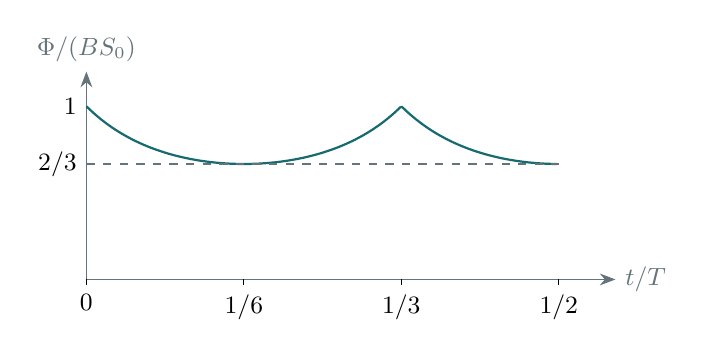
\begin{tikzpicture}[x=12cm,y=2.2cm,font=\small]
\draw[axis] (0,0)--(.56,0) node[right] {$t/T$};\draw[axis] (0,0)--(0,1.2) node[above] {$\Phi/(BS_0)$};
\draw[traj,domain=0:.5,samples=241,variable=\t] plot(\t,{(tan(mod(360*\t,120)/2)+tan(60-mod(360*\t,120)/2))/sqrt(3)});
\foreach \x/\lab in {0/0,.1666667/{1/6},.3333333/{1/3},.5/{1/2}}{\draw (\x,0)--(\x,-.03) node[below] {$\lab$};}
\draw[guide] (0,.6666667)--(.5,.6666667);\node[left] at (0,.6666667) {$2/3$};\node[left] at (0,1) {$1$};
\end{tikzpicture}
\figcaption{解图电3.1C　重叠面积决定磁通曲线。最低点有水平切线，完全重合处曲线左右斜率不同。}
\end{minipage}\end{center}

为求解图电3.1C上的瞬时磁通，取三角形内切圆半径$d=a/(2\sqrt3)$。
两个等边三角形的六条有效边都与此圆相切，其相邻外法线角交替为$\theta$与$2\pi/3-\theta$。
切线多边形面积为内切半径乘周长的一半，故在$0\le\theta\le2\pi/3$内
\[
S(\theta)=3d^2\left[\tan\frac\theta2+\tan\left(\frac\pi3-\frac\theta2\right)\right]
=\frac{a^2}{4}\left[\tan\frac\theta2+\tan\left(\frac\pi3-\frac\theta2\right)\right].
\]
两端为$S_0$，中点为$S_*$，对中点对称；在第一半段斜率为负，后一半段为正。
代$\theta=2\pi t/T$并按$T/3$延拓，就得到C图。曲线的下降段对应正电流，上升段对应反向电流。

解图电3.1B的 $D,E$ 分别将大三角形的两腰三等分。解图电3.1A中三个切角分居三个顶点，每个切角正对转动线框的一条边。对解图电3.1C，可将尖顶看作固定场区和转动线框恰好共用三条边的时刻。经过尖顶时面积连续，前后截去的区域互换，使瞬时电流由斜率的一侧值跳到另一侧值。对任意跨越该点的时间段，电量仍是连续磁通的端点差乘 $-1/R$。


\Needspace{13\baselineskip}

\pdfbookmark[2]{第 2 题 恒力收缩导线圆圈的闭合时间}{q2}

\section*{第 2 题\quad 恒力收缩导线圆圈的闭合时间}\label{q:2}

柔软导体回路$ABCDA$的总电阻恒为$R$，其中$AB$段的一部分绕成初始半径$r_0$的圆圈，圆圈处于垂直其平面的匀强磁场$B$中。$B$端固定，$C,D$端自由；沿$BA$方向对$A$端施加恒力$F$，使圆圈缓慢缩小并始终保持圆形。忽略导线惯性、自感、弹性储能和一切机械阻力，圆圈以外部分的磁通变化忽略不计。求半径缩至零的形式闭合时间$T$。

\begin{center}\begin{minipage}{.98\linewidth}\centering
\begin{tikzpicture}[scale=.85]

\draw[object] (-2,1.8) node[above left]{$B$（固定）}--(-.65,1.8)
.. controls(-.4,1.8) and(-.45,1.15)..(.17365,.98481)
arc(80:-260:1)
.. controls(.05,1.15) and(.35,1.8)..(.65,1.8)--(3.8,1.8) node[above]{$A$};
\draw[object] (3.8,1.8)--(3.8,-1.5) node[right]{$D$}--(-2,-1.5) node[left]{$C$}--(-2,1.8);
\draw[force] (4.1,1.8)--(5.4,1.8) node[right]{$F$};
\draw[axis] (0,0)--(-.707,-.707) node[midway,below]{$r_0$};\node at(.3,.2){$\odot B$};

\end{tikzpicture}\figcaption{图电3.2\quad 圆圈串在$AB$软线段中，交叉处不电接触；外部回路示意。}\end{minipage}\end{center}

\Needspace{6\baselineskip}\subsection*{解答}

解图电3.2A用$x$标记$A$端拉出的导线长度。圆圈的周长缩短多少，直线段就增加多少，故
\[
\dd x=-\dd(2\pi r)=-2\pi\dd r,\qquad \dot r<0.
\]
半径每减小一单位长度，直线段的增长量为 $2\pi$ 单位长度。

\begin{center}\begin{minipage}{.98\linewidth}\centering
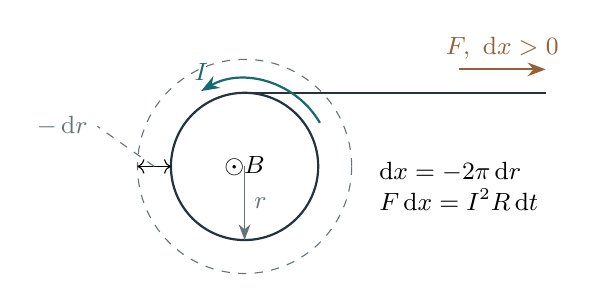
\begin{tikzpicture}[scale=.85]

\draw[guide] (0,0) circle(1.6);\draw[object] (0,0) circle(1.1);
\draw[axis] (0,0)--(0,-1.1) node[midway,right]{$r$};
\draw[<->] (-1.6,0)--(-1.1,0);\draw[guide] (-1.35,0)--(-2.2,.6) node[left]{$-\dd r$};
\draw[object] (0,1.1)--(4.5,1.1);\draw[force] (3.2,1.45)--(4.5,1.45) node[midway,above]{$F,\ \dd x>0$};
\draw[motion] (30:1.3) arc(30:120:1.3) node[above]{$I$};\node at(0,0){$\odot B$};
\node[align=left] at(3.2,-.3){$\dd x=-2\pi\dd r$\\$F\dd x=I^2R\dd t$};

\end{tikzpicture}\figcaption{解图电3.2A\quad 圆周缩短转为拉出长度；电流阻碍磁通减少。}\end{minipage}\end{center}

取圆圈内磁通的正方向与$B$一致。圆圈缩小时磁通减少，感应电流产生同向磁场。电动势、电流的大小分别为
\[
\mathcal E=-\frac{\dd(B\pi r^2)}{\dd t}
=-2\pi Br\dot r,\qquad
I=-\frac{2\pi Br}{R}\dot r.
\]
在规定的缓慢、无惯性模型中，机械功全部成为焦耳热：
\[
F\dd x=I^2R\dd t.
\]
代入几何约束与电流，在$r>0$的收缩阶段约去非零的$\dot r$，得到
\[
-2\pi F\dot r=\frac{4\pi^2B^2r^2}{R}\dot r^2,
\qquad
\dot r=-\frac{FR}{2\pi B^2r^2}.
\]
分离变量并使用$r(0)=r_0$：
\[
\int_{r_0}^{r}u^2\dd u=-\frac{FR}{2\pi B^2}\int_0^t\dd t,
\quad
r^3=r_0^3-\frac{3FR}{2\pi B^2}t.
\]
令$r=0$，得到
\[
\boxed{T=\frac{2\pi B^2r_0^3}{3FR}},\qquad
r(t)=r_0\left(1-\frac tT\right)^{1/3}.
\]
整个过程中，$A$ 端拉出长度$2\pi r_0$，因此总焦耳热为$Q=2\pi Fr_0$。由上式也得$I=F/(Br)$：临近$r=0$时电流和收缩速度发散。上式中的 $T$ 是准静态方程积分到 $r=0$ 的形式闭合时间。若只算到有限的小半径 $\varepsilon$，形式上继续收缩到零的时间为 $T(\varepsilon/r_0)^3$。

收缩末端的速度虽发散，电量与总热量的积分仍有限。将$\dd t=-2\pi B^2r^2\dd r/(FR)$代入，可得
\[
q_{\rm tr}=\int_0^T I\dd t
=-\frac{2\pi B}{R}\int_{r_0}^{0}r\dd r
=\frac{B\pi r_0^2}{R},
\]
\[
\int_0^T I^2R\dd t
=-2\pi F\int_{r_0}^{0}\dd r=2\pi Fr_0.
\]
电量等于磁通减少量除以 $R$，而热量等于恒力乘整个拉出长度。解图电3.2B把运动写成$r^3$的直线规律，便于看出后段所占的时间。

\begin{center}\begin{minipage}{.98\linewidth}\centering
\begin{tikzpicture}[scale=.85]

\draw[axis](0,0)--(5.2,0) node[right]{$t/T$};\draw[axis](0,0)--(0,2.8) node[above]{$r^3/r_0^3$};
\draw[traj](0,2.2)--(4.4,0);\node[left] at(0,2.2){$1$};\node[below right] at(4.4,0){$1$};
\draw[guide](3.85,0)--(3.85,.275)--(0,.275);\fill(3.85,.275) circle(1.5pt);
\node[below left] at(3.85,0){$7/8$};\node[left] at(0,.275){$1/8$};
\node[align=left] at(8,1.5){$r=r_0/2$时$t=7T/8$\\$r^3=r_0^3(1-t/T)$\\末段做功占总功一半};

\end{tikzpicture}\figcaption{解图电3.2B\quad 半径的立方随时间线性下降，半径的减小速率随时间增大。}\end{minipage}\end{center}

当 $r=r_0/2$ 时，$t/T=1-(1/2)^3=7/8$。此后在总历时的最后 $1/8$ 内拉出一半圆周长度，恒力在这段所做的功占总功的一半。

\begin{center}\begin{minipage}{.97\linewidth}\centering
\begin{tikzpicture}[x=1cm,y=1cm,font=\small]
\foreach \xx/\lab/\pow in {0/{I/I_0}/{1/3},4.5/{(-\dot r)/(-\dot r_0)}/{2/3}}{\begin{scope}[xshift=\xx cm]
\draw[axis] (0,0)--(3.2,0) node[right] {$t/T$};\draw[axis] (0,0)--(0,3) node[above] {$\lab$};
\draw[traj,domain=0:.88,samples=90,variable=\t] plot({3*\t},{.6*(1-\t)^(-\pow)});
\draw[guide] (3,0)--(3,2.85);\node[below] at (3,0) {$1$};\node[left] at (0,.6) {$1$};\end{scope}}
\end{tikzpicture}
\figcaption{解图电3.2C　用各自初值归一化的电流与收缩速率；均沿实际幂律绘制到$t/T=0.88$，虚线表示形式闭合时刻，曲线在此前已显示加速。}
\end{minipage}\end{center}

从圆圈截取张角为 $\dd\phi$ 的小弧。沿正向的感应电流在向外磁场中使小弧受到向外的磁力 $IBr\dd\phi$。软线张力近似等于端拉力 $F$ 时，小弧两端的切向张力合成向内的径向分量 $F\dd\phi$。无惯性的圆形收线模型给 $F=IBr$，说明同一个拉力在较小半径处需要较大的电流来平衡。

解图电3.2C由$r/r_0=(1-t/T)^{1/3}$直接给出
\[
\frac{I}{I_0}=(1-t/T)^{-1/3},\qquad
\frac{-\dot r}{-\dot r_0}=(1-t/T)^{-2/3},\qquad I_0=\frac{F}{Br_0}.
\]
临近 $T$，焦耳热功率按 $(T-t)^{-2/3}$ 增大。积分 $\int_{t_*}^T(T-t)^{-2/3}\dd t=3(T-t_*)^{1/3}$ 随余下时间 $T-t_*$ 减小而趋零。图B给出 $r_0/2$ 以下的收缩时间为 $T/8$。图C的电流迅速增大，热功率的积分在这段达到总热量的一半。这里的上升曲线适用于导线仍可视为圆形，且惯性与自感相对较小的阶段。


\Needspace{13\baselineskip}

\pdfbookmark[2]{第 3 题 铜环倾倒时的磁阻尼与能量}{q3}

\section*{第 3 题\quad 铜环倾倒时的磁阻尼与能量}\label{q:3}

细铜圆环的主半径$r_1=1.0\,\mathrm{cm}$，圆形导线截面半径$r_2=1.0\,\mathrm{mm}$。圆环竖放，底部有光滑固定栓限制滑动，使它可绕经过最低点的水平切线轴倾倒。竖直向上匀强磁场$B=1.0\,\mathrm T$。圆环由与竖直方向夹角$\theta_0=1.0\,\mathrm{rad}$的位置静止释放，最后到达水平位置。铜的电导率$\sigma=6.25\times10^7\,\mathrm{S/m}$，密度$\rho=8.93\times10^3\,\mathrm{kg/m^3}$，取$g=9.80\,\mathrm{m/s^2}$，忽略自感、空气阻力及接触耗散。
\begin{enumerate}
\item 通过估算和能量关系，判断重力势能如何分配；说明平均转速能否直接估计倒地瞬间的转动动能。
\item 在忽略角加速度项的准静态近似中，令磁阻力矩与重力矩相等，求从一般初始角$0<\theta_0<\pi/2$到水平位置的时间，并计算$\theta_0=1.0\,\mathrm{rad}$的结果。讨论近似的适用范围。
\end{enumerate}

\begin{center}\begin{minipage}{.98\linewidth}\centering
\begin{tikzpicture}[scale=.85]

\draw[object] (-1,0)--(3.2,0);\fill(0,0) circle(2pt) node[below]{$P$（栓轴）};
\draw[guide] (0,0)--(0,2.8);\draw[object,very thick] (0,0)--(2.6927,1.7290);
\fill(1.3464,.8645) circle(2pt) node[above]{$G$};\node at(.65,.18){$r_1$};
\draw (0,.85) arc(90:32.7042:.85);\node at(.48,1.02){$\theta_0$};
\foreach \x in {4,4.7,5.4}{\draw[motion] (\x,.2)--(\x,2.8);}\node at(4.7,3.2){$B$};
\node at(-.9,2.3){侧视};\node at(7.5,2.2){导线截面};\draw[object] (7.5,1.1) circle(.4);
\draw[axis] (7.5,1.1)--(7.9,1.1) node[midway,above]{$r_2$};

\end{tikzpicture}\figcaption{图电3.3\quad 初始环面倾角为$1.0\,\mathrm{rad}$；重心$G$距栓轴为$r_1$。}\end{minipage}\end{center}

\Needspace{6\baselineskip}\subsection*{解答}

解图电3.3A取圆环平面相对竖直方向的倾角$\theta$，角速度$\omega=\dot\theta$。主半径远大于导线截面半径，先用细环近似计算质量、电阻、转动惯量：
\[
m=2\pi^2\rho r_1r_2^2,\qquad
R_e=\frac{2\pi r_1}{\sigma\pi r_2^2}=\frac{2r_1}{\sigma r_2^2},\qquad
J=\frac12mr_1^2+mr_1^2=\frac32mr_1^2.
\]
导线的长度为 $2\pi r_1$，横截面积为 $\pi r_2^2$。最后一式先取过圆心且与栓轴平行的直径轴，再以 $r_1$ 为轴间距使用平行轴定理。

\begin{center}\begin{minipage}{.98\linewidth}\centering
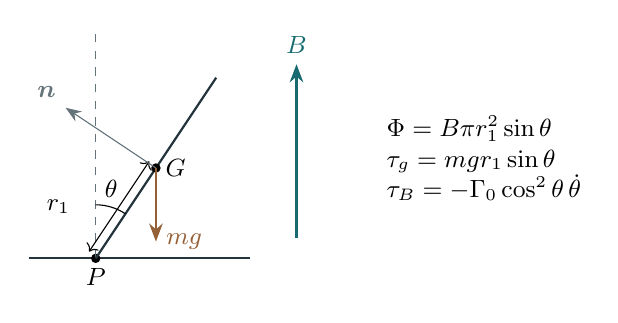
\begin{tikzpicture}[scale=.85]

\draw[object] (-1,0)--(2.3,0);\fill (0,0) circle(2pt) node[below]{$P$};
\draw[guide] (0,0)--(0,3.4);\draw[object] (0,0)--(1.8,2.7);
\fill (.9,1.35) circle(2pt) node[right]{$G$};\draw[force] (.9,1.35)--(.9,.25) node[right]{$mg$};
\draw[<->] (-.1,.1)--(.8,1.45) node[midway,left,xshift=-5mm]{$r_1$};
\draw (0,.8) arc(90:56.3:.8) node[midway,above]{$\theta$};
\draw[motion] (3,.3)--(3,2.9) node[above]{$B$};
\draw[axis] (.9,1.35)--(-.45,2.25) node[above left]{$\vect n$};
\node[align=left] at(5.8,1.5){$\Phi=B\pi r_1^2\sin\theta$\\$\tau_g=mg r_1\sin\theta$\\$\tau_B=-\Gamma_0\cos^2\theta\,\dot\theta$};

\end{tikzpicture}\figcaption{解图电3.3A\quad 法线投影决定磁通，重心横移决定重力矩。}\end{minipage}\end{center}

环面磁通量为$\Phi=B\pi r_1^2\sin\theta$，因此感应电流大小为
\[
I=\frac{B\pi r_1^2}{R_e}\cos\theta\,\dot\theta.
\]
磁矩与$B$的夹角使磁阻力矩为
\[
M_B=I\pi r_1^2B\cos\theta
=\Gamma_0\cos^2\theta\,\dot\theta,
\qquad \Gamma_0=\frac{B^2\pi^2r_1^4}{R_e}.
\]
它阻碍倾倒，重力矩为$M_g=mg r_1\sin\theta$。完整运动与能量方程是
\[
J\ddot\theta=mg r_1\sin\theta-\Gamma_0\cos^2\theta\,\dot\theta,
\qquad \theta(0)=\theta_0,\quad\dot\theta(0)=0,
\]
\[
\frac{\dd}{\dd t}\left(\frac12J\dot\theta^2+mg r_1\cos\theta\right)
=-\Gamma_0\cos^2\theta\,\dot\theta^2=-I^2R_e.
\]
故到水平位置时，严格的能量关系为
\[
\boxed{mg r_1\cos\theta_0=Q+\frac12J\omega_f^2}.
\]
判断耗散强弱可比较重力运动时间$t_g=\sqrt{J/(mg r_1)}$与阻尼参数$K=\Gamma_0/(mg r_1)$：
\[
t_g\simeq0.0391\,\mathrm s,\qquad
K=\frac{\sigma B^2r_1}{4\rho g}\simeq1.785\,\mathrm s.
\]
$K/t_g\simeq45.6$。在 $\cos^2\theta$ 仍较大的角区，磁阻尼使运动缓慢。接近水平位置时，解图电3.3B的 $\cos^2\theta$ 迅速趋零，重力矩却接近 $mg r_1$，于是圆环最后一段加速。末动能由此时的瞬时角速度 $\omega_f$ 给出。

\begin{center}\begin{minipage}{.98\linewidth}\centering
\begin{tikzpicture}[scale=.85]

\draw[axis] (0,0)--(5.5,0) node[right]{$\theta$};\draw[axis] (0,0)--(0,2.7) node[above]{$\Gamma/\Gamma_0$};
\draw[traj,domain=0:90,samples=70] plot ({\x/20},{2*cos(\x)^2});
\node[left] at(0,2){$1$};\node[below] at(4.5,0){$\pi/2$};
\node[align=left] at(7.6,1.3){$\Gamma=\Gamma_0\cos^2\theta$\\临近水平时阻尼衰减\\末段重力矩仍接近最大值};

\end{tikzpicture}\figcaption{解图电3.3B\quad 阻尼系数随倾角下降，在水平位置降为零。}\end{minipage}\end{center}

例如按上述完整初值方程作数值积分，题给$\theta_0=1.0\,\mathrm{rad}$时，倾倒时间约$0.141\,\mathrm s$，$\omega_f\simeq16.16\,\mathrm{rad/s}$，从而
\[
\frac{\tfrac12J\omega_f^2}{mg r_1\cos\theta_0}\simeq0.370,
\qquad \frac{Q}{mg r_1\cos\theta_0}\simeq0.630.
\]
在这个初始角下，重力释放的能量多数成为焦耳热，其余成为末态动能。初始角改为 $0.10\,\mathrm{rad}$ 时，用到达末态的瞬时转速计算，末态动能占比仍约为 $0.201$。

\begin{center}\begin{minipage}{.97\linewidth}\centering
\begin{tikzpicture}[x=5cm,y=3cm,font=\small]
\draw[axis] (0,0)--(1.12,0) node[right] {$u$};\draw[axis] (0,0)--(0,.85) node[above] {能量$/\Delta U_g$};
\draw[traj] plot coordinates {(0.000000,0.000000) (0.003047,0.001477) (0.009435,0.002807) (0.017126,0.003478) (0.025389,0.003831) (0.033965,0.004062) (0.042761,0.004251) (0.051748,0.004431) (0.060922,0.004615) (0.070284,0.004808) (0.079841,0.005013) (0.089603,0.005232) (0.099580,0.005468) (0.109782,0.005722) (0.120221,0.005996) (0.130911,0.006292) (0.141867,0.006613) (0.153103,0.006962) (0.164637,0.007342) (0.176487,0.007758) (0.188675,0.008215) (0.201223,0.008717) (0.214156,0.009271) (0.227503,0.009886) (0.241294,0.010570) (0.255564,0.011334) (0.270353,0.012193) (0.285705,0.013162) (0.301671,0.014261) (0.318307,0.015517) (0.335679,0.016958) (0.353863,0.018626) (0.372945,0.020568) (0.393027,0.022850) (0.414229,0.025554) (0.436691,0.028787) (0.460580,0.032694) (0.486095,0.037468) (0.513478,0.043371) (0.543021,0.050763) (0.575079,0.060145) (0.610091,0.072217) (0.648595,0.087968) (0.691254,0.108784) (0.738876,0.136579) (0.792432,0.173891) (0.853038,0.223767) (0.921881,0.289027) (1.000000,0.370086)};
\draw[thick,warm] plot coordinates {(0.000000,0.000000) (0.003047,0.001233) (0.009435,0.005595) (0.017126,0.011794) (0.025389,0.018844) (0.033965,0.026318) (0.042761,0.034056) (0.051748,0.042001) (0.060922,0.050136) (0.070284,0.058460) (0.079841,0.066977) (0.089603,0.075694) (0.099580,0.084622) (0.109782,0.093769) (0.120221,0.103146) (0.130911,0.112766) (0.141867,0.122641) (0.153103,0.132784) (0.164637,0.143211) (0.176487,0.153937) (0.188675,0.164980) (0.201223,0.176359) (0.214156,0.188094) (0.227503,0.200207) (0.241294,0.212723) (0.255564,0.225669) (0.270353,0.239072) (0.285705,0.252963) (0.301671,0.267378) (0.318307,0.282352) (0.335679,0.297926) (0.353863,0.314140) (0.372945,0.331040) (0.393027,0.348672) (0.414229,0.367081) (0.436691,0.386313) (0.460580,0.406403) (0.486095,0.427375) (0.513478,0.449229) (0.543021,0.471922) (0.575079,0.495341) (0.610091,0.519260) (0.648595,0.543278) (0.691254,0.566731) (0.738876,0.588580) (0.792432,0.607339) (0.853038,0.621159) (0.921881,0.628473) (1.000000,0.629914)};
\node[right,warm] at (1.08,.64) {$Q/\Delta U_g\simeq0.630$};
\node[right,accent] at (1.08,.37) {$K_{\rm rot}/\Delta U_g\simeq0.370$};
\node[below] at (1,0) {$1$};\node[below] at (.5,-.23) {$u=(\theta-\theta_0)/(\pi/2-\theta_0)$};
\end{tikzpicture}
\figcaption{解图电3.3C　题给$\theta_0=1.0$的完整初值方程数值解。横轴按已经倾倒的角度归一化；热量曲线对瞬时耗散率积分得到，动能曲线取每个倾角处的瞬时角速度。}
\end{minipage}\end{center}

\textbf{准静态时间。}第二问明确略去$J\ddot\theta$，于是
\[
\Gamma_0\cos^2\theta\,\dot\theta=mg r_1\sin\theta,
\qquad \dd t=K\frac{\cos^2\theta}{\sin\theta}\dd\theta.
\]
将被积函数写成$\csc\theta-\sin\theta$，逐项积分：
\[
T_{\rm qs}=K\int_{\theta_0}^{\pi/2}\frac{\cos^2\theta}{\sin\theta}\dd\theta
=K\left[\ln\tan\frac\theta2+\cos\theta\right]_{\theta_0}^{\pi/2},
\]
\[
\boxed{T_{\rm qs}=\frac{\sigma B^2r_1}{4\rho g}
\left[-\ln\tan\frac{\theta_0}{2}-\cos\theta_0\right]}.
\]
取$\theta_0=1.0\,\mathrm{rad}$得$T_{\rm qs}\simeq0.115\,\mathrm s$；取$0.10\,\mathrm{rad}$则得$3.57\,\mathrm s$。两个初始角到水平的余下转角不同，且阻尼最大的角区接近竖直。准静态式适用于角加速度相对较小的中段。释放后的短暂调整阶段与水平位置附近均需保留惯性项，最后的角速度由初值方程给出。

准静态近似的误差还可在角度上作估计。令$\omega_{\rm qs}=\sin\theta/(K\cos^2\theta)$，沿这一近似轨迹求导，得到
\[
\ddot\theta_{\rm qs}=\omega_{\rm qs}\frac{\dd\omega_{\rm qs}}{\dd\theta}
=\frac{\sin\theta(1+\sin^2\theta)}{K^2\cos^5\theta},
\]
\[
\epsilon_{\rm in}=\frac{J|\ddot\theta_{\rm qs}|}{mg r_1\sin\theta}
=\left(\frac{t_g}{K}\right)^2\frac{1+\sin^2\theta}{\cos^5\theta}.
\]
当 $\epsilon_{\rm in}\ll1$ 时，准静态轨迹上所需的惯性力矩远小于重力矩，磁阻力矩和重力矩近似平衡。对本题参数，在$\theta=1.0$处该比值约为$0.018$，但临近水平时按$\cos^{-5}\theta$增长。取终端$1+\sin^2\theta\simeq2$估计，$\epsilon_{\rm in}\sim1$约发生在$\pi/2-\theta\sim[2(t_g/K)^2]^{1/5}\simeq0.25\,\mathrm{rad}$。进入这一角区后，角加速度与重力矩同阶贡献。释放瞬间又有$\dot\theta=0$，也需经历建立阻尼速度的短暂调整。这个角度判据与解图电3.3B的阻尼趋零相对应。


\textbf{平均电流与总热量。} 解图电3.3C取$\Delta U_g=mgr_1\cos\theta_0$，从释放点逐步积分瞬时热功率。
平均电流满足$\overline I\,T=|\Delta\Phi|/R_e$，但焦耳热为$R_eT\overline{I^2}$；
用 $\overline{I^2}\ge\overline I^2$ 可得
\[
Q\ge\frac{B^2\pi^2r_1^4(1-\sin\theta_0)^2}{R_eT}.
\]
热量比下界多出的部分为 $R_e\int_0^T(I-\overline I)^2\dd t$。转动平均角速度 $(\pi/2-\theta_0)/T$ 给总转角与历时的比。重力在最后的弱阻尼区仍做正功，角速度持续上升，解图电3.3C中的末动能取最后时刻的 $\omega_f$。

按图A的力矩方向积分，采用状态$\theta,\omega,Q$，并单独加入$\dot Q=\Gamma_0\cos^2\theta\,\omega^2$，
以到达 $\theta=\pi/2$ 为停止事件，从最后的状态读取转速和热量。题给参数得到 $T\simeq0.14066\,\mathrm s$、$\omega_f\simeq16.1641\,\mathrm{rad/s}$。解图电3.3C显示，在最后几个转角内热量曲线接近水平，重力势能损失主要进入转动动能。第二问将中段的准静态积分延伸至水平，得到形式时间 $T_{\rm qs}\simeq0.115\,\mathrm s$。

第二问积分还可写成
\[
T_{\rm qs}=K\left[-\cos\theta_0+\frac12\ln\frac{1+\cos\theta_0}{1-\cos\theta_0}\right],
\]
因$-\ln\tan(\theta_0/2)=\tfrac12\ln[(1+\cos\theta_0)/(1-\cos\theta_0)]$，与前式严格相同。
这个形式直接用初始高度的无量纲比值 $\cos\theta_0$ 来算。当 $\theta_0$ 减小时，分母 $1-\cos\theta_0$ 与 $\theta_0^2/2$ 同阶，因而用时会按初始角的对数增长。


\Needspace{13\baselineskip}

\pdfbookmark[2]{第 4 题 翻转线圈测地磁场的分支判断}{q4}

\section*{第 4 题\quad 翻转线圈测地磁场的分支判断}\label{q:4}

水平桌面上有矩形线圈$abcd$，$ab=\ell_1$指向北方，$bc=\ell_2$沿东西方向，总电阻为$R$，面积$S=\ell_1\ell_2$。先绕南北方向的中心轴翻转$180^\circ$，使$ab$与$cd$交换位置，测得通过导线的净电量绝对值为$Q_1$。再固定南侧的$ad$边，将北侧边抬起$90^\circ$使线圈竖直；线圈从水平状态的向上法线转向南方，测得这次净电量绝对值为$Q_2$。地磁场的水平分量向北，竖直分量可向上或向下。忽略自感。
求地磁场大小的可能值及各分支的条件；说明还需记录什么信息才能消除歧义。净电量指$\int I\dd t$，不等同于累计电量$\int|I|\dd t$。

\begin{center}\begin{minipage}{.98\linewidth}\centering
\begin{tikzpicture}[scale=.85]

\draw[object] (0,0) node[below left]{$a$}--(0,2.5) node[above left]{$b$}--(4,2.5) node[above right]{$c$}--(4,0) node[below right]{$d$}--cycle;
\draw[axis] (5,0)--(5,2) node[above]{北};\draw[axis] (5,0)--(6.5,0) node[right]{东};
\draw[<->] (-.5,0)--(-.5,2.5) node[midway,left]{$\ell_1$};\draw[<->] (0,-.6)--(4,-.6) node[midway,below]{$\ell_2$};
\draw[guide] (2,-.2)--(2,2.9);\node at(2,4){先绕南北轴翻转$180^\circ$};
\draw[motion] (.5,2.8)--(.5,3.4);\node at(5.7,3.4){再抬北边};

\end{tikzpicture}\figcaption{图电3.4\quad 俯视矩形及两次操作，第二步固定南边$ad$。}\end{minipage}\end{center}

\Needspace{6\baselineskip}\subsection*{解答}

解图电3.4A取向北为$+y$、向上为$+z$，写地磁场为
\[
\vect B=B_H\vect e_y+B_z\vect e_z,\qquad B_H\ge0.
\]
第一步翻转使有向面积法线反向，磁通变化的绝对值为$2S|B_z|$。由$R\int I\dd t=-\Delta\Phi$，得
\[
b\equiv|B_z|=\frac{RQ_1}{2S}.
\]

\begin{center}\begin{minipage}{.98\linewidth}\centering
\begin{tikzpicture}[scale=.85]

\draw[axis] (0,0)--(3,0) node[right]{北$\ (+y)$};\draw[axis] (0,0)--(0,2.8) node[above]{上$\ (+z)$};
\draw[motion] (0,0)--(0,2) node[left]{$\vect n_i$};\draw[motion] (0,0)--(-2,0) node[left]{$\vect n_f$};
\draw[force] (0,0)--(2,-1.4) node[right]{$\vect B=B_H\vect e_y-b\vect e_z$};
\draw[guide] (2,0)--(2,-1.4)--(0,-1.4);\node[below] at(1,0){$B_H$};\node[left] at(0,-1.1){$b$};
\node[align=left] at(6,1.4){第二步初法线：向上\\末法线：向南\\$\Delta\Phi=S(b-B_H)$};

\end{tikzpicture}\figcaption{解图电3.4A\quad 示出竖直场向下的分支；第二步的法线由上转向南。}\end{minipage}\end{center}

第二步开始时法线为$+\vect e_z$，最后为$-\vect e_y$，所以
\[
\Phi_i=SB_z,\quad\Phi_f=-SB_H,\quad
c\equiv\frac{RQ_2}{S}=|B_H+B_z|.
\]
两次读数分别确定 $|B_z|$ 和 $|B_H+B_z|$。下面令 $B_z$ 向上或向下，再由第二个绝对值方程求 $B_H$。

\textbf{竖直分量向下。}此时$B_z=-b$，有$|B_H-b|=c$，因此
\[
B_H=b+c\quad\hbox{或}\quad B_H=b-c\ (b\ge c).
\]
两种磁场大小为
\[
\boxed{B=\sqrt{b^2+(b+c)^2}},\qquad
\boxed{B=\sqrt{b^2+(b-c)^2}\quad(b\ge c)}.
\]
第一式对应水平分量不小于向下分量；第二式对应水平分量不大于向下分量。写成读数为
\[
B=\frac{R}{\sqrt2S}\sqrt{Q_1^2\pm2Q_1Q_2+2Q_2^2},
\]
其中负号要求$Q_1\ge2Q_2$。

\textbf{竖直分量向上。}此时$B_z=b$，有$B_H+b=c$，故
\[
\boxed{B_H=c-b,\quad
B=\sqrt{b^2+(c-b)^2}\quad(c\ge b)}.
\]
它的存在条件是$2Q_2\ge Q_1$。在$b=c$处，向下场的第二支与向上场的水平分量均为零；两种竖直方向给同一场强大小 $b$。

若$Q_1=0$，竖直分量为零，直接由第二次读数得$B=B_H=RQ_2/S$。一般情况下，由独立测量知道地磁场向上或向下，可以确定 $B_z$ 的符号；对向下场，还需要第二次净电量的有向符号，才能判断$B_H-b$的符号。此时 $q_2>0$ 对应 $B_H>b$，$q_2<0$ 对应 $B_H<b$。

\begin{center}\begin{minipage}{.98\linewidth}\centering
\begin{tikzpicture}[scale=.85]

\draw[axis] (0,0)--(3,0) node[right]{北};\draw[axis] (0,0)--(0,2.8) node[above]{上};
\draw[traj] (0,2) arc(90:180:2);\draw[motion] (0,0)--(-1.4,1.4) node[above left]{$\vect n(\alpha)$};
\draw (0,.7) arc(90:135:.7) node[midway,above]{$\alpha$};
\node[align=left] at(5.9,1.4){$\Phi=-S(b\cos\alpha+B_H\sin\alpha)$\\$|\Phi|$可先增后减\\净电量会发生抵消};

\end{tikzpicture}\figcaption{解图电3.4B\quad 向下场中的磁通先降后升，两个区间的电流方向相反。}\end{minipage}\end{center}

解图电3.4B还说明第二次操作的测量含义。若竖直场向下，抬起角为$\alpha$时
\[
\Phi(\alpha)=-S(b\cos\alpha+B_H\sin\alpha).
\]
磁通可能先减小后增大，电流随之反向。冲击式净电量读数仍由两个端点相减确定，累计电量则从磁通极小点处分段，各段分别取绝对值再相加。

若实验同时记录电流方向，就可以把两个绝对值还原为两个线性关系。规定导线正向始终跟随$a\to b\to c\to d\to a$的材料标号；第一步前这个方向的法线向下，翻转后向上。记相应的有向净电量为$q_1,q_2$，则
\[
Rq_1=-2SB_z,\qquad Rq_2=S(B_H+B_z),
\]
\[
B_z=-\frac{Rq_1}{2S},\qquad
B_H=\frac R S\left(q_2+\frac{q_1}{2}\right).
\]
两条有向方程给出唯一的 $B_z,B_H$，其中向北为 $B_H\ge0$。由平方和开方得到 $B=\sqrt{B_H^2+B_z^2}$。在解图电3.4A中，纯水平场与第一次翻转的水平积分面平行，所以 $q_1=0$。纯竖直场在第二次翻转的终态与线圈平面平行，故第二次的净电量大小为第一次的一半。

\begin{center}\begin{minipage}{.97\linewidth}\centering
\begin{tikzpicture}[x=2cm,y=1cm,font=\small]
\draw[axis] (0,0)--(2.25,0) node[right] {$c/b$};\draw[axis] (0,0)--(0,3.5) node[above] {$B_H/b$};
\draw[traj] (0,1)--(2,3);\draw[traj] (0,1)--(1,0);
\draw[thick,warm,dashed] (1,0)--(2,1);
\draw[guide] (1,0)--(1,3.2);\node[below] at (1,0) {$1$};\node[left] at (0,1) {$1$};
\node[right,accent] at (2.15,2.7) {$B_z=-b$，$B_H=b+c$};
\node[right,accent] at (2.15,2.1) {$B_z=-b$，$B_H=b-c$};
\node[right,warm] at (2.15,1.4) {$B_z=+b$，$B_H=c-b$};
\node[right] at (2.15,.6) {$b>0$；负的水平分量舍去};
\end{tikzpicture}
\figcaption{解图电3.4C　两个绝对值读数对应的全部非负水平分量。实线为向下场两支，虚线为向上场支；交于横轴的两种竖直场方向仍不同。}
\end{minipage}\end{center}

解图电3.4C把存在条件放在读数坐标中：$c<b$时仅有向下场，但仍有两个不同的水平分量；
$c>b$时向下场大根与向上场根同时存在；$c=b$时另有水平分量为零的极限。
若只问B的大小，两个小根的平方形式可以写成同一个根式，但对应的竖直方向仍须分别说明。
当$c=0$且$b>0$时，向下场两式重合为$B_H=b$，两支给同一场强大小。若 $b=c=0$，两个分量同时为零。

翻转携带材料标号，也携带回路正向。题图俯视$a\to b\to c\to d$的初法线向下，第一次翻转后向上；
随后固定南边抬起北边，法线从向上转至向南，正是图A、B所用的第二步法线。
依同一材料绕向，在两步中连续跟踪法线并记录两个有向电量。若整组实验改用反向绕行，两个 $q_i$ 同时换号，法线也一同反向，所得场分量保持。

对解图电3.4B中的向下场，取 $b,B_H>0$，
$\Phi'(\alpha)=S(b\sin\alpha-B_H\cos\alpha)$在$\tan\alpha=B_H/b$改变符号。
因此一次看似简单的竖起操作也会先后出现相反电流。把完整电流波形带符号积分，极小点前后的两段电量部分相消，余量仍为两个端点磁通之差乘 $-1/R$。


\Needspace{13\baselineskip}

\pdfbookmark[2]{第 5 题 双格线框移出磁场的外力功}{q5}

\section*{第 5 题\quad 双格线框移出磁场的外力功}\label{q:5}

“日”字形闭合导线框$abcdef$如图，$a,f,e$在上边，$b,c,d$在下边，三条竖边$ab,fc,ed$等长，$ab=bc=cd=de=ef=fa=\ell=0.10\,\mathrm m$。$ab,fc,de$的电阻均为$R=3.0\,\Omega$，$cd,fe$均为$r=1.5\,\Omega$，$bc,af$电阻忽略。线框起初全部位于$B=1.0\,\mathrm T$的匀强磁场内，磁场垂直框面向里，右侧直边界与$de$平行。以$v=24\,\mathrm{m/s}$向右匀速拉出整个线框，忽略自感。求拉力做的总功。

\begin{center}\begin{minipage}{.98\linewidth}\centering
\begin{tikzpicture}[scale=.85]

\fill[accent!7] (-.7,-.5) rectangle (4.1,3.3);\draw[guide] (4.1,-.5)--(4.1,3.3) node[above]{场区边界};
\draw[object] (0,0) node[below]{$b$}--(0,2.4) node[above]{$a$}--(2.4,2.4) node[above]{$f$}--(4.8,2.4) node[above]{$e$}--(4.8,0) node[below]{$d$}--(2.4,0) node[below]{$c$}--cycle;
\draw[object] (2.4,0)--(2.4,2.4);\node[left] at(0,1.2){$R$};\node[right] at(2.4,1.2){$R$};\node[right] at(4.8,1.2){$R$};
\node[above] at(3.6,2.4){$r$};\node[below] at(3.6,0){$r$};\node at(1,1.2){$\otimes B$};
\draw[motion] (5.5,1.2)--(6.7,1.2) node[right]{$v$};

\end{tikzpicture}\figcaption{图电3.5\quad 两格均为边长$\ell$的正方形；图示右边已离开场区。}\end{minipage}\end{center}

\Needspace{6\baselineskip}\subsection*{解答}

题图电3.5中，三条竖边同时在磁场内时，它们的动生电动势相同，各闭合回路的净电动势为零，没有持续电流。开始需要做功的阶段，是$ed$刚移出磁场后。由于$af,bc$为理想导线，$a,f$等势、$b,c$等势；右侧折线路径$f\to e\to d\to c$的电阻为
\[
R_3=2r+R=6.0\,\Omega.
\]
每条仍在磁场内的竖边，其向上动生电动势大小均为
\[
\mathcal E=B\ell v=2.4\,\mathrm V.
\]

\begin{center}\begin{minipage}{.98\linewidth}\centering
\begin{tikzpicture}[scale=.82]

\draw[object] (0,0)--(5,0) (0,3)--(5,3);
\foreach \x/\lab in {0/{ab},2.5/{fc},5/{fedc}}{
\draw[object] (\x,0)--(\x,3);\node[above] at(\x,3){$\lab$};}
\node[fill=white] at(0,1.1){$R$};\node[fill=white] at(2.5,1.1){$R$};\node[fill=white] at(5,1.7){$R_3=2r+R$};
\draw[motion] (.2,.5)--(.2,2.3) node[midway,right]{$\mathcal E$};
\draw[force] (-.5,.6)--(-.5,1.5) node[left]{$I_{ab}$};
\draw[force] (5.7,1.2)--(5.7,.3) node[right]{$I_3$};
\node at(7.5,2.7){$U_1$：上减下};
\draw[motion] (2.7,.5)--(2.7,2.3) node[midway,right]{$\mathcal E$};\node at(2.5,-.7){$ab,fc$仍切割磁场};
\end{tikzpicture}\figcaption{解图电3.5A\quad 仍在磁场内的运动竖边才带动生电动势。}\end{minipage}\end{center}

\textbf{阶段一：只有$ed$在场外。}解图电3.5A有两条含电动势$\mathcal E$、电阻$R$的并联支路，另一条是无电动势的$R_3$支路。设上母线相对下母线的电势差为$U_1$，两电源支路电流向上，右支路电流向下，则
\[
I_{ab}=I_{fc}=\frac{\mathcal E-U_1}{R},\qquad
I_3=\frac{U_1}{R_3},\qquad 2\frac{\mathcal E-U_1}{R}=\frac{U_1}{R_3}.
\]
由此
\[
U_1=\frac{2R_3\mathcal E}{R+2R_3}=1.92\,\mathrm V,
\quad I_{ab}=I_{fc}=0.16\,\mathrm A.
\]
两竖边电流均向上，在向里磁场中受向左磁力。$ed$虽有电流，已经处于场外，因此该边所受磁力为零。拉力为
\[
F_1=B\ell(I_{ab}+I_{fc})=0.032\,\mathrm N.
\]
从$ed$出场到$fc$出场，位移为一格宽$\ell$，所以$W_1=F_1\ell=3.2\times10^{-3}\,\mathrm J$。

\begin{center}\begin{minipage}{.98\linewidth}\centering
\begin{tikzpicture}[scale=.82]

\draw[object] (0,0)--(5,0) (0,3)--(5,3);
\foreach \x/\lab in {0/{ab},2.5/{fc},5/{fedc}}{
\draw[object] (\x,0)--(\x,3);\node[above] at(\x,3){$\lab$};}
\node[fill=white] at(0,1.1){$R$};\node[fill=white] at(2.5,1.1){$R$};\node[fill=white] at(5,1.7){$R_3=2r+R$};
\draw[motion] (.2,.5)--(.2,2.3) node[midway,right]{$\mathcal E$};
\draw[force] (-.5,.6)--(-.5,1.5) node[left]{$I_{ab}$};
\draw[force] (5.7,1.2)--(5.7,.3) node[right]{$I_3$};
\node at(7.5,2.7){$U_2$：上减下};
\draw[force] (2.9,2.3)--(2.9,.7) node[midway,right]{$I_{fc}$};\node at(2.5,-.7){仅$ab$仍切割磁场};
\end{tikzpicture}\figcaption{解图电3.5B\quad 仍在磁场内的运动竖边才带动生电动势。}\end{minipage}\end{center}

\textbf{阶段二：$ed,fc$都在场外。}解图电3.5B只剩$ab$支路含电动势；$fc$支路仍有电阻$R$，右侧路径仍为$R_3$。此时
\[
\frac{\mathcal E-U_2}{R}=\frac{U_2}{R}+\frac{U_2}{R_3},
\quad U_2=0.96\,\mathrm V,
\quad I_{ab}=\frac{2.4-0.96}{3}=0.48\,\mathrm A.
\]
只有$ab$还在磁场内，故$F_2=B\ell I_{ab}=0.048\,\mathrm N$。这一阶段同样移动$\ell$，得$W_2=4.8\times10^{-3}\,\mathrm J$。总功为
\[
\boxed{W=W_1+W_2=8.0\times10^{-3}\,\mathrm J}.
\]
匀速时外力功率等于 $\sum I_j\mathcal E_j=\sum I_j^2R_j$，其中按同一方向取支路的电流和电动势。计算总热功率时，解图电3.5A、B的三条电阻支路都各贡献一项，两根理想母线的贡献为零：
\[
P_1=2(0.16)^2\times3+(0.32)^2\times6=0.768\,\mathrm W,
\]
\[
P_2=(0.48)^2\times3+(0.32)^2\times3+(0.16)^2\times6
=1.152\,\mathrm W.
\]
因此$P_1/v=0.032\,\mathrm N$、$P_2/v=0.048\,\mathrm N$，与两次安培力求和一致。每阶段历时$\Delta t=\ell/v=1/240\,\mathrm s$，总热量$(P_1+P_2)\Delta t=8.0\times10^{-3}\,\mathrm J$。第二阶段，场外的 $fc$ 已改为上节点流向下节点。它和右侧支路一起分担 $ab$ 提供的功率。

\begin{center}\begin{minipage}{.97\linewidth}\centering
\begin{tikzpicture}[x=2.5cm,y=3cm,font=\small]
\fill[accent!12] (0,0) rectangle(1,.4);\fill[warm!12] (1,0) rectangle(2,.6);
\draw[axis] (-.25,0)--(2.45,0) node[right] {$x/\ell$};\draw[axis] (0,0)--(0,.85) node[above] {$F/(B\ell\mathcal E/R)$};
\draw[traj] (-.2,0)--(0,0);\draw[traj] (0,.4)--(1,.4);
\draw[thick,warm] (1,.6)--(2,.6);\draw[traj] (2,0)--(2.3,0);
\foreach \x/\lab in {0/0,1/1,2/2}{\node[below] at(\x,0){$\lab$};\draw[guide] (\x,0)--(\x,.7);}
\node[left] at (0,.4) {$0.4$};\node[left] at (0,.6) {$0.6$};
\node at (.5,.18) {阶段一};\node at (1.5,.3) {阶段二};
\end{tikzpicture}
\figcaption{解图电3.5C　以$ed$刚出场为$x=0$，两段实际拉力平台及做功面积。三条竖边均在场内或均在场外时拉力为零；两个平台的端点由场区的直线分界确定。}
\end{minipage}\end{center}

解图电3.5C的两个横向区间均长一格，纵向高度却不同。
图A中$a,f$连成上节点、$b,c$连成下节点；两条相同的电源支路各向上送出0.16A，右侧整条折线路径接收0.32A。
图B中$ab$仍向上送出0.48A，$fc$改为向下0.32A，右支路仍向下0.16A。
图 A 的上节点流入为 $0.16+0.16$ A，与右支路流出相等。图 B 的上节点流入为 $0.48$ A，与 $0.32+0.16$ A 的总流出相等。

场内水平导线的安培力 $I\dd\boldsymbol l\times\boldsymbol B$ 指向框面内与运动垂直的方向，其沿位移方向的分量为零。场中竖直边的磁力平行于运动方向，计入水平阻力。场外的 $ed$ 和随后移出磁场的 $fc$ 仍在闭合网络中；它们所处位置 $B=0$，磁力为零。
因此第二阶段受水平磁力的边由两条减为一条，阻力仍可增加，原因是该边电流增为原来的三倍。

以 $ed$ 刚出场为位移零点，$x=\ell$ 时 $fc$ 的动生电动势由 $\mathcal E$ 变为零，$x=2\ell$ 时 $ab$ 也出场。由于题设忽略自感，电流即取各阶段的节点解，故解图电3.5C的做功面积为两个长方形的面积。


\Needspace{13\baselineskip}

\pdfbookmark[2]{第 6 题 双导体棒的速度趋同与间距上限}{q6}

\section*{第 6 题\quad 双导体棒的速度趋同与间距上限}\label{q:6}

水平面内有两条足够长的光滑平行理想导轨，间距为$\ell$，处于垂直纸面向里的匀强磁场$B$中。两根相同导体棒跨接在导轨上，每根长$\ell$、质量$m$、电阻$R$，组成闭合回路。忽略自感，初始左棒静止、右棒以$v_0$向右运动。求右棒速度$v_1(t)$和两棒间距增加量$x(t)$及其上限。

\begin{center}\begin{minipage}{.98\linewidth}\centering
\begin{tikzpicture}[scale=.85]

\draw[object] (-1,0)--(6,0) (-1,2.4)--(6,2.4);
\draw[object,very thick] (0,0)--(0,2.4) (4,0)--(4,2.4);
\node[left] at(0,1.2){$m,R$};\node[right] at(4,1.2){$m,R$};\node at(2,1.2){$\otimes B$};
\draw[motion] (4,2.8)--(5.4,2.8) node[right]{$v_0$};\node at(0,3){初始静止};
\draw[<->] (-1.4,0)--(-1.4,2.4) node[midway,left]{$\ell$};

\end{tikzpicture}\figcaption{图电3.6\quad 两棒与理想导轨形成总电阻$2R$的回路。}\end{minipage}\end{center}

\Needspace{6\baselineskip}\subsection*{解答}

解图电3.6A取两棒向右速度为$v_1,v_2$，正电流沿回路逆时针。右棒向上的动生电动势与左棒沿该回路方向的电动势相反，所以总电动势为
\[
\mathcal E=B\ell(v_1-v_2),\qquad
I=\frac{B\ell(v_1-v_2)}{2R}.
\]
闭合回路依次经过两根棒，所以总电阻为 $R+R=2R$。

\begin{center}\begin{minipage}{.98\linewidth}\centering
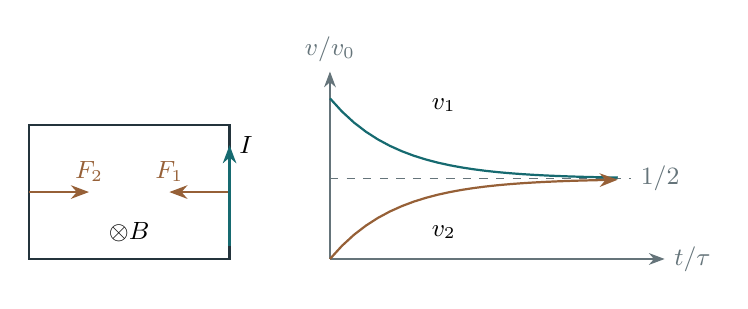
\begin{tikzpicture}[scale=.85]

\draw[object] (0,0) rectangle (3,2);\draw[force] (0,1)--(.9,1) node[above]{$F_2$};\draw[force] (3,1)--(2.1,1) node[above]{$F_1$};
\draw[motion] (3,.2)--(3,1.7);\node[right] at(3,1.7){$I$};\node at(1.5,.4){$\otimes B$};
\draw[axis] (4.5,0)--(9.5,0) node[right]{$t/\tau$};\draw[axis] (4.5,0)--(4.5,2.8) node[above]{$v/v_0$};
\draw[guide] (4.5,1.2)--(9,1.2) node[right]{$1/2$};
\draw[traj,domain=0:4.3] plot ({4.5+\x},{1.2*(1+exp(-\x))});
\draw[force,domain=0:4.3] plot ({4.5+\x},{1.2*(1-exp(-\x))});
\node at(6.2,2.3){$v_1$};\node at(6.2,.4){$v_2$};

\end{tikzpicture}\figcaption{解图电3.6A\quad 相反磁力使速度趋同；两条曲线之间的面积对应间距增加量。}\end{minipage}\end{center}

右棒电流向上，磁力向左；左棒电流向下，磁力向右。分别写运动方程：
\[
m\dot v_1=-B\ell I=-\frac{B^2\ell^2}{2R}(v_1-v_2),\qquad
m\dot v_2=+\frac{B^2\ell^2}{2R}(v_1-v_2).
\]
相加得$v_1+v_2=v_0$，即两棒总动量守恒。相减并令$u=v_1-v_2$：
\[
\dot u=-\frac{B^2\ell^2}{mR}u,\qquad
u(0)=v_0.
\]
定义$\tau=mR/(B^2\ell^2)$，积分得到
\[
u=v_0e^{-t/\tau},\quad
\boxed{v_1=\frac{v_0}{2}(1+e^{-t/\tau})},\quad
v_2=\frac{v_0}{2}(1-e^{-t/\tau}).
\]
两棒逐渐趋于共同速度$v_0/2$。速度差在全过程中按指数衰减，极限为零。

两根棒同时向右运动，右棒比左棒每秒多走 $u$，所以两棒的间距以 $\dot x=u$ 增加。由$x(0)=0$，有
\[
\boxed{x(t)=v_0\tau(1-e^{-t/\tau})},\qquad
\boxed{x_{\max}=\frac{mRv_0}{B^2\ell^2}}.
\]
解图电3.6A的速度曲线显示：地面位移各自仍可不断增加，而相对速度的时间积分有限，故间距有上限。由初末动能差还可求总焦耳热，得到
\[
Q=\frac12mv_0^2-2\frac12m\left(\frac{v_0}{2}\right)^2
=\frac14mv_0^2.
\]
直接积分$\int_0^\infty 2RI^2\dd t$也得同一热量。两棒间的磁力传递动量，随相对运动耗散的能量进入焦耳热。

相对运动与热量还可以按时间逐项分配。电流为
\[
I(t)=\frac{B\ell v_0}{2R}e^{-t/\tau},\quad
Q(t)=\int_0^t2RI^2\dd t'
=\frac{mv_0^2}{4}(1-e^{-2t/\tau}).
\]
以共同质心速度$v_0/2$分解总动能，得到
\[
K(t)=\underbrace{\frac{mv_0^2}{4}}_{K_{\rm cm}}
+\underbrace{\frac{mv_0^2}{4}e^{-2t/\tau}}_{K_{\rm rel}},
\qquad K(t)+Q(t)=\frac12mv_0^2.
\]

\begin{center}\begin{minipage}{.98\linewidth}\centering
\begin{tikzpicture}[scale=.85]

\draw[axis](0,0)--(5.5,0) node[right]{$t/\tau$};\draw[axis](0,0)--(0,3) node[above]{能量$/K_0$};
\draw[traj,domain=0:4.6,samples=60] plot ({\x},{1.2*(1+exp(-2*\x))});
\draw[force,domain=0:4.6,samples=60] plot ({\x},{1.2*(1-exp(-2*\x))});
\draw[guide](0,1.2)--(4.8,1.2);\node[left] at(0,1.2){$1/2$};\node[left] at(0,2.4){$1$};
\node at(1.2,2.1){$K/K_0$};\node at(1.7,.65){$Q/K_0$};
\node[align=left] at(8,1.6){$K_0=mv_0^2/2$\\$K_{\rm cm}=K_0/2$不变\\$K_{\rm rel}$转为热量};

\end{tikzpicture}\figcaption{解图电3.6B\quad 总动能趋于质心动能；曲线相加恒为初动能，热量来自相对运动。}\end{minipage}\end{center}

解图电3.6B显示热量来自相对运动动能，质心平移动能保持不变。初期$t\ll\tau$时，$v_1\simeq v_0(1-t/(2\tau))$、$v_2\simeq v_0t/(2\tau)$，因而$x\simeq v_0t$。右棒和左棒在 $t=0$ 的加速度分别为 $-v_0/(2\tau)$ 和 $v_0/(2\tau)$。

\begin{center}\begin{minipage}{.97\linewidth}\centering
\begin{tikzpicture}[x=4cm,y=2.6cm,font=\small]
\draw[axis] (0,0)--(1.22,0) node[right] {$x/(v_0\tau)$};\draw[axis] (0,0)--(0,1.25) node[above] {$u/v_0$};
\draw[traj,->] (0,1)--(.6,.4);\draw[traj] (.6,.4)--(1,0);\draw[fill=white] (1,0) circle(.8pt);
\node[left] at (0,1) {$1$};\node[below] at (1,0) {$1$};
\node[right] at (1.15,.8) {$u=v_1-v_2$};\node[right] at (1.15,.48) {$x/\tau+u=v_0$};
\node[right] at (1.15,.16) {空心点仅在$t\to\infty$到达};
\end{tikzpicture}
\figcaption{解图电3.6C　消去时间后的实际相对运动轨迹。相对速度为正使间距单调增加；空心端点是无限长导轨上 $t\to\infty$ 的间距极限。}
\end{minipage}\end{center}

\textbf{速度随间距的变化。} 由图A左棒的牛顿方程与$\dd x=(v_1-v_2)\dd t$，可直接消去时间：
\[
m\,\dd v_2=\frac{B^2\ell^2}{2R}\,\dd x,
\qquad x=\frac{2mR}{B^2\ell^2}v_2=2\tau v_2.
\]
初始$v_2=x=0$决定积分常量；再由$v_1+v_2=v_0$，得到
$v_1=v_0-x/(2\tau)$、$v_2=x/(2\tau)$以及$u=v_0-x/\tau$。
让$v_2$趋$v_0/2$即得到$x_{\max}$。因此解图电3.6C以间距变化作横轴时得到直线，图A以时间作横轴时则得到指数曲线。

上述过程还给完整反馈：右棒减速后其向上电动势降低，左棒加速后反向电动势增加，二者都使净电动势减小。
同一电流产生大小相等、方向相反的两磁力；合力为零只保住总动量，单根棒的动量仍在改变。
相对速度越小，电流和两力也越小。对于有限 $t$，$u=v_0e^{-t/\tau}$ 保持正值，因此间距单调趋于上限。两根棒各自的地面位移则持续增长，其中均含共同的平移项 $v_0 t/2$。

安培力对两根棒的总功率为
\[
F_1v_1+F_2v_2=-B\ell I(v_1-v_2)=-2RI^2.
\]
这说明右棒损失动能的一部分增加左棒动能，剩余变为焦耳热。
图B中保持不变的质心动能与衰减的相对动能分别有明确对象：前者属于系统共同平移，后者才是电磁耗散能够消除的运动。

时间常数适用于 $R>0$、$B\ne0$。若 $B=0$，两棒各以初速运动，间距增量为 $v_0t$。在固定观察时长内增大 $R$，$t/\tau$ 减小，速度逐渐接近各自初值。对任一有限 $R$，充分长的时间仍可使两棒趋向共同末速。若保留回路自感，电流还具有建立过程，小电阻时应在短时响应方程中保留这一项。


\Needspace{13\baselineskip}

\pdfbookmark[2]{第 7 题 强磁场中下落薄圆盘的电磁惯性}{q7}

\section*{第 7 题\quad 强磁场中下落薄圆盘的电磁惯性}\label{q:7}

半径为$R$、厚度为$D$的金属薄圆盘，盘面竖直，匀强磁场$B$沿水平方向且平行于盘面。圆盘由静止自由下落，密度$\rho=9.0\times10^3\,\mathrm{kg/m^3}$，电阻率视为零，忽略空气阻力和边缘效应，$D\ll R$。求使下落加速度较$g$减小$0.1\%$所需磁感应强度的数量级。取$\varepsilon_0=8.85\times10^{-12}\,\mathrm{F/m}$。

\begin{center}\begin{minipage}{.98\linewidth}\centering
\begin{tikzpicture}[scale=.85]

\draw[object] (0,0) circle(1.5);\draw[axis] (0,0)--(1.05,1.05) node[midway,above left]{$R$};
\draw[motion] (-2,0)--(2.1,0) node[right]{$B$};\draw[motion] (0,-1.8)--(0,-2.8) node[right]{$v,a$};
\node at(4.5,1){盘面竖直，厚度$D$};\node at(4.5,-.7){$B,v$均在盘面内};

\end{tikzpicture}\figcaption{图电3.7\quad 正视圆盘；电荷分离沿垂直盘面的厚度方向。}\end{minipage}\end{center}

\Needspace{6\baselineskip}\subsection*{解答}

图电3.7中，速度与磁场都在盘面内，$\vect v\times\vect B$沿盘的厚度方向。按解图电3.7A取速度向下、磁场向纸外，$\vect v\times\vect B$ 指向剖面左侧。左面带正电，内电场向右；零电阻近似下，盘内电荷满足 $\vect E+\vect v\times\vect B=0$。两表面间的电势差大小为
\[
U=BDv.
\]
将两表面近似为平行板，面积$A=\pi R^2$，电容为$C=\varepsilon_0 A/D$，故单个表面电荷量的绝对值为
\[
Q=CU=\varepsilon_0 ABv.
\]

\begin{center}\begin{minipage}{.98\linewidth}\centering
\begin{tikzpicture}[scale=.85]

\draw[object] (0,0) rectangle (.8,3);\foreach \y in {.4,1.2,2,2.7}{\node at(.1,\y){$+$};\node at(.7,\y){$-$};}
\draw[<->] (0,-.4)--(.8,-.4) node[midway,below]{$D$};
\draw[force] (.15,1.5)--(.65,1.5) node[above]{$E$};\draw[motion] (-1.8,2.5)--(-1.8,.8) node[left]{$v,a$};
\draw[force] (1.4,.8)--(1.4,2.6) node[right]{$F_B=IDB$};
\node at(.4,3.5){厚度剖面};\node at(4.8,3.3){$\odot B$};
\draw[motion] (.65,2.35)--(.15,2.35) node[left,xshift=-3pt]{$I=\dot Q$};
\node[align=left] at(4,.2){$U=BDv$\\$Q=\varepsilon_0\pi R^2Bv$};

\end{tikzpicture}\figcaption{解图电3.7A\quad 剖面取磁场向外；电流由负面向正面充电，磁力向上。}\end{minipage}\end{center}

圆盘在加速，表面电荷还在继续增加。解图电3.7A中穿过厚度的充电电流大小为
\[
I=\dot Q=\varepsilon_0 AB\dot v=\varepsilon_0 ABa.
\]
这个电流在磁场中受到向上的安培力。受力导电长度为厚度$D$，所以
\[
F_B=IDB=\varepsilon_0 ADB^2a.
\]
圆盘质量$m=\rho AD$。以下落方向为正，牛顿定律给出
\[
\rho ADa=\rho ADg-\varepsilon_0 ADB^2a,
\qquad
\boxed{a=\frac{g}{1+\varepsilon_0 B^2/\rho}}.
\]
要求$a=0.999g$，应保留加速度出现在安培力中的这一关系：
\[
B=\sqrt{\frac{\rho}{\varepsilon_0}\left(\frac1{0.999}-1\right)}
\simeq1.01\times10^6\,\mathrm T.
\]
所以所需磁场约为$10^6\,\mathrm T$。圆盘面积和厚度在比值中消去。

这里的阻碍作用由充电电流产生。圆盘匀速时$\dot Q=0$，该安培力也为零；它在这个理想模型中相当于增加了惯性质量$m_{\rm em}=\varepsilon_0 B^2AD$。电场能
\[
W_E=\tfrac12CU^2=\tfrac12\varepsilon_0 ADB^2v^2
\]
随速度增加，且$mgv=\dd(mv^2/2+W_E)/\dd t$，与受力式相符。这个数量级来自非相对论、均匀场和平行板近似，按题给的密度与零电阻取值计算。

用$\delta=(g-a)/g$表示相对减速，可把求场强的步骤写成
\[
\delta=\frac{\beta}{1+\beta},\qquad
\beta=\frac{\varepsilon_0B^2}{\rho}=\frac{\delta}{1-\delta}.
\]
本题$\delta=10^{-3}$，因而$\beta=1.0010\times10^{-3}$。在小减速比例下 $\beta=\delta+O(\delta^2)$，以首项代入同样得到 $10^6\,\mathrm T$ 的数量级。由于受力式中$a$是常量，由静止释放后$v=at$、下落高度$h=at^2/2$，并有
\[
mgh=\frac12(m+\varepsilon_0B^2AD)v^2.
\]
右端的第二部分正是两表面电场能。表面电荷正比于$t$增加，充电电流恒定。重力和向上的充电磁力均是常量，因而下落速度随时间线性增加。

\begin{center}\begin{minipage}{.97\linewidth}\centering
\begin{tikzpicture}[x=1cm,y=1cm,font=\small]
\draw[object] (0,0) rectangle(1.5,1.4);\node at (.75,.7) {$m=\rho AD$};
\draw[force] (.35,.7)--(.35,-1.2) node[below] {$mg$};
\draw[force] (1.15,.7)--(1.15,2.8) node[above] {$F_B=m_{\rm em}a$};
\draw[motion] (2.2,1)--(2.2,-.7) node[below] {$v,a$};
\node[align=left] at (5.7,1.2) {$m_{\rm em}=\varepsilon_0ADB^2$\\$(m+m_{\rm em})a=mg$\\匀速时充电电流为0};
\end{tikzpicture}
\figcaption{解图电3.7B　圆盘整体的受力，箭头仅标方向。上向磁力正比于加速度，移到惯性项后得到有效质量。}
\end{minipage}\end{center}
\begin{center}\begin{minipage}{.97\linewidth}\centering
\begin{tikzpicture}[x=1.6cm,y=2.5cm,font=\small]
\draw[axis] (0,0)--(3.3,0) node[right] {$\beta=\varepsilon_0B^2/\rho$};\draw[axis] (0,0)--(0,1.2) node[above] {比例};
\draw[traj,domain=0:3,samples=80,variable=\t] plot(\t,{1/(1+\t)});
\draw[thick,warm,domain=0:3,samples=80,variable=\t] plot(\t,{\t/(1+\t)});
\draw[guide] (0,.5)--(3,.5);\node[left] at (0,1) {$1$};
\node[right,accent] at (3.2,.27) {$a/g=1/(1+\beta)$};
\node[right,warm] at (3.2,.76) {$W_E/(mgh)=\beta/(1+\beta)$};
\end{tikzpicture}
\figcaption{解图电3.7C　所用理想模型的精确比例曲线。由静止下落同一非零高度h时，机械动能占重力功的比例为$a/g$，其余为电场能；本题处于$\beta\ll1$的一端。}
\end{minipage}\end{center}

解图电3.7B 先用充电电流求磁力，再把与加速度成正比的磁力项移到牛顿方程的惯性项一侧，得到有效质量。两个表面的电荷为 $+Q,-Q$，它们来自同一次厚度方向的电荷转移。$Q$ 增加 $\dd Q$ 时，穿过任一厚度截面的输运电量为 $\dd Q$，由这一电流求磁力。
电流路径贯穿盘厚，所以安培力公式中的导电长度为 $D$。

图A中电场向右而正充电电流向左，电流受到向上的磁力；已经建立的表面电荷仍随盘整体下落，但两个表面的平移磁力在总力中抵消。
充电时，正电荷的净输运经过厚度方向，额外产生大小为 $B D\dot Q$ 的向上磁力。

在同一高度差 $h$ 内，解图电3.7C的两条曲线分别给重力功进入动能和电场能的比例：
\[
\frac{K}{mgh}=\frac{m}{m+m_{\rm em}}=1-\delta,\qquad
\frac{W_E}{mgh}=\frac{m_{\rm em}}{m+m_{\rm em}}=\delta.
\]
所以题给千分之一的加速度变化，也对应这一模型中重力功的千分之一进入电场能。
这部分是可恢复储能；若使速度减小，充电电流反向，磁力也反向，反作用始终与加速度相反。电场释放储能时，磁力沿原下落方向。


\Needspace{13\baselineskip}

\pdfbookmark[2]{第 8 题 随动电压表与圆弧导体的端点电势}{q8}

\section*{第 8 题\quad 随动电压表与圆弧导体的端点电势}\label{q:8}

一块沿$x$方向无限长、宽为$L$的静止金属板电阻可忽略。半径$L/\sqrt2$的圆弧导体$aebcfd$沿板的长边以速度$v$滑动，圆弧平面垂直$x$轴，$a,d$始终接触板的两条边。正视图中$a,b,c,d$是圆上内接正方形的左下、左上、右上、右下顶点，$e,f$为圆的最左、最右点；$ae,eb,cf,fd$各为八分之一圆弧、电阻均为$R/2$，$bc$为四分之一圆弧、电阻为$R$。匀强磁场$B$竖直向上。电阻$R_V=nR$的电压表位于圆心$O$，由理想径向导线连接$b,c$，并随圆弧一起运动，$n>0$。求电压表读数及静电势差$U_e-U_f$。

\begin{center}\begin{minipage}{.98\linewidth}\centering
\begin{tikzpicture}[scale=.85]

\draw[guide] (-1.5,-1.5)--(1.5,-1.5);\draw[object] (-1.5,-1.5) arc(225:-45:2.1213);
\draw[object] (-1.5,1.5)--(0,0)--(1.5,1.5);\draw[fill=white] (0,0) circle(.23) node{$V$};
\foreach \x/\y/\lab/\pos in {-1.5/-1.5/a/below left,-1.5/1.5/b/above left,1.5/1.5/c/above right,1.5/-1.5/d/below right,-2.121/0/e/left,2.121/0/f/right}{\fill (\x,\y) circle(1.2pt) node[\pos]{$\lab$};}
\draw[object] (-1.5,-1.5)--(-.4,-2.5)--(2.6,-2.5)--(1.5,-1.5);\node at(1.1,-2.8){静止金属板，沿$x$延伸};
\draw[<->] (-1.5,-1.9)--(1.5,-1.9) node[midway,below]{$L$};
\draw[motion] (3.3,-.7)--(3.3,1.8) node[above]{$B$};\node at(4.7,.3){$\odot\ v(+x)$};
\draw[axis] (3,-2)--(5,-2) node[right]{$y$};

\end{tikzpicture}\figcaption{图电3.8\quad 正视圆弧，板的延伸用斜线示意；径向引线和表头随弧运动。}\end{minipage}\end{center}

\Needspace{6\baselineskip}\subsection*{解答}

取正视图向右为$y$、向上为$z$，运动方向为$+x$，于是$\vect v\times\vect B=-Bv\vect e_y$。沿任一随动导体段，由$p$到$q$的动生电动势为$-Bv(y_q-y_p)$；它等于沿横向的有向投影乘 $-Bv$。

\begin{center}\begin{minipage}{.98\linewidth}\centering
\begin{tikzpicture}[scale=.85]

\draw[object] (0,0)--(0,3)--(4.5,3)--(4.5,0);
\draw[object] (0,3)--(1,2)--(3.5,2)--(4.5,3);\node[fill=white] at(2.25,3){$R$};\node[fill=white] at(2.25,2){$nR$};
\node[above left] at(0,3){$b$};\node[above right] at(4.5,3){$c$};\node[fill=white] at(0,.8){$R$};\node[fill=white] at(4.5,.8){$R$};
\node[below] at(0,0){$a$};\node[below] at(4.5,0){$d$};\fill (0,1.5) circle(1.5pt) node[left]{$e$};\fill (4.5,1.5) circle(1.5pt) node[right]{$f$};
\node[align=left] at(7.1,2.1){$\chi=U+Bvy$\\$\chi_d-\chi_a=BLv$\\中央两条路径并联};
\node[align=left] at(7.1,.3){$y_f-y_e=\sqrt2L$\\表读数用$\chi$差\\静电势须还原$U$};

\end{tikzpicture}\figcaption{解图电3.8A\quad 辅助势网络：两外侧$R$串联中央的$R\parallel nR$；几何端点与题图相同。}\end{minipage}\end{center}

解图电3.8A中引入随动支路的辅助量
\[
\chi=U+Bvy.
\]
沿$p\to q$，欧姆定律成为$I_{pq}R_{pq}=\chi_p-\chi_q$。静止板使$U_a=U_d$，取二者为零。由于$y_a=-L/2,y_d=L/2$，有
\[
\chi_a=-\frac{BLv}{2},\quad \chi_d=\frac{BLv}{2},\quad
\chi_d-\chi_a=\mathcal E_0=BLv.
\]
因此在$\chi$网络中，$ab$段和$cd$段各为$R$，中间$b,c$之间有电阻$R$与$nR$并联。两段外侧支路电流大小相同，记$I_1$；$bc$圆弧和表头的电流分别为$I_2,I_3$。从$d$经$c,b$到$a$列式：
\[
I_1=I_2+I_3,\qquad I_2R=I_3nR,\qquad
2I_1R+I_3nR=\mathcal E_0.
\]
代入$I_2=nI_3,I_1=(n+1)I_3$，得到
\[
I_3=\frac{\mathcal E_0}{(3n+2)R},\quad
I_1=\frac{(n+1)\mathcal E_0}{(3n+2)R},\quad
I_2=\frac{n\mathcal E_0}{(3n+2)R}.
\]
随动表头读数是其电阻上的压降，即
\[
\boxed{V=I_3nR=\frac{n}{3n+2}BLv}.
\]
这个压降是 $\chi_c-\chi_b$。两条径向引线一起随圆弧滑动，从弧端到表头的静电势变化包含各自的动生电动势。

在$e\to b\to c\to f$路径上，电流由$f$向$e$，所以
\[
\chi_f-\chi_e=I_1\frac R2+I_2R+I_1\frac R2
=\frac{2n+1}{3n+2}\mathcal E_0.
\]
又有$y_f-y_e=\sqrt2L$，将$\chi$还原为静电势：
\[
\boxed{U_e-U_f=\left(\sqrt2-\frac{2n+1}{3n+2}\right)BLv}.
\]
当 $n\to\infty$，表头电流趋零，表两端的辅助势差趋于 $BLv/3$。外侧圆弧和中央圆弧串联，三个等值电阻各分得 $\mathcal E_0/3$，所以 $U_e-U_f$ 趋于 $(\sqrt2-2/3)BLv$。

将表头端点移到圆心附近，可以看清读数为何使用$\chi$。理想径向引线无电阻，故各自满足$\Delta\chi=0$；设其靠近表头的端点为$O_b,O_c$，两点的$y$坐标均近于零，则
\[
U_{O_b}=\chi_b,\quad U_{O_c}=\chi_c,\quad
V=|U_{O_c}-U_{O_b}|=|\chi_c-\chi_b|.
\]
相反，圆弧顶点的静电势差为
\[
U_b-U_c=\chi_b-\chi_c+Bv(y_c-y_b)
=\frac{2(n+1)}{3n+2}BLv.
\]

\begin{center}\begin{minipage}{.98\linewidth}\centering
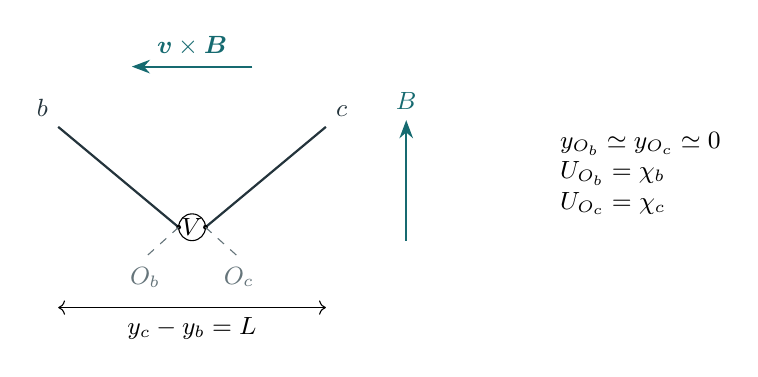
\begin{tikzpicture}[scale=.85]

\draw[object](-2,1.5) node[above left]{$b$}--(-.2,0) (.2,0)--(2,1.5) node[above right]{$c$};
\draw[fill=white](0,0) circle(.2) node{$V$};\fill(-.2,0) circle(1pt);\fill(.2,0) circle(1pt);
\draw[guide](-.2,0)--(-.7,-.45) node[below]{$O_b$};\draw[guide](.2,0)--(.7,-.45) node[below]{$O_c$};
\draw[<->](-2,-1.2)--(2,-1.2) node[midway,below]{$y_c-y_b=L$};
\draw[motion](.9,2.4)--(-.9,2.4) node[midway,above]{$\vect v\times\vect B$};
\draw[motion](3.2,-.2)--(3.2,1.6) node[above]{$B$};
\node[align=left] at(6.7,.8){$y_{O_b}\simeq y_{O_c}\simeq0$\\$U_{O_b}=\chi_b$\\$U_{O_c}=\chi_c$};

\end{tikzpicture}\figcaption{解图电3.8B\quad 两引线随动且无电阻，保持各自的辅助势；表头两端是不同接点。}\end{minipage}\end{center}

解图电3.8B把两条径向引线的横向投影分别标出。它们把$b,c$的电势带到圆心时，沿途的动生电动势也进入测量，因此表头读数与$U_b-U_c$不同。利用 $e,f$ 分别位于两侧等阻分段的接点，由相等的外侧电阻分段，$\chi_e=(\chi_a+\chi_b)/2$、$\chi_f=(\chi_d+\chi_c)/2$，于是$\chi_f-\chi_e=(\mathcal E_0+V)/2$，代回即得到前述$U_e-U_f$。

\begin{center}\begin{minipage}{.97\linewidth}\centering
\begin{tikzpicture}[x=.75cm,y=2.6cm,font=\small]
\draw[axis] (0,0)--(6.8,0) node[below right] {$n=R_V/R$};\draw[axis] (0,0)--(0,1.2) node[above] {势差$/\mathcal E_0$};
\draw[traj,domain=0:6,samples=90,variable=\t] plot(\t,{\t/(3*\t+2)});
\draw[thick,warm,domain=0:6,samples=90,variable=\t] plot(\t,{2*(\t+1)/(3*\t+2)});
\draw[guide] (0,.3333333)--(6.2,.3333333);\draw[guide] (0,.6666667)--(6.2,.6666667);
\node[left] at (0,1) {$1$};\node[left] at (0,.3333333) {$1/3$};\node[left] at (0,.6666667) {$2/3$};
\node[right,warm] at (6.5,.85) {$(U_b-U_c)/\mathcal E_0$};
\node[right,accent] at (6.5,.4) {$V/\mathcal E_0$};
\node[right] at (6.5,.16) {两曲线之和恒为1};
\end{tikzpicture}
\figcaption{解图电3.8C　随动表头读数与圆弧端点静电势差的实际负载曲线。两者互补，$n\to\infty$时分别趋$1/3$与$2/3$；$n=0$按短接极限理解。}
\end{minipage}\end{center}

在解图电3.8A左侧，圆弧及引线各段的横向投影给相应的动生电动势。
圆半径为$L/\sqrt2$，故$ae,eb,cf,fd$每段横向投影的绝对值均为$(\sqrt2-1)L/2$，
每段动生电动势大小为$e_s=(\sqrt2-1)\mathcal E_0/2$；$bc$投影为L，电动势大小为$\mathcal E_0$。
两条径向引线的投影各为$L/2$，各自电动势大小为$\mathcal E_0/2$。
这些值要按路径方向带符号；例如从$f$经$c$到$b$再到e，总投影向左，动生作用与反方向路径不同号。

在完整电源网络中，中央圆弧与“引线—表头—引线”两条$b,c$路径同速运动，端点也相同，故动生电动势的代数和相等。
两支路的动生电动势相同，减去共同项便得到 $I_2R=I_3nR$。
外侧四个八分之一圆弧电阻总和为$2R$，与中央表头支路共同构成的式子则是$2I_1R+I_3nR=\mathcal E_0$。
辅助势把各段动生电动势的累加包含进端点差，直接得到同一组支路方程。

解图电3.8C同时画两种位置的电压关系，所有$n>0$均有$V+(U_b-U_c)=\mathcal E_0$。
表头在圆心，两个表端横向坐标近乎相同，读数可按两端静电势差取得；b、c却相隔L，
沿引线换算到弧端时，按两端的投影距离 $L$ 加上动生项。随动弧段用 $\chi$ 写电阻压降；静止板的两端则有相等的静电势 $U$。


\Needspace{13\baselineskip}

\pdfbookmark[2]{第 10 题 磁流体发电机的流速反馈}{q10}

\section*{第 10 题\quad 磁流体发电机的流速反馈}\label{q:10}

矩形管道长为$\ell$，截面宽$a$、高$b$。上下壁绝缘，两侧电极电阻不计并接外电阻$R_L$。电阻率$\rho_e$的导电流体沿管以均匀速度$v$流动，竖直匀强磁场$B$垂直上下壁。管道两端固定压强差为$P$，流体机械阻力为$\alpha v$；没有磁场时稳态流速为$v_0$。忽略端部效应，求加上磁场后的感应电动势，并说明负载端电压与它的关系。

\begin{center}\begin{minipage}{.98\linewidth}\centering
\begin{tikzpicture}[scale=.85]

\draw[object] (0,0) rectangle (5,2);\draw[object] (0,2)--(1,3)--(6,3)--(6,1)--(5,0) (5,2)--(6,3);
\draw[object] (0,0)--(1,1)--(6,1);\draw[guide] (1,1)--(1,3);
\draw[motion] (1,1.4)--(4,1.4) node[midway,below]{$v$};\draw[motion] (3,2.6)--(3,4) node[above]{$B$};
\node[above] at(2.5,3){$\ell$};\node[right] at(6,2){$b$};\node[below right] at(5.5,.5){$a$};
\draw[object] (2.5,0)--(2.5,-.8)--(6.8,-.8)--(6.8,2)--(5.5,2.5);\node[fill=white] at(4.3,-.8){$R_L$};
\node at(0,3.8){高压端};\node at(6.3,3.8){低压端};

\end{tikzpicture}\figcaption{图电3.10\quad 流向沿管长，电流横穿宽$a$，电极接外负载。}\end{minipage}\end{center}

\Needspace{6\baselineskip}\subsection*{解答}

图电3.10中电流横穿宽度$a$，导电截面积是$b\ell$，因此流体的内电阻及动生电动势为
\[
R_i=\rho_e\frac{a}{b\ell},\qquad \mathcal E=Bav,\qquad
I=\frac{Bav}{R_L+R_i}.
\]
没有磁场时，压强差产生的推力$Pab$与机械阻力平衡，故$\alpha=Pab/v_0$。接上有限负载后，横向电流在磁场中产生逆流向的安培力，流速由两种阻力共同决定。

\begin{center}\begin{minipage}{.98\linewidth}\centering
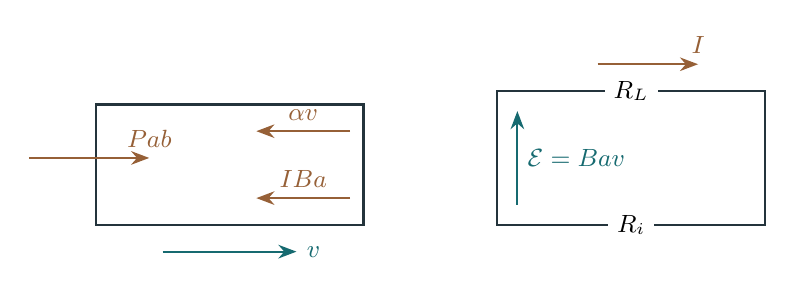
\begin{tikzpicture}[scale=.85]

\draw[object] (0,0) rectangle(4,1.8);\draw[force] (-1,1)--(.8,1) node[above]{$Pab$};
\draw[force] (3.8,1.4)--(2.4,1.4) node[midway,above]{$\alpha v$};\draw[force] (3.8,.4)--(2.4,.4) node[midway,above]{$IBa$};
\draw[motion] (1,-.4)--(3,-.4) node[right]{$v$};
\draw[object] (6,0) rectangle (10,2);\node[fill=white] at(8,2){$R_L$};\node[fill=white] at(8,0){$R_i$};
\draw[motion] (6.3,.3)--(6.3,1.7) node[midway,right]{$\mathcal E=Bav$};\draw[force] (7.5,2.4)--(9,2.4) node[above]{$I$};

\end{tikzpicture}\figcaption{解图电3.10A\quad 流向受力与带内阻发电回路共同决定稳态流速。}\end{minipage}\end{center}

解图电3.10A中，这个磁阻力大小为$F_B=IBa$。写流向的稳态受力式，记$R_\Sigma=R_L+R_i$：
\[
Pab=\alpha v+IBa
=\frac{Pab}{v_0}v+\frac{B^2a^2}{R_\Sigma}v.
\]
整理得到
\[
v=\frac{v_0}{1+B^2av_0/(PbR_\Sigma)},
\qquad
\boxed{\mathcal E=\frac{Bav_0}{1+B^2av_0/[Pb(R_L+\rho_e a/(b\ell))]}}.
\]
外负载端电压还要扣除流体内阻上的压降：
\[
\boxed{U_L=\frac{R_L}{R_L+R_i}\mathcal E},\qquad P_L=I^2R_L.
\]
受力式乘$v$得到功率平衡
\[
Pabv=\alpha v^2+I^2(R_L+R_i).
\]
左边是维持压强差的装置提供的机械功率，右边分别为流体机械耗散、外电阻热和流体内部电热。开路$R_L\to\infty$时$I\to0,v\to v_0$；短路时$U_L=0$，但$R_i$有限仍有电流和磁阻力，此时动生电动势全部分配到流体内阻。

在解图电3.10B的横截面上，电流沿宽度 $a$ 穿过流体。流体沿$+x$流出纸面，$B$向上，正电荷在$\vect v\times\vect B$作用下趋向左电极，流体内电流向左，磁力沿$-x$，恰与流动相反。

\begin{center}\begin{minipage}{.98\linewidth}\centering
\begin{tikzpicture}[scale=.8]

\draw[guide](0,0)--(4,0) (0,2.4)--(4,2.4);\draw[force,very thick](0,0)--(0,2.4);\draw[traj,very thick](4,0)--(4,2.4);
\node[above left] at(0,2.4){$+$};\node[above right] at(4,2.4){$-$};
\draw[force](3.3,1.2)--(.7,1.2) node[midway,above]{$I$};\node at(2,.45){$\odot v$};
\draw[motion](2,1.8)--(2,3.2) node[above]{$B$};
\draw[object](0,1.2)--(-.8,1.2)--(-.8,-1.3)--(4.8,-1.3)--(4.8,1.2)--(4,1.2);\node[fill=white] at(2,-1.3){$R_L$};
\draw[force](1,-1.8)--(3,-1.8) node[midway,below]{$I$};
\draw[<->](0,-.45)--(4,-.45) node[midway,below]{$a$};\draw[<->](5.2,0)--(5.2,2.4) node[midway,right]{$b$};
\node[align=left] at(7.5,1.2){截面法线$+x$向外\\磁力$F_B$沿$-x$\\$R_i=\rho_e a/(b\ell)$};

\end{tikzpicture}\figcaption{解图电3.10B\quad 横截面中电流向左；它在竖直磁场中受向里的力，与流动相反。}\end{minipage}\end{center}

稳态受力式还可以直接改写为电流与负载的关系：
\[
v=v_0\left(1-\frac{IB}{Pb}\right),\quad
\mathcal E=Bav_0-I\frac{B^2av_0}{Pb}.
\]
定义$\mathcal E_{\rm oc}=Bav_0$、$R_g=B^2av_0/(Pb)$，则
\[
I=\frac{\mathcal E_{\rm oc}}{R_L+R_i+R_g},\qquad
U_L=\frac{R_L\mathcal E_{\rm oc}}{R_L+R_i+R_g}.
\]
$R_g$ 是电流使流速降低以后，引起的电动势降量与电流之比。它与实际的流体内阻 $R_i$ 一起决定端电压对电流的斜率。实际发热仍由流体及外接电阻给出。求最大负载功率时，应用整个端口的内电阻 $R_i+R_g$。

\begin{center}\begin{minipage}{.97\linewidth}\centering
\begin{tikzpicture}[x=1cm,y=3cm,font=\small]
\draw[axis](0,0)--(5.4,0) node[below right]{$x=R_L/(R_i+R_g)$};
\draw[axis](0,0)--(0,1.2) node[above]{归一化量};
\draw[traj,domain=0:5,samples=100,variable=\t]plot(\t,{\t/(1+\t)});
\draw[thick,warm,domain=0:5,samples=100,variable=\t]plot(\t,{4*\t/(1+\t)^2});
\draw[guide](1,0)--(1,1);\node[below]at(1,0){$1$};\node[left]at(0,1){$1$};
\node[right,warm]at(5.5,.98){$P_L/P_{\max}$};\node[right,accent]at(5.5,.7){$U_L/\mathcal E_{\rm oc}$};
\end{tikzpicture}
\figcaption{解图电3.10C　定压时的实际负载曲线。端电压随负载电阻增大而上升，输出功率在$R_L=R_i+R_g$最大。}
\end{minipage}\end{center}

解图电3.10C使用的横轴含机械反馈电阻。由前述端口式逐步得到
\[
P_L=\frac{\mathcal E_{\rm oc}^2R_L}{(R_L+R_i+R_g)^2},\quad
\frac{\dd P_L}{\dd R_L}=\mathcal E_{\rm oc}^2\frac{R_i+R_g-R_L}{(R_L+R_i+R_g)^3}.
\]
导数由正变负，故$P_{\max}=\mathcal E_{\rm oc}^2/[4(R_i+R_g)]$。
图中电压曲线为$x/(1+x)$，功率曲线为$4x/(1+x)^2$。工作点$x=1$处端电压是开路电压的一半。用 $I_*$ 代入流向受力式，流速为
\[
v_*=v_0\frac{2R_i+R_g}{2(R_i+R_g)}.
\]
当 $R_i>0$ 时，这一流速大于 $v_0/2$。固定负载而改变磁场时，图 A 的磁阻力与机械阻力之比为 $B^2a^2/[\alpha(R_L+R_i)]$。两种阻力相等时，压强推力的一半分配给机械阻力，流速为 $v_0/2$。

把解图电3.10B沿管长分成许多窄片。厚为 $\dd x$ 的一片中，横向电流穿过长度 $a$，相应的导电截面为 $b\dd x$；各片并接成总横截面 $b\ell$。每片的磁力是 $Ba\,\dd I$，求和得 $IBa$。压力功率等于压强差乘体积流量 $P(abv)$。其中 $\alpha v^2$ 消耗于机械阻力，另外两项 $I^2R_i$ 和 $I^2R_L$ 分别在流体内与负载上发热。


\Needspace{13\baselineskip}

\pdfbookmark[2]{第 11 题 双辐条轮的电磁传动与效率}{q11}

\section*{第 11 题\quad 双辐条轮的电磁传动与效率}\label{q:11}

两个相同金属轮各有四根长为$\ell$的径向辐条，每根电阻为$r$，轮轴、轮缘及接触电刷的电阻忽略。两轴电连接，两轮缘也电连接，轮面处于同一垂直纸面向里的匀强磁场$B$中。第一轮由外力维持角速度$\omega_1$；第二轮起初静止，转动时轮缘受大小恒为$F$的切向阻力。忽略电路自感，设第二轮能够启动并最终稳定转动。求其稳态角速度$\omega_2$、维持第一轮转动所需的外加功率及电磁传动效率，并讨论能够稳定同向转动的条件。

\begin{center}\begin{minipage}{.98\linewidth}\centering
\begin{tikzpicture}[scale=.85]

\foreach \c/\lab in {0/1,5/2}{\begin{scope}[xshift=\c cm]
\draw[object] (0,0) circle(1.4);\foreach \ang in {0,90,180,270}{\draw[object] (0,0)--(\ang:1.4);}
\fill (0,0) circle(2pt);\node at(0,-1.9){轮$\lab$};\node at(.7,.7){$\otimes B$};\end{scope}}
\draw[object] (0,0)--(0,2.4)--(5,2.4)--(5,0);\node at(2.5,2.7){轴接轴};
\draw[object] (0,-1.4)--(0,-2.4)--(5,-2.4)--(5,-1.4);\node at(2.5,-2.7){缘接缘};
\draw[motion] (-1.8,1) arc(150:60:2) node[above]{$\omega_1$};\draw[force] (6.4,0)--(6.4,1) node[right]{$F$};

\end{tikzpicture}\figcaption{图电3.11\quad 四根辐条并联于轴与缘之间；轴引线跨过轮缘处绝缘，第二轮受切向阻力。}\end{minipage}\end{center}

\Needspace{6\baselineskip}\subsection*{解答}

一根辐条转动时，各半径处线速度为$\omega r'$。轴到轮缘的动生电动势大小为
\[
\mathcal E_i=\int_0^\ell B\omega_i r'\dd r'
=\frac12B\omega_i\ell^2.
\]
同一轮的四根辐条连接在同一轴、同一轮缘之间，是四个相同电源并联。其电动势仍为$\mathcal E_i$，等效内阻为$r/4$。

\begin{center}\begin{minipage}{.98\linewidth}\centering
\begin{tikzpicture}[scale=.85]

\draw[object] (0,0)--(2.3,0);\fill(0,0) circle(2pt) node[below]{轴};\draw[motion] (.15,0)--(.85,0) node[midway,above]{$I/4$};\node at(2.8,.45){$\otimes B$};\node[below] at(2.3,0){缘};
\draw[force] (1.4,0)--(1.4,1) node[above]{$\dd F=(I/4)B\dd r'$};\draw[<->] (0,-.5)--(1.4,-.5) node[midway,below]{$r'$};
\draw[object] (4,0) rectangle(10,2.3);\node[fill=white] at(7,2.3){$r/4+r/4$};
\draw[motion] (4.3,.3)--(4.3,1.9) node[midway,right]{$\mathcal E_1$};
\draw[motion] (9.7,1.9)--(9.7,.3) node[midway,left]{$\mathcal E_2$};
\node at(7,.8){$I=(\mathcal E_1-\mathcal E_2)/(r/2)$};

\end{tikzpicture}\figcaption{解图电3.11A\quad 左图取第一轮的一根辐条，磁力矩阻碍转动；右图保留第二轮反电动势。}\end{minipage}\end{center}

解图电3.11A中，两轮同向转动时电动势在外回路中相反。总电流由第一轮驱动第二轮，大小为
\[
I=\frac{\mathcal E_1-\mathcal E_2}{r/4+r/4}
=\frac{B\ell^2}{r}(\omega_1-\omega_2).
\]
每根辐条电流为$I/4$。一根辐条的安培力矩为$\int_0^\ell (I/4)Br'\dd r'=IB\ell^2/8$，四根合计
\[
\tau_B=\frac12IB\ell^2.
\]
第二轮稳定时，$\tau_B=F\ell$，从而
\[
I=\frac{2F}{B\ell},\qquad
\boxed{\omega_2=\omega_1-\frac{2Fr}{B^2\ell^3}}.
\]
带正负载稳定同向转动时，$0<\omega_2<\omega_1$ 对应
\[
0<F<F_c,\qquad F_c=\frac{B^2\ell^3\omega_1}{2r}.
\]
启动时，第二轮的反电动势为零，电磁力矩达到 $F_c\ell$。若有静摩擦，启动条件是它的最大阻力矩小于 $F_c\ell$。在恒定切向阻力模型里，$F=F_c$ 对应零转速临界值。

第一轮外力做功功率为$P_{\rm in}=\tau_B\omega_1=\mathcal E_1I$。第二轮克服阻力的有用功率为$P_{\rm out}=F\ell\omega_2=\mathcal E_2I$，所以
\[
\boxed{\eta=\frac{P_{\rm out}}{P_{\rm in}}=\frac{\omega_2}{\omega_1}
=1-\frac{2Fr}{B^2\ell^3\omega_1}}.
\]
两轮焦耳热功率$I^2r/2=F\ell(\omega_1-\omega_2)$，恰等于输入与输出之差。阻力很小时效率接近一，但有用功率也趋零，两者随负载大小的变化见解图电3.11C。

在一根辐条上，半径 $r^\prime$ 处的速度为 $\omega r^\prime$，微元机械功率为$\dd P=\omega r'\dd F$；四根相加积分给
\[
P_{\rm em}=\omega\int_0^\ell IBr'\dd r'
=\frac12IB\ell^2\omega=\mathcal EI.
\]
解图电3.11A左侧取第一轮向外的辐条电流，图示安培力产生逆其转动的力矩；第二轮电流反向，电磁力矩则驱动转动，二者力矩大小相同。稳态下把输出功率写成负载的函数，得
\[
P_{\rm out}=F\ell\omega_1\left(1-\frac F{F_c}\right),\quad
P_{\max}=\frac{F_c\ell\omega_1}{4}
=\frac{B^2\ell^4\omega_1^2}{8r}.
\]
最大输出发生在$F=F_c/2$、$\omega_2=\omega_1/2$，此时效率为$1/2$。这与轻载时效率趋于一、输出功率却趋零的极限相互补充。

\begin{center}\begin{minipage}{.97\linewidth}\centering
\begin{tikzpicture}[scale=.8,font=\small]
\draw[object](0,0)circle(1.7);\draw[object](0,0)--(1.7,0);\fill(0,0)circle(2pt)node[left]{轴};
\node[above]at(0,2.1){第二轮};\node at(-1,.7){$\otimes B$};
\draw[motion](1.4,.15)--(.45,.15)node[midway,above]{$I/4$};
\draw[force](.9,-.15)--(.9,-2.2)node[below]{$\dd F_B$};
\draw[force](1.7,0)--(1.7,1.25)node[right]{$F$};
\draw[motion](2.7,.5)--(2.7,-.7)node[right]{$v_{\text{缘}}$};
\node[align=left]at(6.3,.8){电流径向向内，磁力矩顺时针\\$\tau_B=IB\ell^2/2=F\ell$};
\node[align=left]at(6.3,-1){$P_{\rm in}=F\ell\omega_1$\\$P_{\rm out}=F\ell\omega_2$\\$P_J=F\ell(\omega_1-\omega_2)$};
\end{tikzpicture}
\figcaption{解图电3.11B　第二轮的一根辐条与轮缘负载。图示微元磁力驱动顺时针转动；轮缘阻力反向，两个力矩在稳态平衡。}
\end{minipage}\end{center}

解图电3.11B把第二轮的方向单独画出：在右侧辐条上电流径向向内，$\boldsymbol B$向里，故磁力向下，驱动顺时针转动。
轮缘阻力向上，力臂为 $\ell$。辐条微元磁力的力臂为 $r^\prime$，随积分位置改变。
第一轮同位置的电流径向向外，安培力向上，所以第一轮的外加力矩沿顺时针方向补偿电磁阻力矩。
外加功率由此明确为
\[
\boxed{P_{\rm in}=\frac12IB\ell^2\omega_1=F\ell\omega_1}.
\]
同一电流经过两个轮子的并联辐条网络，每根辐条电流均为$I/4$，八根真实电阻合计的发热为
\[
P_J=8\left(\frac I4\right)^2r=\frac12 I^2r
=(\mathcal E_1-\mathcal E_2)I=F\ell(\omega_1-\omega_2).
\]
第一轮输入功率 $P_{\rm in}$ 经回路分成两部分。第二轮的 $\mathcal E_2 I$ 在稳态下传给轮缘负载；两轮辐条造成的欧姆热为 $I^2r/2$。相加得 $P_{\rm out}+P_J=P_{\rm in}$。
\begin{center}\begin{minipage}{.97\linewidth}\centering
\begin{tikzpicture}[x=5cm,y=2.8cm,font=\small]
\draw[axis](0,0)--(1.1,0)node[below right]{$f=F/F_c$};\draw[axis](0,0)--(0,1.2)node[above]{比例};
\draw[traj](0,1)--(1,0);\draw[thick,warm,domain=0:1,samples=80,variable=\t]plot(\t,{4*\t*(1-\t)});
\draw[guide](.5,0)--(.5,1);\node[below]at(.5,0){$1/2$};\node[below]at(1,0){$1$};\node[left]at(0,1){$1$};
\node[right,warm]at(1.15,.95){$P_{\rm out}/P_{\max}$};\node[right,accent]at(1.15,.55){$\eta=\omega_2/\omega_1$};
\end{tikzpicture}
\figcaption{解图电3.11C　同一稳态负载范围内的效率与输出曲线。轻载效率趋于一而输出趋零，最大功率发生在半速处。}
\end{minipage}\end{center}

解图电3.11C的横轴仅画$0\le f\le1$，同向带载稳定转动对应 $0<f<1$。
每个工作点的电流由负载力矩决定，$I=2F/(B\ell)$；电路所需的电动势差则靠转速差提供。
有限负载需要正电流，第一轮因此保持较高转速。当两轮无负载且同步时，两电动势相消，输入与输出同时为零。图左端的 $\eta\to1$ 是从带载状态趋向 $f=0$ 的极限。
在$f=1$端，堵转时有电流和输入功率，输出为零，输入全部耗为八根辐条的焦耳热。
最大功率处$f=1/2$，输出与焦耳热各占输入一半。


\Needspace{13\baselineskip}

\pdfbookmark[2]{第 12 题 感生电场中的圆弧与三角形混合电路}{q12}

\section*{第 12 题\quad 感生电场中的圆弧与三角形混合电路}\label{q:12}

半径$a$的均匀圆形导线通过三个等分圆周的点$A,B,C$，每段三分之一圆弧的电阻为$r_1$。再用直导线连接三点，其中$AB,CA$各为$r_2$，$BC$为$2r_2$，且$2r_1=3r_2$。匀强磁场垂直纸面向里，以恒定速率$k>0$减小；感生电场关于圆心轴对称，忽略自感。$A,B,C$按顺时针排列，求静电势差$U_A-U_B$。

\begin{center}\begin{minipage}{.98\linewidth}\centering
\begin{tikzpicture}[scale=.85]

\draw[object] (0,0) circle(2);\draw[traj] (90:2) node[above]{$A$}--(-30:2) node[right]{$B$}--(210:2) node[left]{$C$}--cycle;
\node[above right] at(.9,.9){$r_2$};\node[above left] at(-.9,.9){$r_2$};\node[below] at(0,-1){$2r_2$};
\node at(4,1.5){圆弧各$r_1$};\node at(4,.3){$\otimes B$，减小};\fill(0,0) circle(1pt) node[below]{$O$};

\end{tikzpicture}\figcaption{图电3.12\quad 圆弧与直弦分别连接相同节点；两类路径的感生电动势不同。}\end{minipage}\end{center}

\Needspace{6\baselineskip}\subsection*{解答}

磁场向里且减小，感生电场沿顺时针方向。解图电3.12A中，一段三分之一圆弧的感生电动势为其所围扇形的磁通变化率；一条弦的电动势则由圆心与弦围成的三角形面积决定：
\[
e_1=\frac{\pi a^2k}{3},\qquad e_2=\frac{\sqrt3a^2k}{4}.
\]
两条经过圆心的径向段积分为零。相同端点的弦和圆弧围出的面积不同，感生电动势之差对应这块弓形。

\begin{center}\begin{minipage}{.98\linewidth}\centering
\begin{tikzpicture}[scale=.85]

\fill[accent!12] (0,0)--(90:2) arc(90:-30:2)--cycle;
\fill[warm!25] (0,0)--(90:2)--(-30:2)--cycle;
\draw[object] (0,0) circle(2);\draw[traj] (90:2) node[above]{$A$}--(-30:2) node[right]{$B$}--(210:2) node[left]{$C$}--cycle;
\draw[guide] (90:2)--(0,0)--(-30:2);\node at(-.3,.1){$O$};
\draw[motion] (70:2.3) arc(70:0:2.3) node[right]{$I_1,e_1$};
\draw[force] (.5,1.1)--(1.1,.1) node[midway,left]{$I_2,e_2$};
\node[align=left] at(6,1.1){扇形：$e_1=\pi a^2k/3$\\三角形：$e_2=\sqrt3a^2k/4$\\$IR=U_{\text{起}}-U_{\text{终}}+e$};

\end{tikzpicture}\figcaption{解图电3.12A\quad 着色扇形与三角形分别决定弧、弦的感生电动势。}\end{minipage}\end{center}

以顺时针为各支路的参考方向。由关于$AO$的对称性，圆弧$AB,CA$电流相同记$I_1$，圆弧$BC$电流记$I_1'$；直边$AB,CA$电流同为$I_2$，直边$BC$电流记$I_2'$。电流允许为负，节点与回路关系为
\begin{align*}
I_1+I_2&=I_1'+I_2',\\
2r_1I_1+r_1I_1'&=3e_1,\\
2r_2I_2+2r_2I_2'&=3e_2,\\
r_1I_1-r_2I_2&=e_1-e_2.
\end{align*}
最后一式来自$AB$两支路的同一静电势差：$U_A-U_B=r_1I_1-e_1=r_2I_2-e_2$。记该电势差为$u$，则
\[
I_1=\frac{u+e_1}{r_1},\quad I_2=\frac{u+e_2}{r_2},\quad
I_1'=\frac{e_1-2u}{r_1},\quad
I_2'=\frac{e_2-2u}{2r_2}.
\]
这里$U_B-U_C=-2u$由对称性得到。

这一步也可由$A$点的节点方程直接证明。沿$A\to B$与$A\to C$的感生电动势分别为$+e_1,+e_2$及$-e_1,-e_2$，故$A$点净流出为
\[
\left(\frac1{r_1}+\frac1{r_2}\right)(2U_A-U_B-U_C)=0.
\]
因此$U_A=(U_B+U_C)/2$，即$U_B-U_C=-2u$。将这一关系代入 $B$ 点流入、流出电流相等的方程：
\[
\frac{3u}{r_1}+\frac{2u+e_2/2}{r_2}=0.
\]
使用$r_2=2r_1/3$，有$6u+3e_2/4=0$，从而
\[
\boxed{U_A-U_B=-\frac{e_2}{8}=-\frac{\sqrt3}{32}ka^2}.
\]
负号表示$B$点静电势高于$A$点。代回圆弧支路得$I_1=(\pi/3-\sqrt3/32)ka^2/r_1$，其中电阻压降减去弧段感生电动势便得到 $u$。

将圆弧和直弦的支路方程分别写作 $r_1I_1=u+e_1$ 与 $r_2I_2=u+e_2$。静电项 $u$ 由端点决定，在两条式子中相同；感生项各取沿对应路径的线积分。

把 $u=-e_2/8$ 分别代进四个支路电流：
\[
I_1=\frac{e_1-e_2/8}{r_1},\quad I_1'=\frac{e_1+e_2/4}{r_1},\quad
I_2=\frac{7e_2}{8r_2},\quad I_2'=\frac{5e_2}{8r_2}.
\]
由于$e_1/e_2=4\pi/(3\sqrt3)>1$，这四种电流均为顺时针正值，且代$r_2=2r_1/3$后满足$I_1+I_2=I_1'+I_2'$。若取$U_A=0$为参考，则$U_B=e_2/8,U_C=-e_2/8$，所以静电势次序为$U_B>U_A>U_C$。沿 $A\to B$，顺时针感生场提供正电动势，其大小超过逆静电场方向所需的电势升高，电流仍为正。

\begin{center}\begin{minipage}{.97\linewidth}\centering
\begin{tikzpicture}[scale=.8,font=\small]
\coordinate(A)at(0,2.3);\coordinate(B)at(2,0);\coordinate(C)at(-2,0);
\draw[object](A)--(B)--(C)--cycle;
\draw[object](A)to[bend left=35](B);\draw[object](B)to[bend left=35](C);\draw[object](C)to[bend left=35](A);
\foreach\p/\pos/\lab in {A/above/0,B/right/{e_2/8},C/left/{-e_2/8}}{\fill(\p)circle(2pt);\node[\pos]at(\p){$\p:\ \lab$};}
\draw[motion](.45,1.65)--(.95,1.08)node[midway,left]{$I_2$};
\draw[motion](.7,0)--(-.7,0)node[midway,above]{$I_2'$};
\draw[motion](-1.2,.6)--(-.65,1.25)node[midway,left]{$I_2$};
\node[align=left]at(7,1.2){弧：$IR=U_p-U_q+e_1$\\弦：$IR=U_p-U_q+e_2$\\所有参考方向均顺时针\\电势次序$U_B>U_A>U_C$};
\end{tikzpicture}
\figcaption{解图电3.12B　六支路网络及静电势，取$U_A=0$。三条弦的顺时针电流用箭头标出；弧支路也沿顺时针参考方向。}
\end{minipage}\end{center}

解图电3.12B将几何路径与节点电势分开标明。A点的平均关系给两侧电势差的比例，$BC$ 直边的双倍电阻使 $B,C$ 分居 $U_A$ 的两侧。
也可保留四种电流，直接完成消元。令$H=ka^2/r_1$，把$e_1,e_2$和$r_2=2r_1/3$逐项代入四个方程，得
\begin{align*}
I_1'+I_2'&=I_1+I_2,\\
2I_1+I_1'&=\pi H,\\
I_2+I_2'&=\frac{9\sqrt3}{16}H,\\
3I_1-2I_2&=\left(\pi-\frac{3\sqrt3}{4}\right)H.
\end{align*}
从第二、第三式分别表示$I_1',I_2'$，代第一式，得到
\[
3I_1+2I_2=\left(\pi+\frac{9\sqrt3}{16}\right)H.
\]
它与第四式相加后，$I_2$消去，得$6I_1=(2\pi-3\sqrt3/16)H$，于是恢复前面的$I_1$及$u$。
四电流法的第三式来自三条直弦绕一周。$BC$ 弦的电阻为 $2r_2$，所以与另外两条电流同为 $I_2$ 的弦合并时，两种电流都带系数 $2r_2$。
\begin{center}\begin{minipage}{.97\linewidth}\centering
\begin{tikzpicture}[x=1cm,y=4cm,font=\small]
\draw[axis](0,0)--(5.5,0)node[below right]{$\lambda=R_{BC}/r_2$};
\draw[axis](0,-.33)--(0,.65)node[above]{$u/e_2$};
\draw[traj,domain=0:5,samples=90,variable=\t]plot(\t,{(1-\t)/(3*\t+2)});
\draw[guide](2,0)--(2,-.125)--(0,-.125);\fill(2,-.125)circle(1.8pt);
\node[below]at(1,0){$1$};\node[above]at(2,0){$2$};\node[left]at(0,.5){$1/2$};\node[left]at(0,-.125){$-1/8$};
\node[right]at(5.6,-.2){$u/e_2=(1-\lambda)/(3\lambda+2)$};
\end{tikzpicture}
\figcaption{解图电3.12C　仅改变$BC$直边电阻的静电势差曲线，始终取$2r_1=3r_2$。三直边等阻时电势差为零，题设$\lambda=2$对应$-e_2/8$。}
\end{minipage}\end{center}

解图电3.12C再将同一网络中的$BC$直边改成$\lambda r_2$。
A点平均关系仍成立，BC弦电流改为$(e_2-2u)/(\lambda r_2)$，节点式成为
\[
\frac{3u}{r_1}+\frac{(\lambda+2)u+(\lambda-1)e_2}{\lambda r_2}=0.
\]
使用题设电阻比，得$u/e_2=(1-\lambda)/(3\lambda+2)$。
这条曲线在$\lambda=1$经过零点，$\lambda=2$处值为$-1/8$，回到题设的双倍电阻。
三条圆弧的感生电动势相等，在节点的流入、流出项中相消，各弧仍由对应的 $e_1$ 驱动电流。


\Needspace{13\baselineskip}

\pdfbookmark[2]{第 13 题 交变磁场中圆柱的涡流热功率}{q13}

\section*{第 13 题\quad 交变磁场中圆柱的涡流热功率}\label{q:13}

电导率为$\sigma$、直径为$D$、高度为$h$的金属圆柱置于沿轴向的正弦交变匀强磁场中，磁感应强度的有效值为$B$，频率为$f$。忽略端部效应、涡流磁场及集肤效应，证明平均焦耳热功率为$\overline P=\pi^3f^2\sigma B^2D^4h/32$，并说明该近似的条件。

\begin{center}\begin{minipage}{.98\linewidth}\centering
\begin{tikzpicture}[scale=.85]

\draw[object] (0,0) ellipse(1.8 and .5);\draw[object] (-1.8,0)--(-1.8,3) (1.8,0)--(1.8,3);\draw[object] (0,3) ellipse(1.8 and .5);
\draw[motion] (0,-.5)--(0,4.2) node[above]{$B_z(t)$};\draw[<->] (-2.4,0)--(-2.4,3) node[midway,left]{$h$};
\draw[<->] (-1.8,-1)--(1.8,-1) node[midway,below]{$D$};\node[align=left] at(5,1.5){有效值$B$\\频率$f$\\电导率$\sigma$};

\end{tikzpicture}\figcaption{图电3.13\quad 轴向交变磁场在圆柱内激发周向涡流。}\end{minipage}\end{center}

\Needspace{6\baselineskip}\subsection*{解答}

将有效值与峰值分开，记$\omega=2\pi f$，外磁场为
\[
B_z(t)=B_0\cos\omega t,\qquad B_0=\sqrt2B.
\]
图电3.13中，半径$r$的同心圆内磁通为$\pi r^2B_z$。沿逆时针为正，有
\[
2\pi r E_\varphi=-\pi r^2\dot B_z,
\qquad E_\varphi=-\frac r2\dot B_z.
\]
因而涡流密度$J_\varphi=\sigma E_\varphi$，随半径线性增加。

\begin{center}\begin{minipage}{.98\linewidth}\centering
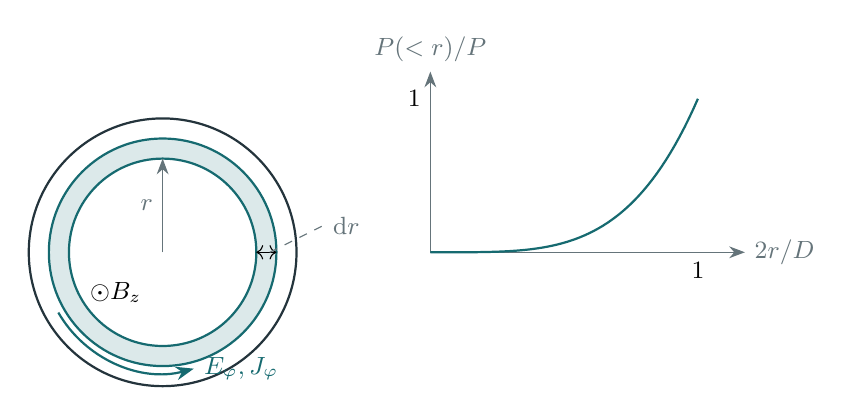
\begin{tikzpicture}[scale=.85]

\fill[accent!15,even odd rule] (0,0) circle(1.7) (0,0) circle(1.4);
\draw[object] (0,0) circle(2);\draw[traj] (0,0) circle(1.4);\draw[traj] (0,0) circle(1.7);
\draw[axis] (0,0)--(0,1.4) node[midway,left]{$r$};\draw[<->] (1.4,0)--(1.7,0);\draw[guide] (1.6,0)--(2.4,.4) node[right]{$\dd r$};
\node at(-.7,-.6){$\odot B_z$};\draw[motion] (210:1.8) arc(210:285:1.8) node[right]{$E_\varphi,J_\varphi$};
\draw[axis] (4,0)--(8.7,0) node[right]{$2r/D$};\draw[axis] (4,0)--(4,2.7) node[above]{$P(<r)/P$};
\draw[traj,domain=0:1,samples=60] plot ({4+4*\x},{2.3*\x^4});\node[below] at(8,0){$1$};\node[left] at(4,2.3){$1$};

\end{tikzpicture}\figcaption{解图电3.13A\quad 左图取$B_z>0,\dot B_z<0$，薄壳导电截面为$h\dd r$；右为径向累计功率占比。}\end{minipage}\end{center}

取解图电3.13A中的薄圆柱壳，半径$r$、厚$\dd r$、高$h$。沿周向导电的截面为$h\dd r$，电阻和回路电动势为
\[
\dd\mathcal R=\frac{2\pi r}{\sigma h\dd r},\qquad
\mathcal E_r=-\pi r^2\dot B_z.
\]
这里的 $\dd\mathcal R$ 表示厚度为 $\dd r$ 的一整圈导体的电阻。电流在每一半径处沿周向闭合，故沿半径累加各壳热功率：
\[
\dd P=\frac{\mathcal E_r^2}{\dd\mathcal R}
=\frac{\pi\sigma h}{2}r^3\dot B_z^{\,2}\dd r.
\]
由$r=0$积分到$D/2$，得到瞬时功率
\[
P(t)=\frac{\pi\sigma h}{2}\dot B_z^{\,2}\int_0^{D/2}r^3\dd r
=\frac{\pi\sigma hD^4}{128}\dot B_z^{\,2}.
\]
对一个周期平均，$\overline{\dot B_z^{\,2}}=\omega^2B_0^2/2=\omega^2B^2$，所以
\[
\boxed{\overline P=\frac{\pi\sigma hD^4\omega^2B^2}{128}
=\frac{\pi^3f^2\sigma B^2D^4h}{32}}.
\]
也可直接以$\sigma E_\varphi^2$乘薄壳体积$2\pi rh\dd r$，得到相同积分。解图电3.13A右侧给出半径$r$以内的功率占比$(2r/D)^4$，说明外层贡献较大。

均匀穿透近似要求圆柱半径远小于集肤深度$\delta=\sqrt{2/(\mu\sigma\omega)}$，并要求涡流产生的磁场不明显改变所给外场；柱体的有效加热区还需远离端部。随频率升高，集肤深度变小；当 $D/2$ 与 $\delta$ 同阶时，功率积分中的电场应换成实际径向分布。

把正弦磁场的变化率代回瞬时功率，得到
\[
P(t)=2\overline P\sin^2\omega t
=\overline P(1-\cos2\omega t).
\]
磁场取正、负极值时$\dot B_z=0$，涡流和瞬时热功率都为零；磁场过零而变化最快时发热最大。因此磁场每变化一个周期，热功率完成两次起伏，频率为 $2f$。沿半径积分又给
\[
\frac{P(<r)}{P(<D/2)}=\left(\frac{2r}{D}\right)^4.
\]
例如外侧一半半径范围贡献$1-(1/2)^4=15/16$的功率；若说的是外侧一半\emph{体积}，其内边界为$r=D/(2\sqrt2)$，贡献则为$3/4$。解图电3.13A右侧的横坐标是半径比，读图时应区分这两种“外层”定义。

\begin{center}\begin{minipage}{.97\linewidth}\centering
\begin{tikzpicture}[x=.8cm,y=1cm,font=\small]
\draw[axis](0,0)--(6.7,0)node[below right]{$\omega t$};\draw[axis](0,-1.3)--(0,1.5)node[above]{归一化量};
\draw[traj,domain=0:6.28318,samples=100,variable=\t]plot(\t,{cos(\t r)});
\draw[thick,warm,domain=0:6.28318,samples=100,variable=\t]plot(\t,{sin(\t r)^2});
\foreach\x/\lab in {1.5708/{\pi/2},3.14159/\pi,4.71239/{3\pi/2},6.28318/{2\pi}}{\node[below]at(\x,0){$\lab$};}
\node[right,accent]at(7,1){$B_z/B_0=\cos\omega t$};\node[right,warm]at(7,-.6){$P/P_{\max}=\sin^2\omega t$};
\end{tikzpicture}
\figcaption{解图电3.13B　磁场与瞬时热功率的相位。磁场极值处不发热，磁场过零处热功率最大，一周期出现两个峰。}
\end{minipage}\end{center}
\begin{center}\begin{minipage}{.97\linewidth}\centering
\begin{tikzpicture}[scale=.8,font=\small]
\foreach\x/\ri/\lab in {0/.8/{外半径一半},5/1.13137/{外体积一半}}{
\begin{scope}[xshift=\x cm]\fill[warm!25](0,0)circle(1.6);\fill[white](0,0)circle(\ri);\draw[object](0,0)circle(1.6);\draw[guide](0,0)circle(\ri);\node[above]at(0,2){\lab};\end{scope}}
\draw[axis](0,0)--(.8,0)node[midway,above]{$R/2$};\draw[axis](5,0)--(6.13137,0)node[midway,above]{$R/\sqrt2$};
\node[below]at(0,-1.9){外环功率$15\overline P/16$};\node[below]at(5,-1.9){外环功率$3\overline P/4$};
\end{tikzpicture}
\figcaption{解图电3.13C　同一圆柱的两种外层划分，$R=D/2$。半径范围和体积比例不同，两幅图的着色环从不同半径起算。}
\end{minipage}\end{center}

解图电3.13B中，周向场的相位由磁场求导得到。$\dot B_z=-\omega B_0\sin\omega t$，
所以$E_\varphi=(r\omega B_0/2)\sin\omega t$，在每个非零半径处与磁场相差四分之一周期。
周向电流每半周期反向，瞬时功率则始终非负。磁场从一个极值走向另一个极值时，周向电场方向保持，在两极值之间的过零时刻达到最大幅值。

解图电3.13C的两幅横截面显示金属体积与半径平方成正比，累计热功率却与半径四次方成正比。
设外层内边界为$\xi R$，外层体积比例为$1-\xi^2$，热功率比例为$1-\xi^4$。
给定外层体积比例p时，$\xi^2=1-p$，故外层热功率比例为$2p-p^2$。
给定同一个 $p$，先在解图电3.13C确定着色环的内缘，然后用解图电3.13A的累计功率曲线减去内圆所占比例。外层体积越薄，每单位体积的平均耗散越接近表面处的耗散密度。


\Needspace{13\baselineskip}

\pdfbookmark[2]{第 14 题 电压表引线路径与感生电压}{q14}

\section*{第 14 题\quad 电压表引线路径与感生电压}\label{q:14}

半径为$a$、总电阻为$r$的均匀圆形导线处于垂直圆面的匀强磁场中，磁感应强度以恒定速率$\dot B$变化。圆上两点$A,B$沿逆时针方向张角为$\theta$，$0<\theta<2\pi$。用内阻$R$的电压表连接两点，理想引线有两种接法：其一沿$A\to O\to B$两条半径连接，表头在圆心附近；其二沿直弦$AB$连接，表头位于弦上。忽略表头自身面积与自感，求两种读数，并解释理想电压表极限下的差别。

\begin{center}\begin{minipage}{.98\linewidth}\centering
\begin{tikzpicture}[scale=.85]

\foreach \shift in {0,6}{\begin{scope}[xshift=\shift cm]
\draw[object] (0,0) circle(1.8);\fill(0,0) circle(1pt) node[below]{$O$};
\fill(0:1.8) circle(1.4pt) node[right]{$A$};\fill(120:1.8) circle(1.4pt) node[above left]{$B$};
\draw (0:.6) arc(0:120:.6) node[midway,above]{$\theta$};\end{scope}}
\draw[traj] (1.8,0)--(0,0)--(120:1.8);\draw[fill=white] (0,0) circle(.22) node{$V$};
\draw[traj] (7.8,0)--(5.1,1.559);\draw[fill=white] (6.45,.779) circle(.22) node{$V$};
\node at(0,-2.3){径向引线};\node at(6,-2.3){沿弦引线};\node at(3,2.2){$\odot\ B(t)$};

\end{tikzpicture}\figcaption{图电3.14\quad 相同端点，两种实际测量路径。}\end{minipage}\end{center}

\Needspace{6\baselineskip}\subsection*{解答}

图电3.14中的两条圆弧电阻为
\[
r_1=\frac{r\theta}{2\pi},\qquad r_2=\frac{r(2\pi-\theta)}{2\pi}.
\]
先讨论径向引线。感生电场在径向没有分量，表头支路的感生电动势为零。两圆弧与两半径分别围成扇形，回路电动势的大小为
\[
e_1=\frac{a^2|\dot B|\theta}{2},\qquad
e_2=\frac{a^2|\dot B|(2\pi-\theta)}{2}.
\]
两弧电动势方向相反，但$e_1/r_1=e_2/r_2$。因此表头支路不分流，圆周上可维持连续环流，第一种读数为
\[
\boxed{V_{\text{径向}}=0}.
\]

\begin{center}\begin{minipage}{.98\linewidth}\centering
\begin{tikzpicture}[scale=.85]

\fill[warm!20] (0,0)--(1.8,0)--(120:1.8)--cycle;\draw[object] (0,0) circle(1.8);
\draw[traj] (1.8,0) node[right]{$A$}--(120:1.8) node[above left]{$B$};\draw[guide] (1.8,0)--(0,0)--(120:1.8);
\node[below] at(0,0){$O$};\node at(.45,.55){$S_\triangle$};
\draw[object] (4,0) rectangle (9,2.3);\node[fill=white] at(6.5,2.3){$R$（表头）};\node[fill=white] at(6.5,0){$r_1\parallel r_2$};
\draw[motion] (4.3,.4)--(4.3,1.9) node[midway,right]{$e_\triangle$};

\end{tikzpicture}\figcaption{解图电3.14A\quad 测量路径之间的三角形面积产生增量电动势；外圆两弧并联。}\end{minipage}\end{center}

解图电3.14A将引线从两半径改为弦。两条路径之间的三角形$OAB$有有向面积$a^2\sin\theta/2$，相应增加的有向感应电动势为
\[
e_\triangle=\frac12a^2\dot B\sin\theta
\]
（符号随所选回路方向改变，读数取绝对值）。在径向接法中已求得外圆两端的等效开路电势为零；改走弦相当于在测量支路加入这个路径电动势。外圆两弧的等效内阻为
\[
r_*=r_1\parallel r_2=\frac{r\theta(2\pi-\theta)}{4\pi^2}.
\]
表头电流与第二种读数为
\[
|I_V|=\frac{|e_\triangle|}{R+r_*},\qquad
\boxed{V_{\text{弦}}=\frac{R a^2|\dot B\sin\theta|}{2[R+r\theta(2\pi-\theta)/(4\pi^2)]}}.
\]
若$R\to\infty$，表头电流趋零，两种读数分别趋于$0$和$a^2|\dot B\sin\theta|/2$，仍可不同。电压表沿实际引线与内部支路响应电场作用，而随时间变化的磁场中总电场的线积分依赖路径。静电势差为端点量，沿弦和沿半径的实际测量各自包含相应的感生电场积分。

当$\theta=\pi$时，两半径合成同一直径，三角形有向面积为零，两种读数都为零，对应公式中的 $\sin\theta=0$。

把两条圆弧与测量路径接在同一对节点之间，可以直接由节点方程求有限内阻下的电势差。记$u=U_A-U_B$，取$\dot B>0$、$A\to B$逆时针弧张角$\theta$。两弧沿$A\to B$的有向电动势为
\[
e_a=-\frac{a^2\dot B\theta}{2},\quad
e_b=\frac{a^2\dot B(2\pi-\theta)}2,
\quad \frac{e_a}{r_1}+\frac{e_b}{r_2}=0.
\]
径向表支路的电动势为零，节点方程$ (u+e_a)/r_1+(u+e_b)/r_2+u/R=0$立即给$u=0$。弦支路的有向电动势为$-e_\triangle$，于是
\[
u\left(\frac1{r_1}+\frac1{r_2}+\frac1R\right)=\frac{e_\triangle}{R},\quad
u=\frac{r_*e_\triangle}{R+r_*},\quad
I_V=\frac{u-e_\triangle}{R}=-\frac{e_\triangle}{R+r_*}.
\]
取$R|I_V|$即回到读数公式。特别地，$R\to\infty$时静电势差$u\to0$，而$R|I_V|\to|e_\triangle|$，有限的表端电压来自路径感生项。解图电3.14A中的测量回路面积决定路径电动势，节点电荷再自行调整以满足电流守恒。

\begin{center}\begin{minipage}{.97\linewidth}\centering
\begin{tikzpicture}[scale=.8,font=\small]
\draw[object](0,0)--(0,2)--(6,2)--(6,-2)--(0,-2)--cycle;\draw[object](0,0)--(6,0);
\fill(0,0)circle(2pt)node[left]{$A$};\fill(6,0)circle(2pt)node[right]{$B$};
\foreach\y/\lab/\ii in {2/{r_1,e_a}/I_a,0/{r_2,e_b}/I_b,-2/{R,-e_\triangle}/I_V}{\node[fill=white]at(4,\y){$\lab$};\draw[motion](.7,\y)--(2,\y)node[midway,above]{$\ii$};}
\node[align=left]at(9.4,.5){全部取$A\to B$\\$I_a+I_b+I_V=0$\\$u=U_A-U_B$};
\end{tikzpicture}
\figcaption{解图电3.14B　弦接法的三支路网络，所有电流先按同一端点方向取正。不同路径的感生电动势按箭头带符号。}
\end{minipage}\end{center}

解图电3.14B对应的三支路电流为$I_a=(u+e_a)/r_1$、$I_b=(u+e_b)/r_2$、$I_V=(u-e_\triangle)/R$。
两弧的$e_a/r_1+e_b/r_2=0$使圆周自身不要求端点建立电势差，但弦支路的感生驱动破坏这一平衡。
从节点式保留每一项，令$G=1/r_1+1/r_2=1/r_*$，便有$u(G+1/R)=e_\triangle/R$。
这一步同时确定静电荷调整后的u和表头电流。当 $R$ 有限时，节点静电荷调整到 $u=r_*e_\triangle/(R+r_*)$。

分别沿两条弧与弦构成闭合回路。分别沿上弧去、弦返回及另一弧去、弦返回，把感生电动势相减，得到两回路的有向电动势$e_a+e_\triangle$与$e_b+e_\triangle$。
它们分别对应弓形区与剩余区的有向磁通，而两回路相减又恢复整圆磁通。
从径向接法转到弦接法时，两回路同时增添同一有向三角形面积。两条外圆弧各自的电动势保留原来的扇形值。
\begin{center}\begin{minipage}{.97\linewidth}\centering
\begin{tikzpicture}[x=2.5cm,y=2.5cm,font=\small]
\draw[axis](0,0)--(2.15,0)node[below right]{$\theta/\pi$};\draw[axis](0,0)--(0,1.2)node[above]{$V/(a^2|\dot B|/2)$};
\draw[traj,domain=0:2,samples=120,variable=\t]plot(\t,{abs(sin(180*\t))});
\draw[thick,warm,domain=0:2,samples=120,variable=\t]plot(\t,{abs(sin(180*\t))/(1+\t*(2-\t))});
\foreach\x/\lab in {.5/{1/2},1/1,1.5/{3/2},2/2}{\node[below]at(\x,0){$\lab$};}
\node[right,accent]at(2.3,1){$R\to\infty$};\node[right,warm]at(2.3,.6){$R=r/4$};\node[right]at(2.3,.2){径向接法恒为0};
\end{tikzpicture}
\figcaption{解图电3.14C　弦接法读数随节点位置变化的实际曲线。有限表内阻降低读数，但直径退化点与引线有向面积的零点不变。}
\end{minipage}\end{center}

解图电3.14C画的是读数的绝对值，所以在$\theta=\pi$处随有向电动势变号而出现零点。
取$R=r/4$，令$x=\theta/\pi$，归一化读数为$|\sin(\pi x)|/[1+x(2-x)]$；理想表曲线则为$|\sin(\pi x)|$。
两曲线都在直径处归零，有限表内阻仅改变幅度及极值位置；路径所围的有向面积依然由几何位置给出。


\Needspace{13\baselineskip}

\pdfbookmark[2]{第 15 题 增长磁场中圆形导轨上的带电珠}{q15}

\section*{第 15 题\quad 增长磁场中圆形导轨上的带电珠}\label{q:15}

质量$m$、正电荷量$q$的小珠可在半径$R$的绝缘光滑水平圆形导轨上运动。垂直导轨平面向外的匀强磁场，在$0<t<T$内从零均匀增加到$B_0$，随后保持不变；磁场关于导轨圆心轴对称。小珠起初静止，不计辐射和电磁反作用。求小珠的速率、位移角，以及它对导轨的水平作用力随时间的变化。

\begin{center}\begin{minipage}{.98\linewidth}\centering
\begin{tikzpicture}[scale=.85]

\draw[object] (0,0) circle(1.8);\fill(0,0) circle(1.2pt) node[below]{$O$};
\draw[axis] (0,0)--(1.8,0) node[midway,above]{$R$};\fill[accent] (1.8,0) circle(3pt) node[right]{$m,q$};
\node at(-.5,.7){$\odot B(t)$};\node at(5.5,1){$0\to B_0$，历时$T$};\node at(5.5,0){随后$B=B_0$};

\end{tikzpicture}\figcaption{图电3.15\quad 初始珠子静止；磁场增长在圆周上激发感生电场。}\end{minipage}\end{center}

\Needspace{6\baselineskip}\subsection*{解答}

以从上方观察的顺时针角位移$\theta$为正。磁场向外增加，感生电场沿顺时针，圆周上大小为
\[
E_\varphi=\frac{R}{2}\frac{B_0}{T}.
\]
电场力沿切线加速小珠，磁场力和导轨的水平力均沿半径，因此切向方程只含电场力。由$m\dot v=qE_\varphi$及初始静止，得到
\[
v(t)=\begin{cases}\dfrac{qB_0R}{2mT}t,&0\le t\le T,\\[2pt]\dfrac{qB_0R}{2m},&t\ge T,\end{cases}
\]
\[
\theta(t)=\begin{cases}\dfrac{qB_0}{4mT}t^2,&0\le t\le T,\\[2pt]\dfrac{qB_0T}{4m}+\dfrac{qB_0}{2m}(t-T),&t\ge T.\end{cases}
\]

\begin{center}\begin{minipage}{.98\linewidth}\centering
\begin{tikzpicture}[scale=.85]

\draw[guide] (0,0) circle(1.7);\fill(0,0) circle(1pt) node[below]{$O$};\fill[accent](1.7,0) circle(3pt);
\draw[force] (1.7,.12)--(.4,.12) node[midway,above]{$qvB$};\draw[force](1.7,0)--(3.1,0) node[right]{$N'$};
\draw[force](1.7,-.1)--(1.7,-1.4) node[left]{$qE$};\draw[motion](2.4,-.1)--(2.4,-1.4) node[right]{$v$};
\node at(-.5,.7){$\odot B$};\node at(.4,2.3){$0<t<T$};
\draw[axis](5,0)--(10,0) node[right]{$t/T$};\draw[axis](5,0)--(5,2.7) node[above]{$N/N(T)$};
\draw[traj,domain=0:1] plot ({5+2.5*\x},{2*(\x)^2});\draw[traj](7.5,2)--(9.5,2);
\draw[guide](7.5,0)--(7.5,2);\node[below] at(7.5,0){$1$};

\end{tikzpicture}\figcaption{解图电3.15A\quad 左图为磁场增长阶段的珠子受力与速度，$N'$向外；右图为珠子对轨道的力大小。}\end{minipage}\end{center}

解图电3.15A在小珠所在位置将切向与径向受力分开。顺时针速度与向外磁场形成向心洛伦兹力。对$0<t<T$，
\[
F_B=qvB(t)=\frac{q^2B_0^2R}{2mT^2}t^2,
\qquad
\frac{mv^2}{R}=\frac{q^2B_0^2R}{4mT^2}t^2=\frac12F_B.
\]
磁力比所需向心力大，故导轨对珠子的水平力 $N^\prime$ 向外，抵去部分向心磁力。取径向向内为正，有$F_B-N'=mv^2/R$，所以
\[
N'=\frac{q^2B_0^2R}{4mT^2}t^2.
\]
小珠对导轨的水平作用力与$N'$相反，指向圆心，大小为
\[
\boxed{N(t)=\begin{cases}\dfrac{q^2B_0^2R}{4mT^2}t^2,&0\le t\le T,\\[2pt]\dfrac{q^2B_0^2R}{4m},&t\ge T.\end{cases}}
\]
在$t=T$处速率和水平作用力连续，切向加速度则因$\dot B$变为零而改变。此后$E_\varphi=0$，小珠保持匀速圆周运动，磁力与导轨力继续提供合向心力。

对切向电场力沿位移做功积分，得 $\Delta K=\int_0^T qE_\varphi v\dd t=q^2B_0^2R^2/(8m)$。在增长阶段，电场力提供动能，两个径向力与速度垂直。竖直方向的重力与支持力互相平衡，不属于题目所求水平作用力。

还可由切向角动量直接积分，解释终速度与增长时间无关。取逆时针有向切向速度$v_\varphi$，有
\[
\frac{\dd(mRv_\varphi)}{\dd t}=qRE_\varphi
=-\frac{qR^2}{2}\dot B,
\qquad
mRv_\varphi+\frac{qR^2B}{2}=0.
\]
所以$v_\varphi=-qRB/(2m)$，对正电荷及向外增长的$B$即为顺时针运动。电场力矩使机械角动量 $mRv_\varphi$ 随向外磁场增强而变得更负，增加的是顺时针角动量的大小。与之相加的磁场项随 $B$ 增大。

解图电3.15A左图只表示$0<t<T$的增长阶段，$qE$与速度$v$分别标注；$t>T$时应擦去$qE$箭头而保留速度和两径向力。最终磁力$qvB_0$恰为所需向心力的两倍，轨道反力向外抵消其中一半；这些径向力均不做功，故终动能完全由切向电场功提供。

\begin{center}\begin{minipage}{.97\linewidth}\centering
\begin{tikzpicture}[scale=.8,font=\small]
\draw[guide](0,0)circle(1.6);\fill(0,0)circle(1pt)node[below]{$O$};\fill[accent](1.6,0)circle(3pt);
\draw[force](1.6,.15)--(-.3,.15)node[midway,above]{$qvB_0$};
\draw[force](1.6,-.15)--(2.7,-.15)node[right]{$N'$};\draw[motion](3.5,.7)--(3.5,-.6)node[right]{$v_T$};
\node[above]at(.3,2){珠子受力，$t>T$};\node at(-.4,.8){$\odot B_0$};
\draw[guide](7,0)circle(1.6);\fill[warm](8.6,0)circle(3pt);\draw[force](8.6,0)--(7.4,0)node[midway,above]{$N$};
\node[above]at(7,2){珠子对环的作用力};\node[below]at(7,-1.9){$N=N'$，方向相反};
\end{tikzpicture}
\figcaption{解图电3.15B　恒定磁场阶段及作用反作用。左图只画珠子受力，右图只画珠子对环的力；切向电场已消失。}
\end{minipage}\end{center}
\begin{center}\begin{minipage}{.97\linewidth}\centering
\begin{tikzpicture}[x=2.6cm,y=2.6cm,font=\small]
\draw[axis](0,0)--(2.2,0)node[below right]{$t/T$};\draw[axis](0,0)--(0,1.2)node[above]{归一化量};
\draw[traj](0,0)--(1,1)--(2,1);\draw[thick,warm,domain=0:1,samples=60,variable=\t]plot(\t,{\t^2});\draw[thick,warm](1,1)--(2,1);
\draw[guide](1,0)--(1,1);\node[below]at(1,0){$1$};\node[left]at(0,1){$1$};
\node[right,accent]at(2.35,.8){$v/v_T$：直线后平台};\node[right,warm]at(2.35,.4){$N/N_T$：抛物线后平台};
\end{tikzpicture}
\figcaption{解图电3.15C　速率与作用力的真实时间曲线，$v_T=qB_0R/(2m)$、$N_T=q^2B_0^2R/(4m)$。两者在$t=T$连续，增长阶段的幂次不同。}
\end{minipage}\end{center}

在解图电3.15B左侧，研究对象是恒场阶段的小珠。速度仍顺时针，洛伦兹力指向O，大小$qv_TB_0$；轨道力沿半径向外，大小$N'$。
它们的合力应等于$mv_T^2/R$，所以$N'=qv_TB_0-mv_T^2/R$。
代$v_T=qB_0R/(2m)$后，两项分别为$q^2B_0^2R/(2m)$和$q^2B_0^2R/(4m)$，得到正的外向轨道力。
右侧以导轨为受力物体，画小珠对导轨的作用力 $N$，从接触点指向圆心 $O$。

小珠的重力和竖直支持力平衡。绝缘导轨作为机械约束，限制小珠的径向位置；感生电场则沿轨道切线作用于电荷。由切向冲量确定 $v$ 之后，将 $qvB$ 与半径为 $R$ 的向心需求 $mv^2/R$ 相减，得到导轨反力。

解图电3.15C显示增长阶段如何过渡到恒场阶段。$t=T$两侧B和v都连续，故磁力、向心需求以及N均连续；改变的是$\dot B$，所以电场力和切向加速度从常量跃变为零。
图中速度斜率由正值变零，但没有速度跳变；N曲线由二次增长接恒值，也没有冲量。
恒场阶段，径向合力使速度方向连续沿圆周转动，速率保持为 $v_T$。

位移角应另做一次时间积分。增长阶段平均速率为$v_T/2$，故$\theta(T)=v_TT/(2R)$；恒场阶段再加$v_T(t-T)/R$，与前面的分段式一致。
延长增长时间会改变这一角位移，但终速和终轨道作用力由磁场总变化决定。转动持续的时间与终端动力学条件分别进入两类结果，因而角位移在增长段为时间的二次函数，进入恒场后改为一次函数。


\Needspace{13\baselineskip}

\pdfbookmark[2]{第 16 题 螺线管断电时带电圆盘的转动}{q16}

\section*{第 16 题\quad 螺线管断电时带电圆盘的转动}\label{q:16}

半径$r$、质量$m$的均匀绝缘圆盘可绕中心轴无摩擦转动，轮缘均匀固定$N$个电荷量均为$q>0$的小珠，小珠质量忽略。半径$a<r$、单位长度$n$匝的长螺线管与圆盘同轴，初始电流为$I$且圆盘静止；随后电流降至零。忽略端部磁场、辐射和圆盘电荷对磁场的影响，求最终角速度及方向，并说明它是否取决于断电快慢。

\begin{center}\begin{minipage}{.98\linewidth}\centering
\begin{tikzpicture}[scale=.85]

\fill[accent!10] (0,0) circle(1.1);\draw[object] (0,0) circle(2);\draw[traj] (0,0) circle(1.1);
\foreach \ang in {0,45,90,135,180,225,270,315}{\fill[warm] (\ang:2) circle(2.5pt);}
\draw[axis] (0,0)--(0,1.1) node[midway,left]{$a$};\draw[axis] (0,0)--(2,0) node[midway,below]{$r$};
\node at(-.5,-.4){$\odot B$};\node[align=left] at(5,1){内圆：螺线管场区\\外圆：圆盘边缘\\轮缘共$N$个电荷$q$};

\end{tikzpicture}\figcaption{图电3.16\quad 轮缘在磁场区域外；电流从$I$降至零。}\end{minipage}\end{center}

\Needspace{6\baselineskip}\subsection*{解答}

图电3.16中，磁场只在螺线管内部近似均匀，$B(t)=\mu_0ni(t)$，圆盘轮缘位于场区外。取初始磁场向外，逆时针为正。半径$r$的积分圆所包围的磁通来自半径$a$的区域：
\[
2\pi r E_\varphi=-\pi a^2\mu_0n\dot i,
\qquad
E_\varphi=-\frac{\mu_0na^2}{2r}\dot i.
\]
左式沿半径 $r$ 的圆周积分，右式仅取半径 $a$ 内磁场随时间的变化。

\begin{center}\begin{minipage}{.98\linewidth}\centering
\begin{tikzpicture}[scale=.85]

\fill[accent!12] (0,0) circle(1.1);\draw[traj] (0,0) circle(1.1);\draw[guide] (0,0) circle(2);
\fill[warm] (2,0) circle(3pt) node[right]{$q$};\draw[force] (2,0)--(2,1.3) node[right]{$qE_\varphi$};
\draw[axis] (0,0)--(2,0) node[midway,below]{$r$};\node at(0,.4){$\pi a^2$};\node at(0,-.5){$\odot B\downarrow$};
\draw[motion] (30:2.2) arc(30:105:2.2) node[above]{$\omega>0$};
\node[align=left] at(5.9,1){$2\pi rE_\varphi=-\pi a^2\dot B$\\$\tau=NrqE_\varphi$\\$\Delta(J\omega)=\frac12\mu_0nNqa^2I$};

\end{tikzpicture}\figcaption{解图电3.16A\quad 积分圆周长用$r$，链接磁通面积用$a$；电场力提供角冲量。}\end{minipage}\end{center}

解图电3.16A将一个小珠的切向电场力与力臂$r$画出。$N$个电荷对轴的总力矩为
\[
\tau=NrqE_\varphi=-\frac12\mu_0nNqa^2\dot i.
\]
圆盘转动惯量为$J=mr^2/2$。对从$i=I$到$i=0$的全过程积分角动量方程：
\[
J\omega=\int\tau\dd t
=-\frac12\mu_0nNqa^2\int_I^0\dd i
=\frac12\mu_0nNqa^2I.
\]
故
\[
\boxed{\omega=\frac{\mu_0nNqIa^2}{mr^2}}.
\]
正号对应逆时针，即正电荷运动产生的磁场试图维持初始向外磁通。断电较快时感生电场较强、作用时间较短；较慢时相反，二者的角冲量只由电流的总变化决定，因此终角速度与断电的具体时间规律无关。

圆盘所得转动能为$J\omega^2/2$，由感生电场做功提供。按题设给定的螺线管电流演化，盘只受已算出的感生电场力矩。若小珠每个质量为$m_b$，只需把$J$改为$mr^2/2+Nm_br^2$，角冲量式仍成立。

对任意中间时刻积分同一个力矩方程，可得
\[
J\omega(t)=C[I-i(t)],\qquad
C=\frac12\mu_0nNqa^2.
\]
因此电流减小多少，圆盘获得的角动量就增加多少。若电流在$0<t<T$线性减至零，$\omega(t)=\omega_f t/T$，断电期间的角位移为$\omega_fT/2$；其他断电规律虽给相同$\omega_f$，角位移可不同。

由感生力矩求机械功：$P=\tau\omega=J\omega\dot\omega$，故$W=\int_0^{\omega_f}J\omega\dd\omega=J\omega_f^2/2$。解图电3.16A中用$a$决定场区磁通、用$r$决定力臂与惯量，最终$\omega_f\propto a^2/r^2$，场外的感生电场仍在轮缘电荷上做功。

\begin{center}\begin{minipage}{.97\linewidth}\centering
\begin{tikzpicture}[x=4.5cm,y=2.6cm,font=\small]
\draw[axis](0,0)--(1.1,0)node[below right]{$t/T$};\draw[axis](0,0)--(0,1.2)node[above]{$\omega/\omega_f$};
\draw[traj](0,0)--(1,1);\draw[thick,warm,domain=0:1,samples=60,variable=\t]plot(\t,{\t^2});
\node[below]at(1,0){$1$};\node[left]at(0,1){$1$};\draw[guide](1,0)--(1,1);
\node[right,accent]at(1.2,.9){$i/I=1-t/T$};\node[right,warm]at(1.2,.4){$i/I=1-(t/T)^2$};
\end{tikzpicture}
\figcaption{解图电3.16B　两种完全断电过程的角速度。相同终值对应不同曲线面积，所以角位移不同。}
\end{minipage}\end{center}

解图电3.16B先指定电流规律，再由同一中间态公式求角速度。取 $i=I(1-t/T)$ 得 $\omega=\omega_f t/T$，取 $i=I[1-(t/T)^2]$ 得 $\omega=\omega_f(t/T)^2$。
对两条角速度曲线分别积分，角位移为$\omega_fT/2$和$\omega_fT/3$。它们的末角速度相同，说明所受总角冲量相同。二次历程的电场峰值在末端，大小为线性历程的两倍。
这里角冲量应看力矩曲线的面积，角位移应看角速度曲线的面积，二者的纵轴不同。
\begin{center}\begin{minipage}{.97\linewidth}\centering
\begin{tikzpicture}[x=1.7cm,y=2.6cm,font=\small]
\draw[axis](0,0)--(3.4,0)node[below right]{$\rho/a$};\draw[axis](0,0)--(0,1.25)node[above]{$E_\varphi/E_a$};
\draw[traj](0,0)--(1,1);\draw[traj,domain=1:3.2,samples=70,variable=\t]plot(\t,{1/\t});
\draw[guide](1,0)--(1,1);\node[below]at(1,0){$1$};\node[left]at(0,1){$1$};
\node[right]at(3.5,.9){场内$E_\varphi\propto\rho$};\node[right]at(3.5,.45){场外$E_\varphi\propto1/\rho$};
\end{tikzpicture}
\figcaption{解图电3.16C　同一时刻的完整径向感生场，$E_a=-a\dot B/2$。场外的局部磁场近于零，但感生电场随距离连续衰减。}
\end{minipage}\end{center}

解图电3.16C将A图的两种半径推广到任意积分半径$\rho$。圆周内实际磁通为$\pi\rho^2B$（$\rho<a$）或$\pi a^2B$（$\rho>a$），故
\[
E_\varphi(\rho)=-\frac{\dot B}{2}
\begin{cases}\rho,&0\le\rho\le a,\\a^2/\rho,&\rho\ge a.\end{cases}
\]
两段在$\rho=a$连续。轮缘$r>a$处应选下降的场外分支；将它乘力臂r后，单珠力矩中r抵消，但盘的转动惯量仍含$r^2$。
盘的力矩由场区内磁通的变化确定。盘半径改变时，在轮缘都位于场外且盘质量固定的条件下，终角速度随转动惯量的倒数变化。


\Needspace{13\baselineskip}

\pdfbookmark[2]{第 17 题 偏心感生电场驱动细管中的简谐运动}{q17}

\section*{第 17 题\quad 偏心感生电场驱动细管中的简谐运动}\label{q:17}

半长为$R$的绝缘光滑水平细管$MN$沿$x$轴放置，中点为$O$，$M,N$坐标分别为$-R,+R$。轴对称磁场的轴穿过$O'=(0,-d)$，在管道所在平面内磁场均匀且$B_z=-B_0\sin\omega t$，$B_0>0$。令$\angle MO'O=\theta_0$，故$d=R/\tan\theta_0$。质量$m$、正电荷量$q$的小珠在$t=0$由$N$处静止释放。取何种$\omega$可使小珠恰在$M,N$间以$O$为中心做简谐运动？求小珠对管的横向水平作用力$N_y(x)$，正方向取$+y$。忽略珠子的电磁反作用。

\begin{center}\begin{minipage}{.98\linewidth}\centering
\begin{tikzpicture}[scale=.85]

\draw[object] (-3,0) node[left]{$M(-R)$}--(3,0) node[right]{$N(R)$};\fill(0,0) circle(1pt) node[above]{$O$};
\fill(0,-2) circle(1.5pt) node[below]{$O'$};\draw[guide] (-3,0)--(0,-2)--(3,0) (0,-2)--(0,0);
\draw (0,-1.4) arc(90:146.3:.6) node[midway,left]{$\theta_0$};\node[right] at(0,-1){$d$};
\fill[accent] (3,0) circle(3pt);\node at(3,1){初始$m,q$静止};\node at(-3.5,-1.8){$B_z=-B_0\sin\omega t$};
\draw[axis] (1.1,.5)--(2,.5) node[right]{$x$};\draw[axis] (1.1,.5)--(1.1,1.4) node[above]{$y$};

\end{tikzpicture}\figcaption{图电3.17\quad 管中心与感生电场轴心相距$d$，不应混作同一点。}\end{minipage}\end{center}

\Needspace{6\baselineskip}\subsection*{解答}

轴对称感生电场绕$O'$，由法拉第定律，在相对$O'$的位置$(x,d)$处有
\[
\vect E=\frac{B_0\omega\cos\omega t}{2}(-d\,\vect e_x+x\,\vect e_y).
\]
图电3.17中沿管的分量$E_x$与$x$无关。沿管电场在整条管内同相变化。对这个时间驱动积分，再用珠子的初始位置及速度，才能确定振动中心。

\begin{center}\begin{minipage}{.98\linewidth}\centering
\begin{tikzpicture}[scale=.85]

\draw[object] (-2.5,0)--(3.2,0);\fill(0,0) circle(1pt) node[above]{$O$};\fill(0,-2) circle(1pt) node[below]{$O'$};
\fill[accent] (1.8,0) circle(3pt) node[above right]{$x$};\draw[guide] (0,-2)--(1.8,0);
\draw[force] (1.8,0)--(.5,0) node[midway,above]{$qE_x$};\draw[force] (1.8,0)--(1.8,1.2) node[above]{$qE_y$};
\draw[force] (2.1,-.1)--(2.1,-1.4) node[right]{$F_{By}$};
\node[align=left] at(6,0){所示时刻：$0<\omega t<\pi/2$\\$E_x=-dB_0\omega\cos\omega t/2$\\$E_y=xB_0\omega\cos\omega t/2$};

\end{tikzpicture}\figcaption{解图电3.17A\quad 管上感生电场的两个分量与洛伦兹磁力；示图取第一四分之一周期。}\end{minipage}\end{center}

解图电3.17A中，磁力垂直于速度，不含$x$分量。因此
\[
m\ddot x=-\frac{qB_0\omega d}{2}\cos\omega t.
\]
使用$x(0)=R,\dot x(0)=0$两次积分：
\[
\dot x=-\frac{qB_0d}{2m}\sin\omega t,\qquad
x=R-A+A\cos\omega t,\quad A=\frac{qB_0d}{2m\omega}.
\]
振动中心为$R-A$、振幅为$A$。要使中心为$O$且端点为$\pm R$，须$A=R$，故
\[
\boxed{\omega=\frac{qB_0}{2m\tan\theta_0}},\qquad
x=R\cos\omega t,\quad v_x=-R\omega\sin\omega t.
\]
横向电场力为$qE_y=qB_0\omega x\cos\omega t/2=qB_0\omega x^2/(2R)$。磁力的$y$分量应从叉乘求符号：
\[
F_{By}=-qv_xB_z=-qB_0\omega R\sin^2\omega t
=-\frac{qB_0\omega}{R}(R^2-x^2).
\]
管使珠子始终留在$y=0$，故管对珠子的力抵消上述两力；取反得到珠子对管的力，与两个电磁力的横向和同向：
\[
\boxed{N_y=qE_y+F_{By}
=\frac{qB_0\omega}{2R}(3x^2-2R^2)
=\frac{q^2B_0^2}{4mR\tan\theta_0}(3x^2-2R^2)}.
\]

\begin{center}\begin{minipage}{.98\linewidth}\centering
\begin{tikzpicture}[scale=.85]

\draw[axis] (-3,0)--(3.6,0) node[right]{$x/R$};\draw[axis] (0,-2.3)--(0,1.8) node[above]{$N_y/(qB_0\omega R)$};
\draw[traj,domain=-1:1,samples=60] plot ({2.5*\x},{2*(1.5*(\x)^2-1)});
\node[below] at(-2.5,0){$-1$};\node[below] at(2.5,0){$1$};\node[right] at(0,-2){$-1$};\node[right] at(0,1){$1/2$};
\draw[guide] (-2.5,0)--(-2.5,1) (2.5,0)--(2.5,1);\fill(-2.041,0) circle(1.6pt);\fill(2.041,0) circle(1.6pt);
\node[align=left] at(7.6,-.6){两个零点：$x=\pm R\sqrt{2/3}$\\中心：磁力作用为主\\端点：磁力为零};

\end{tikzpicture}\figcaption{解图电3.17B\quad 珠子对管的有向水平作用力；负值表示沿$-y$。}\end{minipage}\end{center}

解图电3.17B的抛物线在$x=0$取最小值$-qB_0\omega R$，在$x=\pm R\sqrt{2/3}$变号，在两端取$qB_0\omega R/2$。珠子在中心速度最大且电场横向分量为零，作用力由向$-y$的磁力决定；在两端速度为零，横向作用由电场力决定。端点与管中点因此分别对应图B的最大值和最小值。

代入选定频率后，可计算沿管力与动能的关系。沿实际轨迹$\cos\omega t=x/R$，沿管电场力成为$F_x=-m\omega^2x$，所以
\[
\frac12mv_x^2=\frac12m\omega^2(R^2-x^2),\qquad
\dd K=F_x\dd x.
\]
这是特定初值轨迹上的关系；外场本身仍是按时间给定的驱动。磁力不做功，管的约束力沿$y$而位移沿$x$，也不做功。小珠由$N$走到$M$再返回，一周期内电场的净功为零，横向作用力的平均另由其时间分布确定。

若频率没有选到题给值，一般轨迹的中心是$R-A$，范围为$[R-2A,R]$。当$A>R$时还可能碰到管的左端，余下运动取决于碰撞过程。以 $O$ 为中心且覆盖整管的条件为 $A=R$。

\begin{center}\begin{minipage}{.97\linewidth}\centering
\begin{tikzpicture}[scale=.8,font=\small]
\foreach\dx/\xv/\tl in {0/R/0,4/0/{\pi/2},8/{-R}/\pi}{\begin{scope}[xshift=\dx cm]
\draw[object](-1.4,0)--(1.4,0);\fill[accent](0,0)circle(3pt);\node[above]at(0,1.8){$\omega t=\tl,\ x=\xv$};\end{scope}}
\draw[force](0,0)--(0,.6)node[right]{$qE_y$};\node[below]at(0,-1.5){$N_y=F_0/2$};
\draw[force](4,0)--(4,-1.2)node[right]{$F_{By}$};\node[below]at(4,-1.5){$N_y=-F_0$};
\draw[force](8,0)--(8,.6)node[right]{$qE_y$};\node[below]at(8,-1.5){$N_y=F_0/2$};
\end{tikzpicture}
\figcaption{解图电3.17C　三个位形中作用于珠子的电磁横向合力，$F_0=qB_0\omega R$。珠子对管的$N_y$与该合力同向；管对珠子的约束力相反。}
\end{minipage}\end{center}

解图电3.17C的两端横向电场力都向上，电场方向由位置与时间相位的乘积决定。
在$t=0$时$x=R,\cos\omega t=1$；在$t=\pi/\omega$时$x=-R,\cos\omega t=-1$，两者的$x\cos\omega t$都为正。
中心处$x=0$使$E_y=0$，此时速度和磁场各为非零极值，洛伦兹力向下，故中间一帧的横向作用反向。
这三帧分别给B图抛物线两端和顶点的物理依据，零点则出现在电场横向力与磁力恰好抵消处。

把实际轨迹代入横向作用，写出随时间变化的力：
\[
N_y(t)=\frac{F_0}{2}(3\cos^2\omega t-2)
=\frac{F_0}{4}(3\cos2\omega t-1).
\]
珠子运动频率为$\omega$，管的横向受力却含常量和$2\omega$分量。
往返相同位置时电场相位与x的关系相同，磁力中$v_xB_z$也只含$\sin^2\omega t$，所以本题才可将$N_y$写成单值的$N_y(x)$。
含初速漂移时，位置与驱动相位的关系随时间改变，横向力要从电场和磁场的时间式计算。


\Needspace{13\baselineskip}

\pdfbookmark[2]{第 18 题 无电阻线框穿越窄磁场带的分段运动}{q18}

\section*{第 18 题\quad 无电阻线框穿越窄磁场带的分段运动}\label{q:18}

质量$m=0.10\,\mathrm{kg}$、边长$\ell=0.80\,\mathrm m$的正方形无电阻线框，自感$L=1.0\times10^{-3}\,\mathrm H$，在光滑水平面向右运动。匀强磁场垂直纸面向里，$B=0.50\,\mathrm T$，仅在$0<x<s$的长条区域存在，$s=0.20\,\mathrm m$。$t=0$时线框右边$bc$恰在$x=0$、左边$ad$在$x=-\ell$，初始电流为零。分别取初速度$v_0=4.0\,\mathrm{m/s}$和$v_0=16/\sqrt3\,\mathrm{m/s}$，求$t_0=\pi/36\,\mathrm s$时右边$bc$的位置$x$。忽略辐射与接触问题，自感保持不变。

\begin{center}\begin{minipage}{.98\linewidth}\centering
\begin{tikzpicture}[scale=.73]

\fill[accent!10](0,-.4) rectangle(1,4.4);\draw[guide](0,-.4)--(0,4.4) (1,-.4)--(1,4.4);
\draw[object](-4,0) node[below]{$d$}--(0,0) node[below left]{$c$}--(0,4) node[above left]{$b$}--(-4,4) node[above]{$a$}--cycle;
\draw[motion](-1,4.6)--(.5,4.6) node[right]{$v_0$};\node at(.5,2){$\otimes B$};
\draw[axis](-4.5,-.8)--(4,-.8) node[right]{$x$};\node[below] at(0,-.8){$0$};\node[below] at(1,-.8){$s$};\node[below] at(-4,-.8){$-\ell$};
\draw[<->](-4.6,0)--(-4.6,4) node[midway,left]{$\ell$};

\end{tikzpicture}\figcaption{图电3.18\quad 正方形框的边长为$\ell=4s$，初始右边$bc$在场区入口。}\end{minipage}\end{center}

\Needspace{6\baselineskip}\subsection*{解答}

线框电阻为零，外磁通的变化由自感电动势补偿。取线框逆时针电流为正，法线向外；当右边处于磁场带内而左边仍在外时，外磁通为$\Phi_e=-B\ell x$。由$L\dot I=-\dot\Phi_e$及初值可得磁链守恒：
\[
LI+\Phi_e=0,\qquad I=\frac{B\ell x}{L}.
\]
该阶段右边受向左安培力，故
\[
m\ddot x=-B\ell I=-\frac{B^2\ell^2}{L}x,
\quad \Omega=\frac{B\ell}{\sqrt{mL}}=40\,\mathrm{s^{-1}}.
\]
初始$x=0,\dot x=v_0$，所以$x=(v_0/\Omega)\sin\Omega t$。这段正弦运动对应右边在场带内、左边处在入口外的几何。

\begin{center}\begin{minipage}{.98\linewidth}\centering
\begin{tikzpicture}[scale=.70]

\foreach \shift in {0,7}{\begin{scope}[xshift=\shift cm]
\fill[accent!10](0,-.4) rectangle(1,4.4);\draw[guide](0,-.4)--(0,4.4) (1,-.4)--(1,4.4);
\node[below] at(0,-.4){$0$};\node[below] at(1,-.4){$s$};\end{scope}}
\draw[object](-3.5,0) rectangle(.5,4);\draw[force](.5,2)--(-.6,2) node[above]{$F_x<0$};\node[below] at(.5,0){$x$};
\draw[object](5.5,0) rectangle(9.5,4);\node[above] at(9.5,4){$x$};\draw[motion](9.5,.7)--(9.5,2.2) node[right]{$I$};
\node at(-1.5,4.9){进入：$\Phi_e=-B\ell x$};\node at(7.5,4.9){平台：$\Phi_e=-B\ell s$};
\node at(-1.5,-1.2){$I=B\ell x/L$，有回复力};\node at(7.5,-1.2){$I=B\ell s/L$，合力为零};

\end{tikzpicture}\figcaption{解图电3.18A\quad 两阶段线框均为正方形；平台阶段两竖边在场外，上下边所受的横向磁力相消。}\end{minipage}\end{center}

\textbf{第一种初速度。} 对照解图电3.18A中线框两竖边相对于磁场边界的位置，振幅$v_0/\Omega=0.10\,\mathrm m<s$，线框右边达不到磁场带的右边界，先减速停止再向左返回。到$t_1=\pi/\Omega=\pi/40\,\mathrm s$时，右边回到$x=0$，电流也降为零，速度为$-v_0$。随后整个线框在磁场左侧，不再有外磁通或安培力，因而匀速向左。由于$t_0>t_1$，
\[
\boxed{x(t_0)=-4\left(\frac\pi{36}-\frac\pi{40}\right)
=-\frac\pi{90}\,\mathrm m\simeq-0.03491\,\mathrm m}.
\]
回程至 $x=0$ 后，改用以该时刻和速度为初值的匀速式。

\textbf{第二种初速度。} 此时$v_0/\Omega=2/(5\sqrt3)\,\mathrm m>s$，右边能够越过磁场带。第一次到$x=s$时，
\[
\sin\Omega t_2=\frac{s\Omega}{v_0}=\frac{\sqrt3}{2},\quad
t_2=\frac\pi{120}\,\mathrm s,\quad
v_2=v_0\cos\frac\pi3=\frac8{\sqrt3}\,\mathrm{m/s}.
\]
在$s<x<\ell$时，磁场带全部位于框内，两竖边都不在场区；外磁通固定为$-B\ell s$，电流保持$B\ell s/L$。此时合磁力为零，线框以 $v_2$ 匀速前进。

\begin{center}\begin{minipage}{.97\linewidth}\centering
\begin{tikzpicture}[x=.8cm,y=.8cm,font=\small]
\draw[axis](0,0)--(4.4,0)node[below right]{$\Omega t$};\draw[axis](0,-1.15)--(0,1.5)node[above]{$x/A$};
\draw[traj,domain=0:3.14159,samples=80,variable=\t]plot(\t,{sin(\t r)});\draw[traj](3.14159,0)--(4.2,{-(4.2-pi)});
\draw[guide](3.14159,-1.1)--(3.14159,1.1);\node[above right]at(3.14159,0){$\pi$};
\fill({10*pi/9},{-pi/9})circle(2pt);\node[below left]at({10*pi/9},{-pi/9}){$t_0$};\node[above]at(2,2.5){$v_0=4,\ A=0.10\,\mathrm m$};
\begin{scope}[xshift=7cm]
\draw[axis](0,0)--(4.4,0)node[below right]{$\Omega t$};\draw[axis](0,0)--(0,3.3)node[above]{$x/s$};
\draw[traj,domain=0:1.047198,samples=50,variable=\t]plot(\t,{2/sqrt(3)*sin(\t r)});
\draw[traj](1.047198,1)--(4.2,{1+(4.2-pi/3)/sqrt(3)});
\draw[guide](0,1)--(4.2,1);\node[left]at(0,1){$1$};\node[below]at(1.047198,0){$\pi/3$};
\fill({10*pi/9},{1+7*pi/(9*sqrt(3))})circle(2pt);\node[right]at({10*pi/9},{1+7*pi/(9*sqrt(3))}){$t_0$};
\node[above]at(2,3.8){$v_0=16/\sqrt3$};\end{scope}
\end{tikzpicture}
\figcaption{解图电3.18B　按实际分段函数画出两种位置曲线，横轴均为$\Omega t$，纵轴各自归一化。切换处位置与斜率连续，实点标$t_0=\pi/36\,\mathrm s$。}
\end{minipage}\end{center}


解图电3.18B将两个速度对应的事件时间标开。代入$t_0$得到
\[
\boxed{x(t_0)=s+\frac8{\sqrt3}\left(\frac\pi{36}-\frac\pi{120}\right)
=\frac15+\frac{7\pi}{45\sqrt3}\,\mathrm m\simeq0.48215\,\mathrm m}.
\]
此值满足$s<x<\ell$，左边尚未进入磁场带，分段假设成立。全程的机械动能与自感磁能之和 $mv^2/2+LI^2/2$ 守恒。第一种运动返回入口后磁能归还，恢复初速的大小。第二种进入平台后保持动能和磁能各自恒定。

可用整个穿越过程的重叠宽度统一说明各阶段。对右边坐标$x$，记
\[
w(x)=\begin{cases}
0,&x\le0,\\x,&0<x<s,\\s,&s\le x\le\ell,\\
\ell+s-x,&\ell<x<\ell+s,\\0,&x\ge\ell+s.
\end{cases}
\]
于是$\Phi_e=-B\ell w$、$I=B\ell w/L$，并在每个光滑区间有
\[
F_x=-\frac{\dd}{\dd x}\frac{LI^2}{2}
=-\frac{B^2\ell^2}{L}w\frac{\dd w}{\dd x}.
\]

\begin{center}\begin{minipage}{.98\linewidth}\centering
\begin{tikzpicture}[scale=.8]

\draw[axis](-.4,0)--(6,0) node[right]{$x$};\draw[axis](0,0)--(0,3) node[above]{$w(x)$};
\draw[traj](-.3,0)--(0,0)--(1,2)--(4,2)--(5,0)--(5.5,0);
\foreach \x/\lab in {1/s,4/\ell,5/{\ell+s}}{\draw[guide](\x,0)--(\x,2);\node[below] at(\x,0){$\lab$};}
\node[left] at(0,2){$s$};\node at(.5,-.8){$F_x<0$};\node at(2.5,-.8){$F_x=0$};\node at(4.7,-.8){$F_x>0$};
\node[align=left] at(8.7,1.7){$\Phi_e=-B\ell w$\\$I=B\ell w/L$\\$F_x=-(B^2\ell^2/L)ww'$};

\end{tikzpicture}\figcaption{解图电3.18C\quad 重叠宽度的上升、平台和下降分别对应回复、零合力及磁能返还。}\end{minipage}\end{center}

解图电3.18C中，进入段的斜率为$+1$，磁力向左；平台斜率为零，合力为零；离开段斜率为$-1$，磁力向右，把磁能还给动能。第一种速度的转折点为$t=\pi/80\,\mathrm s,x=0.10\,\mathrm m,I=40\,\mathrm A$。转折瞬间电动势为零而电流不为零，随后仍向左的力使线框反向加速。返回期间速度与磁力都向左，磁力做正功，磁能逐渐降低。第二种速度进入平台时，初动能$64/15\,\mathrm J$中$3.2\,\mathrm J$存为磁能，剩$16/15\,\mathrm J$为动能，正好给$v_p=8/\sqrt3\,\mathrm{m/s}$。

解图电3.18B中，左图在$\Omega t=\pi$离开场区，之后$x/A=-(\Omega t-\pi)$，直线斜率与正弦段的末斜率相同。
右图在$\Omega t=\pi/3$进入平台，此后$x/s=1+(\Omega t-\pi/3)/\sqrt3$，与初段$(2/\sqrt3)\sin\Omega t$相切。
因此解图电3.18B的两个 $t_0$ 实点分别位于向左和向右的直线上。

对进入平台的第二种速度，左边的位置由 $x-\ell$ 给出。当$t=t_0$时$x\simeq0.48215\,\mathrm m$，故$x-\ell\simeq-0.31785\,\mathrm m<0$，左边仍未进入场区。
两条水平边虽有部分处于磁场中，它们受到的框面内的横向磁力大小相等、方向相反。两条竖边均在场外，沿运动方向的磁力为零。
平台电流的时间导数为零，已有的 $80\,\mathrm A$ 电流及 $3.2\,\mathrm J$ 磁能保持。


\Needspace{13\baselineskip}

\pdfbookmark[2]{第 19 题 由持久电流衰减估计电阻率上限}{q19}

\section*{第 19 题\quad 由持久电流衰减估计电阻率上限}\label{q:19}

一个细圆环的圆环半径$R_c=0.10\,\mathrm m$，导线截面为半径$a=1.0\times10^{-3}\,\mathrm m$的圆。环内持久电流初值$I_0=100\,\mathrm A$，一年后电流的减少量小于$10^{-6}\,\mathrm A$。把圆环视为具有恒定微小电阻和自感的孤立回路，不受外磁通变化影响。取一年$T=3.1536\times10^7\,\mathrm s$，$\mu_0=4\pi\times10^{-7}\,\mathrm{H/m}$，估计导体电阻率的上限数量级，并说明电感估算对结论的影响。

\begin{center}\begin{minipage}{.98\linewidth}\centering
\begin{tikzpicture}[scale=.85]

\draw[object] (0,0) circle(2);\draw[object] (0,0) circle(1.85);\draw[axis] (0,0)--(0,1.925) node[midway,left]{$R_c$};
\draw[motion] (30:2.2) arc(30:100:2.2) node[above]{$I_0$};\draw[guide] (1.95,0)--(4.2,0);
\draw[object] (5,0) circle(.7);\draw[axis] (5,0)--(5.7,0) node[midway,above]{$a$};\node at(5,-1.2){导线截面放大};

\end{tikzpicture}\figcaption{图电3.19\quad 大环半径与导线截面半径分别参与长度与截面积。}\end{minipage}\end{center}

\Needspace{6\baselineskip}\subsection*{解答}

记环的电阻为$\mathcal R$、自感为$L$。孤立回路满足
\[
L\dot I+\mathcal RI=0,\qquad I(T)=I_0e^{-\mathcal RT/L}.
\]
相对衰减$f=(I_0-I(T))/I_0<10^{-8}$，故
\[
\frac{\mathcal R}{L}=-\frac1T\ln\frac{I(T)}{I_0}
<\frac{-\ln(1-10^{-8})}{T}
\simeq3.17\times10^{-16}\,\mathrm{s^{-1}}.
\]
这里用一年后的电流代入指数解，所得量是对数曲线的斜率。

\begin{center}\begin{minipage}{.98\linewidth}\centering
\begin{tikzpicture}[scale=.85]

\draw[axis] (0,0)--(6,0) node[right]{$t$};\draw[axis] (0,0)--(0,3) node[above]{$I/I_0$};
\fill[accent!10] (0,2.1) rectangle(5,2.5);\draw[guide] (0,2.5)--(5,2.5) (5,0)--(5,2.7);
\draw[traj,domain=0:5] plot ({\x},{2.5*exp(-.025*\x)});\node[below] at(5,0){$T$};\node[left] at(0,2.5){$1$};
\node[align=left] at(8.7,1.8){$f<10^{-8}$\\$\mathcal R/L<-\ln(1-f)/T$\\竖向衰减示意已夸大};

\end{tikzpicture}\figcaption{解图电3.19A\quad 长期测量限制指数衰减率；阴影只示容许带，不按$10^{-8}$实际比例绘制。}\end{minipage}\end{center}

题图电3.19把导线截面半径$a$与圆环半径$R_c$区分。由几何电阻关系
\[
\mathcal R=\rho_e\frac{2\pi R_c}{\pi a^2}
=\frac{2\rho_eR_c}{a^2},
\qquad
\rho_e<\frac{a^2L}{2R_cT}[-\ln(1-10^{-8})].
\]
先作偏宽的数量级估算：细线表面附近磁场约为$\mu_0I/(2\pi a)$，若用这一较大场值乘圆环面积来估计磁通，得到
\[
L_{\rm est}\sim\frac{\mu_0R_c^2}{2a}=6.28\times10^{-6}\,\mathrm H,
\]
于是$\rho_e$的偏宽估计约为
\[
\rho_e\lesssim\frac{\mu_0aR_c}{4T}\,10^{-8}
\simeq9.96\times10^{-27}\,\Omega\,\mathrm m.
\]
因此可报告约$10^{-26}\,\Omega\,\mathrm m$量级的宽松上限估计。这个磁通估算把表面强场用到了整个圆面，所得值适合在细圆环结果旁作较粗的尺度比较。

若采用细圆环的几何自感近似
\[
L\simeq\mu_0R_c\left[\ln\frac{8R_c}{a}-2\right]
=5.89\times10^{-7}\,\mathrm H,
\]
同一衰减约束给出更紧的$\rho_e\lesssim9.33\times10^{-28}\,\Omega\,\mathrm m$。常数项受电流在截面中的分布影响，若另有不可忽略的动能电感还需计入。直接由电流读数限定的是 $\mathcal R/L$。电感模型给出 $L$ 后，再乘以导线的几何换算因子求电阻率。

由衰减约束直接得到的时间常数下限为
\[
\tau=\frac L{\mathcal R}>
\frac{T}{-\ln(1-10^{-8})}\simeq3.15\times10^{15}\,\mathrm s
\simeq10^8\ \text{年}.
\]
观测时间与衰减时间的比值受相对电流变化限制。只允许亿分之一的变化，因此时间常数的下限约为观测时间的一亿倍。对$0<f<1$，有
\[
f\le-\ln(1-f)\le\frac f{1-f},
\]
可由$-\ln(1-f)=\int_0^f\dd u/(1-u)$的上下界证明。本题以$f$替代对数的相对误差不超过约$10^{-8}$，远小于几何电感估计的不确定性。一般地，若仪器只能分辨$\Delta I_{\max}$，在小衰减范围内
\[
\rho_{e,\max}\simeq\frac{a^2L}{2R_cT}\frac{\Delta I_{\max}}{I_0}.
\]
因此提高电流分辨率、延长观测时间与独立测定自感，分别约束测量误差、时间尺度和几何模型。式中的上限与电感、可分辨电流变化成正比，与观测时间成反比。解图电3.19A中的允许衰减带正对应这一有限分辨率。

\begin{center}\begin{minipage}{.97\linewidth}\centering
\begin{tikzpicture}[x=4.7cm,y=2.7cm,font=\small]
\draw[axis](0,0)--(1.15,0)node[below right]{$t/T$};\draw[axis](0,0)--(0,1.2)node[above]{$-\ln(I/I_0)/\alpha$};
\draw[guide](0,1)--(1,1)--(1,0);\draw[guide](0,0)--(1,1);
\draw[traj](0,0)--(1,.6);\draw[thick,warm](0,0)--(1,.2);\node[left]at(0,1){$1$};\node[below]at(1,0){$1$};
\node[right]at(1.2,.95){虚线：允许衰减边界};\node[right,accent]at(1.2,.6){$\mathcal RT/(L\alpha)=0.6$};\node[right,warm]at(1.2,.2){$\mathcal RT/(L\alpha)=0.2$};
\end{tikzpicture}
\figcaption{解图电3.19B　对数坐标下的精确衰减直线，$\alpha=-\ln(1-10^{-8})$。测量约束的是斜率，观测终点低于虚线在 $t=T$ 处的数值。}
\end{minipage}\end{center}
\begin{center}\begin{minipage}{.97\linewidth}\centering
\begin{tikzpicture}[x=1cm,y=.45cm,font=\small]
\draw[axis](0,0)--(7,0);\draw[axis](0,0)--(0,7.3)node[above]{$L/\mu\mathrm H$};
\fill[accent!35](1,0)rectangle(2.2,6.28);\fill[warm!35](4.5,0)rectangle(5.7,.589);
\node[above]at(1.6,6.28){$6.28$};\node[above]at(5.1,.589){$0.589$};
\node[below,align=center]at(1.6,-.2){表面强场的\\宽松估计};\node[below,align=center]at(5.1,-.2){细环几何\\自感近似};
\end{tikzpicture}
\figcaption{解图电3.19C　两种几何电感估值。固定衰减数据时，换算的电阻率上限随所取L成正比。较高的柱是按线表面附近的场值作尺度估算。}
\end{minipage}\end{center}

解图电3.19B直接使用$-\ln[I(t)/I_0]=(\mathcal R/L)t$，因此图中斜率对应测量能独立限制的衰减率。
纵坐标以阈值 $\alpha$ 为单位，故原电流约 $10^{-8}$ 的相对变化对应归一化坐标上约一个单位。
图中两条实线是阈值内的示例，虚线斜率是衰减率的上限，允许斜率位于其下。

解图电3.19C表明，同一电流数据换算出不同的电阻率估值，因为通过比例因子 $L$ 将同一衰减率换成电阻上限。
两个几何L值约相差10.7倍，相应上限也约相差10.7倍。若另有动能电感等贡献，应使用总L。测量总电感时直接代入实测值。
因此结果应同时保留直接约束$\mathcal R/L$和所采用L下的电阻率估计，让估算精度与数值含义相符。


\Needspace{13\baselineskip}

\pdfbookmark[2]{第 20 题 恒流双线分离时的磁能与机械功}{q20}

\section*{第 20 题\quad 恒流双线分离时的磁能与机械功}\label{q:20}

两根半径$a=1.0\,\mathrm{cm}$的平行长直圆柱导线，轴距$d=20\,\mathrm{cm}$，分别通大小均为$I=20\,\mathrm A$、方向相反的恒定电流。忽略端部效应，以$a/d$为小量求两线系统单位长度的外自感。随后缓慢将轴距增加到$d'=40\,\mathrm{cm}$，电流由电源维持不变，求单位长度的磁力功、磁能增量及电源额外提供的能量，说明三者关系。不计导线内部磁能，普通电阻耗散作为不变背景另行扣除。

\begin{center}\begin{minipage}{.98\linewidth}\centering
\begin{tikzpicture}[scale=.85]

\draw[object] (0,0) circle(.2);\node at(0,0){$\odot$};\draw[object] (4,0) circle(.2);\node at(4,0){$\otimes$};
\node[above] at(0,.5){$I$};\node[above] at(4,.5){$I$};\draw[<->] (0,-.8)--(4,-.8) node[midway,below]{$d\to d'$};
\draw[guide](.14,.14)--(.7,.6) node[right]{$a$};\draw[force] (-.5,0)--(-1.5,0);\draw[force] (4.5,0)--(5.5,0);
\node at(2,1.5){截面图：反向恒流相互排斥};

\end{tikzpicture}\figcaption{图电3.20\quad 缓慢增大轴距，电源维持电流不变。}\end{minipage}\end{center}

\Needspace{6\baselineskip}\subsection*{解答}

两根反向电流导线相互排斥。图电3.20在两线之间选取单位长度的磁通面，距第一根轴线$x$处的场为
\[
B(x)=\frac{\mu_0I}{2\pi}\left(\frac1x+\frac1{d-x}\right).
\]
沿两线表面之间的间隙积分单位长度磁通，得到细线截断模型的表达式
\[
\frac{\Phi'_{\rm gap}}I=\frac{\mu_0}{2\pi}\int_a^{d-a}
\left(\frac1x+\frac1{d-x}\right)\dd x
=\frac{\mu_0}{\pi}\ln\frac{d-a}{a}.
\]
取$a/d\ll1$的领先项，外自感为
\[
L'_{\rm ext}\simeq\frac{\mu_0}{\pi}\ln\frac d a,
\qquad
\boxed{L'_{\rm ext}\simeq1.198\times10^{-6}\,\mathrm{H/m}}.
\]
这里撇号表示单位长度。间隙积分的有限截断式与外自感领先项相差相对较小的截面修正。以下的电感增量保留领先项 $\ln(d^\prime/d)$。

\begin{center}\begin{minipage}{.98\linewidth}\centering
\begin{tikzpicture}[scale=.8]

\draw[object] (0,0) circle(.22);\node at(0,0){$\odot$};\draw[object] (3,0) circle(.22);\node at(3,0){$\otimes$};
\draw[force] (-.3,0)--(-1.2,0) node[left]{$f$};\draw[force] (3.3,0)--(4.2,0) node[right]{$f$};
\draw[motion] (-.1,-.7)--(-.8,-.7) node[below]{$\dd d/2$};\draw[motion] (3.1,-.7)--(3.8,-.7) node[below]{$\dd d/2$};
\node[draw,rounded corners] (src) at(7,1.2){电源额外功$W_s'$};
\node[draw] (mag) at(5.7,-.6){磁能$W_s'/2$};\node[draw] (mech) at(9.2,-.6){机械功$W_s'/2$};
\draw[motion] (src)--(mag);\draw[motion] (src)--(mech);

\end{tikzpicture}\figcaption{解图电3.20A\quad 两线的位移相加等于轴距增量；恒流电源同时增加磁能并输出机械功。}\end{minipage}\end{center}

解图电3.20A中每根导线受到的单位长度斥力为
\[
f(d)=\frac{\mu_0I^2}{2\pi d}.
\]
解图中的两线分别向外移 $\dd d/2$，两位移均顺着各自的斥力。相加得单位长度的磁力功 $f(d)\dd d$；用轴距作积分变量，得到
\[
\boxed{W_m'=\int_d^{d'}f(x)\dd x
=\frac{\mu_0I^2}{2\pi}\ln\frac{d'}d
=5.545\times10^{-5}\,\mathrm{J/m}}.
\]
缓慢分离时外部约束力与磁力相反，外力对导线做功为$-W_m'$，相应机械装置取得正能量$W_m'$。

同一细线近似下$\Delta L'=\mu_0\ln(d'/d)/\pi$。电流不变，单位长度磁能增量为
\[
\boxed{\Delta W_B'=\tfrac12I^2\Delta L'=W_m'>0}.
\]
磁场一面做正功，磁能一面增加，二者的供能都来自维持恒流的电源。磁链为$\lambda'=L'I$，变感引起的额外感应电动势为$-I\dot L'$；电源需提供额外电压$I\dot L'$，因此
\[
\boxed{W_s'=\int I^2\dd L'=I^2\Delta L'=2W_m'},
\qquad W_s'=\Delta W_B'+W_m'.
\]
数值为$1.109\times10^{-4}\,\mathrm{J/m}$。解图电3.20A的能量流把电源额外能量等分为磁能增加和对外机械输出。若改成孤立零电阻回路，磁链而非电流保持不变，则分离时电流下降，磁能减少量直接供应机械功。

从恒流能量式还可反过来推导斥力，以轴距为广义坐标：
\[
\delta W_m'=I\delta\lambda'-\delta W_B'
=I^2\delta L'-\frac12I^2\delta L'
=\frac12I^2\delta L',
\]
\[
f=\frac12I^2\frac{\partial L'}{\partial d}
=\frac{\mu_0I^2}{2\pi d}.
\]
恒流分离时，电源供能的一部分成为场能，余下部分对轴距做正功。若固定的是磁链，则$W_B'=\lambda'^2/(2L')$，对位置取负导数同样得到斥力，但电流已随$d$改变，后续的功积分也随之不同。

\begin{center}\begin{minipage}{.98\linewidth}\centering
\begin{tikzpicture}[scale=.8]

\draw[object](0,-.3)--(0,3.3) (4,-.3)--(4,3.3);
\draw[motion](-.35,.5)--(-.35,2.5) node[above]{$I$};\draw[motion](4.35,2.5)--(4.35,.5) node[below]{$I$};
\fill[accent!15](1.5,.3) rectangle(1.7,2.7);\draw[guide](.2,-.1)--(.2,3.1) (3.8,-.1)--(3.8,3.1);
\node[above] at(.2,3.3){$a$};\node[above] at(3.8,3.3){$d-a$};\node at(2.6,1.5){$\otimes B$};
\node[above] at(1.6,2.7){$\dd x$};\draw[<->](0,-.8)--(1.5,-.8) node[midway,below]{$x$};\draw[<->](1.5,-.8)--(4,-.8) node[midway,below]{$d-x$};
\draw[<->](5.2,.3)--(5.2,2.7) node[midway,right]{$1\,\mathrm m$};
\node[align=left] at(8.2,1.8){$\dd\Phi'=B(x)\dd x$\\沿导线取单位长度\\两线间磁场相加};

\end{tikzpicture}\figcaption{解图电3.20B\quad 单位长度磁通面按横向条带积分，图区分导线表面与中轴位置。}\end{minipage}\end{center}

解图电3.20B把磁通积分的条带与单位长度明确画出。横向积分从 $x=a$ 到 $x=d-a$，两根导线的轴位置为 $x=0,d$。当 $a/d\ll1$，$\ln[(d-a)/a]=\ln(d/a)+\ln(1-a/d)$。后一项随 $a/d$ 缩小，可在只保留细线领先项时略去，由 $\ln(d/a)$ 求力与能量。

\begin{center}\begin{minipage}{.97\linewidth}\centering
\begin{tikzpicture}[x=1.5cm,y=2.8cm,font=\small]
\draw[axis](1,0)--(4.3,0)node[below right]{$d/d_0$};\draw[axis](1,0)--(1,1.2)node[above]{$f/f_0$};
\draw[traj,domain=1:4,samples=80,variable=\t]plot(\t,{1/\t});
\draw[thick,warm,domain=1:4,samples=80,variable=\t]plot(\t,{(ln(20)/(ln(20)+ln(\t)))^2/\t});
\node[below]at(1,0){$1$};\node[below]at(2,0){$2$};\node[left]at(1,1){$1$};
\node[right,accent]at(4.5,.85){恒流$I=I_0$};\node[right,warm]at(4.5,.4){恒磁链$\lambda'=L'_0I_0$};
\end{tikzpicture}
\figcaption{解图电3.20C　相同初始电流下两种约束的实际斥力，取$d_0/a=20$。孤立回路分离时电流也减小，力下降得更快。}
\end{minipage}\end{center}

解图电3.20C在同一初始点比较两种约束。令$x=d/d_0$，细线近似下$L'(d)=L'_0+\mu_0\ln x/\pi$。
恒流斥力的比值为$1/x$；磁链固定时$I/I_0=L'_0/L'(d)$，斥力比值为$(L'_0/L')^2/x$。
图中两个分支都向外，能量变化却不同：恒流电源供能，孤立回路则释放已经存储的磁能。

任意电流变化下的微小能量变化为$\dd W_B'=L'I\dd I+I^2\dd L'/2$，电源给回路的可逆增量为$I\dd\lambda'=L'I\dd I+I^2\dd L'$。
两式相减始终给机械输出$I^2\dd L'/2$。固定I时第一项消失；固定磁链时电源增量为零，此时电流随电感变化。
两种条件下的瞬时斥力均由当时的电流和轴距决定。恒流源提供的能量随电感增大而输入；固定磁链时，机械功由已有磁能减少提供。


\Needspace{13\baselineskip}

\pdfbookmark[2]{第 21 题 柔性线圈测量磁场线积分}{q21}

\section*{第 21 题\quad 柔性线圈测量磁场线积分}\label{q:21}

在横截面积为$S$、不导磁的柔性细带上均匀绕制线圈，单位弧长$n$匝，沿空间曲线从$a$延伸到$b$。线圈两端经紧贴并行的引线接冲击电流计，回路总电阻为$R$；引线额外链接磁通忽略。初始外磁场为$\vect H_0$，随后产生该磁场的电流降为零。细带固定，各处磁场在小截面内可视为均匀，测得完整瞬态通过电流计的有向电量$q$，初、末回路电流均为零。证明适当选定绕向后，$\int_a^b\vect H_0\cdot\dd\vect l=Rq/(\mu_0nS)$，讨论是否必须忽略自感。

\begin{center}\begin{minipage}{.98\linewidth}\centering
\begin{tikzpicture}[scale=.85]

\draw[guide,very thick] (0,0) .. controls (2,3) and(4,-1).. (6,2);
\foreach \x/\y/\ang in {0/0/-35,.6/.65/-30,1.2/1.1/-20,1.8/1.25/0,2.4/1.2/15,3/1.05/20,3.6/.98/0,4.2/1.05/-15,4.8/1.3/-25,5.4/1.65/-30,6/2/-35}{\draw[object,rotate around={\ang:(\x,\y)}] (\x,\y) ellipse(.13 and .35);}
\node[left] at(0,0){$a$};\node[right] at(6,2){$b$};\draw[object] (0,0)--(0,-1.3)--(6,-1.3)--(6,2);\node[fill=white] at(3,-1.3){冲击电流计};
\draw[motion] (4,2.5)--(5,3.2) node[right]{$\vect H_0$};\node at(3,-2){回引线紧贴布置，额外磁通忽略};

\end{tikzpicture}\figcaption{图电3.21\quad 线圈沿柔性细带的空间路径分布；下方连接仅示意电接法。}\end{minipage}\end{center}

\Needspace{6\baselineskip}\subsection*{解答}

图电3.21中用曲线切向规定线圈匝面的正法线。取一小段$\dd l$，上面有$n\dd l$匝，每匝外磁通为$\mu_0S\vect H\cdot\vect t$，故整条线圈的外磁链为
\[
\Psi_e(t)=\mu_0nS\int_a^b\vect H(t)\cdot\dd\vect l.
\]
沿线每段的匝数已经由 $n\dd l$ 计入，式中 $\vect H$ 取所在位置与时刻的外场。

\begin{center}\begin{minipage}{.98\linewidth}\centering
\begin{tikzpicture}[scale=.85]

\draw[guide] (0,0)--(3,0);\draw[object] (1.5,0) ellipse(.25 and .8);\draw[object] (2,0) ellipse(.25 and .8);
\draw[axis] (.5,0)--(3,0) node[right]{$\vect t,\ \dd\vect l$};\draw[<->] (1.5,-1.1)--(2,-1.1) node[midway,below]{$\dd l$};
\node at(2.3,2.1){$n\dd l$匝，截面$S$};\draw[motion] (.4,.4)--(1.2,1.3) node[above left]{$\vect H_0$};
\draw[axis] (5,0)--(10,0) node[right]{$t$};\draw[axis] (5,0)--(5,2.5) node[above]{$i$};
\fill[accent!15] (5,0)-- plot[domain=0:4,samples=70] ({5+\x},{5*\x*exp(-1.8*\x)})--(9,0)--cycle;
\draw[traj,domain=0:4,samples=70] plot ({5+\x},{5*\x*exp(-1.8*\x)});\node at(7,.45){$q=\int i\dd t$};

\end{tikzpicture}\figcaption{解图电3.21A\quad 局部磁链按匝面切向投影相加；电流曲线示意电量的有向积分，采集范围包括脉冲衰减尾部。}\end{minipage}\end{center}

解图电3.21A的局部放大显示匝面与切线关系。若回路自感为$L$，感应过程满足
\[
L\dot i+Ri=-\dot\Psi_e.
\]
从开关前积分到全部瞬态结束，有
\[
L(i_f-i_i)+R\int i\dd t=\Psi_{e,i}-\Psi_{e,f}.
\]
初末电流都为零，且外场最终消失，因而
\[
Rq=\Psi_{e,i}=\mu_0nS\int_a^b\vect H_0\cdot\dd\vect l,
\qquad
\boxed{\int_a^b\vect H_0\cdot\dd\vect l=\frac{Rq}{\mu_0nS}}.
\]
自感影响瞬态电流的形状和历时，但其积分项在端点电流相同时消去。保留自感仍得到同一个完整电量。若在电流归零前停止记录，则上式保留 $L\Delta i$，它给出截取区间的自感磁链变化。

有向电量的正负由线圈绕向与$a\to b$的法线约定。反接电流计会使$q$反号，公式也须相应调整。若$n$或$S$随弧长变化，测量的是$\mu_0\int n(l)S(l)\vect H_0\cdot\dd\vect l$。若沿曲线的磁场可用同一单值磁标势描述，线积分还可写成两端磁标势之差。

把空间曲线分成短段，还能看清积分中每个因子。第$j$段长度$\Delta l_j$，局部场与正切夹角$\alpha_j$，这段有$n\Delta l_j$匝，故
\[
\Psi_{e,0}\simeq\sum_j(n\Delta l_j)\mu_0S H_{0j}\cos\alpha_j
\ \longrightarrow\ \mu_0nS\int_a^b\vect H_0\cdot\dd\vect l.
\]
当 $\vect H_0$ 与正切方向的夹角超过 $\pi/2$，该段贡献为负。解图电3.21A中的局部截面正法线沿$\vect t$，对应的正是这个投影。

电路积分步骤也需要总电阻恒定这一条件，才能提出$R$并写成$Rq$。若温升等因素使$R=R(t)$明显变化，测量约束会变为$\int R(t)i(t)\dd t=\Delta\Psi_e$（初末自感磁链相同）。应记录电流、总电阻随时间的变化，按两者的乘积积分。

\begin{center}\begin{minipage}{.97\linewidth}\centering
\begin{tikzpicture}[x=.7cm,y=4cm,font=\small]
\draw[axis](0,0)--(8.5,0)node[below right]{$u=t/\tau_c$};\draw[axis](0,0)--(0,.7)node[above]{$i/(\Psi_0/(R\tau_c))$};
\draw[traj,domain=0:8,samples=100,variable=\t]plot(\t,{2*(exp(-\t)-exp(-2*\t))});
\draw[thick,warm,domain=0:8,samples=100,variable=\t]plot(\t,{exp(-\t/2)-exp(-\t)});
\node[right,accent]at(8.8,.5){$\tau_s=\tau_c/2$};\node[right,warm]at(8.8,.25){$\tau_s=2\tau_c$};
\end{tikzpicture}
\figcaption{解图电3.21B　两种指数撤场引起的精确电流脉冲，$\tau_c=L/R$。图示$0\le u\le8$，两条曲线都延伸出尾部，完整面积相同。}
\end{minipage}\end{center}

解图电3.21B可由完整电路方程直接求出。设外磁链$\Psi_e=\Psi_0e^{-t/\tau_s}$，回路$\tau_c=L/R$，初电流为零，则当$\tau_s\ne\tau_c$时
\[
i(t)=\frac{\Psi_0}{R(\tau_s-\tau_c)}(e^{-t/\tau_s}-e^{-t/\tau_c}),\quad
\int_0^\infty i(t)\dd t=\frac{\Psi_0}{R}.
\]
两个指数的积分分别给$\tau_s,\tau_c$，相减后恰好约去时间常数差。
因此B图的峰高与历时虽不同，完整电量相同。图只画至有限时刻，剩余电量是右侧未画出的尾部积分。
\begin{center}\begin{minipage}{.97\linewidth}\centering
\begin{tikzpicture}[scale=.9,font=\small]
\draw[motion](0,0)node[left]{$a$}--(4,0)node[midway,below]{$2\ell_0$};
\draw[motion](4,0)--(4,4)node[midway,right]{$2\ell_0$};\draw[motion](4,4)--(1,4)node[midway,above]{$1.5\ell_0$}node[left]{$b$};
\draw[motion](.2,5)--(2.2,5)node[right]{$\boldsymbol H_0=H_0\boldsymbol e_x$};
\node[align=left]at(8,2.3){第一段：$+2H_0\ell_0$\\第二段：$0$\\第三段：$-1.5H_0\ell_0$\\合计：$H_0\ell_0/2$};
\end{tikzpicture}
\figcaption{解图电3.21C　均匀场中三段细带的有向投影。竖直段不贡献磁链，反向段抵消部分正贡献；各段长度采用同一标度。}
\end{minipage}\end{center}

解图电3.21C给出三段各自的有向贡献：沿场段为$2H_0\ell_0$，垂直段为零，反向段为$-1.5H_0\ell_0$，净值仅为$H_0\ell_0/2$。
总弧长为$5.5\ell_0$，对应沿场的净投影长度为 $\ell_0/2$。垂直段虽增加绕线长度和电阻，其沿场方向投影为零，在此均匀场例子中对磁链没有贡献。


\Needspace{13\baselineskip}

\pdfbookmark[2]{第 22 题 相切圆环与反向双直线电流的互感}{q22}

\section*{第 22 题\quad 相切圆环与反向双直线电流的互感}\label{q:22}

两根无限细长直导线平行，相距$2a$，通大小相等、方向相反的电流$I$。半径$a$的细圆环处在两线共面区域，圆心位于两线中间，并与两线相切；相切处绝缘，所有导线不电接触。求双直线电流回路与圆环之间互感的大小。理想零线径产生的切点磁场奇异性按极限积分处理，忽略圆环自身磁场。

\begin{center}\begin{minipage}{.98\linewidth}\centering
\begin{tikzpicture}[scale=.85]

\draw[object] (0,-2.5)--(0,2.5) (4,-2.5)--(4,2.5);\draw[object] (2,0) circle(2);
\draw[motion] (-.35,-1)--(-.35,1) node[above]{$I$};\draw[motion] (4.35,1)--(4.35,-1) node[below]{$I$};
\draw[axis] (2,0)--(2,2) node[midway,right]{$a$};\draw[<->] (0,-2.9)--(4,-2.9) node[midway,below]{$2a$};
\node at(2,-.7){$\otimes B$};\node at(6,0){切点绝缘};

\end{tikzpicture}\figcaption{图电3.22\quad 两线的反向电流在圆内形成同向磁场。}\end{minipage}\end{center}

\Needspace{6\baselineskip}\subsection*{解答}

取两直线分别为$x=0,2a$，圆心为$(a,0)$。规定两线之间磁场的共同方向为圆面正法线；反向电流在两线之间的磁场相加：
\[
B(x)=\frac{\mu_0I}{2\pi}\left(\frac1x+\frac1{2a-x}\right),\quad0<x<2a.
\]
图电3.22中，圆内竖直条带的长度为$2\sqrt{a^2-(x-a)^2}=2\sqrt{x(2a-x)}$。

\begin{center}\begin{minipage}{.98\linewidth}\centering
\begin{tikzpicture}[scale=.85]

\draw[object] (0,-2.4)--(0,2.4) (4,-2.4)--(4,2.4);\draw[object] (2,0) circle(2);
\fill[accent!20] (1.1,-1.786) rectangle(1.32,1.786);\draw[traj] (1.1,-1.786)--(1.1,1.786);
\draw[<->] (0,-2.8)--(1.1,-2.8) node[midway,below]{$x$};\draw[<->] (1.1,-2.8)--(4,-2.8) node[midway,below]{$2a-x$};
\node[right] at(1.32,1.6){$\dd x$};\node at(2,.3){$2\sqrt{x(2a-x)}$};
\node[align=left] at(7.2,1){靠近$x=0$：\\$B\sim x^{-1}$\\弦长$\sim\sqrt x$\\$\dd\Phi/\dd x\sim x^{-1/2}$，可积};

\end{tikzpicture}\figcaption{解图电3.22A\quad 磁通按实际圆内竖直弦积分；场的奇异性被弦长收缩减弱。}\end{minipage}\end{center}

解图电3.22A按$\dd x$条带积分磁通，利用左右对称性：
\begin{align*}
\Phi&=\frac{\mu_0I}{\pi}\int_0^{2a}
\left(\frac1x+\frac1{2a-x}\right)\sqrt{x(2a-x)}\dd x\\
&=\frac{2\mu_0I}{\pi}\int_0^{2a}\sqrt{\frac{2a-x}{x}}\dd x.
\end{align*}
令$x=2a\sin^2u$，$0\le u\le\pi/2$，有$\dd x=4a\sin u\cos u\dd u$，于是
\[
\int_0^{2a}\sqrt{\frac{2a-x}{x}}\dd x
=4a\int_0^{\pi/2}\cos^2u\dd u=\pi a.
\]
因此
\[
\boxed{\Phi=2\mu_0Ia,\qquad |M|=\frac\Phi I=2\mu_0a}.
\]
磁场在切点附近发散，但圆形条带高度同时趋零，磁通被积函数只按$x^{-1/2}$发散，$\int_0^\varepsilon x^{-1/2}\dd x=2\sqrt\varepsilon$有限，所以互感有限。绝缘的切点只规定几何关系，双线回路和圆环各自独立。

两长直线可视为远处闭合的双线回路的一段，返回端的贡献在无限长极限中不影响上述局部通量。互感正负取决于两个回路方向的约定，求大小时给$2\mu_0a$。这里的磁通面积为圆环内部，极限值由双线在附近的合磁场决定。

利用对称性还可以将两根导线的磁通贡献分开。第一根给$\Phi_1=\mu_0Ia$，第二根给相同的$\Phi_2$，所以总磁通为$2\mu_0Ia$；互感定义中的激励电流仍是双线回路的$I$。两导线分居同一回路的去路和回路，电流在两段各取大小 $I$。

切点附近的收敛还可定量估计。若在积分时从两端各截去宽$\varepsilon\ll a$的条带，单端被积函数的领先项为$\mu_0I\sqrt{2a}/(\pi\sqrt x)$，所以两端遗漏的磁通相对值约为
\[
\frac{\Phi-\Phi_\varepsilon}{\Phi}
\simeq\frac{2\sqrt2}{\pi}\sqrt{\frac\varepsilon a}\longrightarrow0.
\]
这个极限说明磁通有限，同时说明它对很窄切点邻域的收敛只有平方根速度。解图电3.22A中的弦长收缩把单线场的 $1/x$ 因子化为磁通密度中的 $1/\sqrt{x}$。

\begin{center}\begin{minipage}{.97\linewidth}\centering
\begin{tikzpicture}[x=2.5cm,y=2.8cm,font=\small]
\draw[axis](0,0)--(2.2,0)node[below right]{$u=x/a$};\draw[axis](0,0)--(0,1.2)node[above]{$\Phi(<x)/\Phi$};
\draw[traj,domain=0:2,samples=120,variable=\t]plot(\t,{acos(1-\t)/180});
\draw[guide](1,0)--(1,.5)--(0,.5);\node[below]at(1,0){$1$};\node[below]at(2,0){$2$};\node[left]at(0,.5){$1/2$};\node[left]at(0,1){$1$};
\node[right]at(2.35,.65){$F(u)=\arccos(1-u)/\pi$};
\end{tikzpicture}
\figcaption{解图电3.22B　从左切点积分至x的真实累计磁通。左右各半圆各占一半，两端的斜率增大，累计值在整个区间上连续且有限。}
\end{minipage}\end{center}
\begin{center}\begin{minipage}{.97\linewidth}\centering
\begin{tikzpicture}[x=15cm,y=4cm,font=\small]
\draw[axis](0,0)--(.32,0)node[below right]{$\varepsilon/a$};\draw[axis](0,0)--(0,.6)node[above]{两端遗漏磁通比例};
\draw[traj,domain=0:.3,samples=100,variable=\t]plot(\t,{2*acos(1-\t)/180});
\draw[thick,warm,dashed,domain=0:.3,samples=100,variable=\t]plot(\t,{2*sqrt(2)/pi*sqrt(\t)});
\node[right,accent]at(.34,.5){精确截断比例};\node[right,warm]at(.34,.25){平方根领先项};
\end{tikzpicture}
\figcaption{解图电3.22C　两端各截去宽$\varepsilon$时的误差。实线为$2\arccos(1-\varepsilon/a)/\pi$，虚线为小截断宽下的平方根近似。}
\end{minipage}\end{center}

解图电3.22B可由磁通积分直接无量纲化。取$u=x/a$，总磁通为$2\mu_0Ia$，归一化密度为
\[
\frac1\Phi\frac{\dd\Phi}{\dd u}=\frac1{\pi\sqrt{u(2-u)}},\quad
F(u)=\int_0^u\frac{\dd v}{\pi\sqrt{v(2-v)}}=\frac{\arccos(1-u)}\pi.
\]
积分值满足$F(0)=0,F(1)=1/2,F(2)=1$。条带密度在端点增大，累计通量仍保持有限，到右切点时刚好达到全通量。

解图电3.22C中，两端截断遗漏量为$2F(\varepsilon/a)$，于是得到不作小量展开的精确比例。
再由$\arccos(1-z)\simeq\sqrt{2z}$恢复前述平方根估计。减小截断宽时，误差只随其平方根缩小。


\Needspace{13\baselineskip}

\pdfbookmark[2]{第 23 题 互感线圈的短接、串联与并联}{q23}

\section*{第 23 题\quad 互感线圈的短接、串联与并联}\label{q:23}

两个线性无损线圈自感为$L_1,L_2>0$，互感大小为$M\ge0$。用同名端的点号约定：两个参考电流都流入点端时，互感项取正。分别求：（1）第二线圈短接，从第一线圈两端看入的等效电感；（2）两线圈顺接串联的等效电感，及反接一线圈的结果；（3）两线圈反点号并联，即输入节点$A$接第一线圈点端和第二线圈非点端，节点$B$接另外两端时的等效电感，及翻转一线圈后的结果。证明$M^2\le L_1L_2$，并讨论完全耦合的退化情形。初始电流取零，除讨论退化时外先设$M^2<L_1L_2$。

\begin{center}\begin{minipage}{.98\linewidth}\centering
\begin{tikzpicture}[scale=.77]
\node at(1,3){副边短接};\draw[object] (0,0)--(0,0.4);\draw[object] (0,1.6)--(0,2);\draw[object] (0,0.4) arc(-90:90:.15) arc(-90:90:.15) arc(-90:90:.15) arc(-90:90:.15);\node[left] at(-0.12,1){$L_1$};\fill (-0.18,1.8) circle(2pt);\draw[object] (2,0)--(2,0.4);\draw[object] (2,1.6)--(2,2);\draw[object] (2,0.4) arc(-90:90:.15) arc(-90:90:.15) arc(-90:90:.15) arc(-90:90:.15);\node[left] at(1.88,1){$L_2$};\fill (1.82,1.8) circle(2pt);\draw[object] (2,0)--(3,0)--(3,2)--(2,2);\node[left] at(0,2){$A$};\node[left] at(0,0){$B$};\node at(5.5,3){顺接串联};\draw[object] (4.5,0)--(4.5,0.4);\draw[object] (4.5,1.6)--(4.5,2);\draw[object] (4.5,0.4) arc(-90:90:.15) arc(-90:90:.15) arc(-90:90:.15) arc(-90:90:.15);\node[left] at(4.38,1){$L_1$};\fill (4.32,1.8) circle(2pt);\draw[object] (6.5,0)--(6.5,0.4);\draw[object] (6.5,1.6)--(6.5,2);\draw[object] (6.5,0.4) arc(-90:90:.15) arc(-90:90:.15) arc(-90:90:.15) arc(-90:90:.15);\node[left] at(6.38,1){$L_2$};\fill (6.32,1.8) circle(2pt);\draw[object] (4.5,0)--(5.5,0)--(5.5,2)--(6.5,2);\node[left] at(4.5,2){$A$};\node[right] at(6.5,0){$B$};\node at(10,3){反点号并联};\draw[object] (9,0)--(9,0.4);\draw[object] (9,1.6)--(9,2);\draw[object] (9,0.4) arc(-90:90:.15) arc(-90:90:.15) arc(-90:90:.15) arc(-90:90:.15);\node[left] at(8.88,1){$L_1$};\fill (8.82,1.8) circle(2pt);\draw[object] (11,0)--(11,0.4);\draw[object] (11,1.6)--(11,2);\draw[object] (11,0.4) arc(-90:90:.15) arc(-90:90:.15) arc(-90:90:.15) arc(-90:90:.15);\node[left] at(10.88,1){$L_2$};\fill (10.82,0.2) circle(2pt);\draw[object] (9,2)--(11,2) (9,0)--(11,0);\node[above] at(10,2){$A$};\node[below] at(10,0){$B$};
\end{tikzpicture}\figcaption{图电3.23\quad 点号给出同名端；连接线和端点决定各接法的互感符号。}\end{minipage}\end{center}

\Needspace{6\baselineskip}\subsection*{解答}

先固定符号。两个电压从点端量到非点端，两个电流均流入点端时，线圈方程为
\[
v_1=L_1\dot i_1+M\dot i_2,\qquad
v_2=M\dot i_1+L_2\dot i_2.
\]
图电3.23的三个接法都以点号和端点标识连接关系。每一对参考电流都以点端为基准，正负号由实际连线决定。

\begin{center}\begin{minipage}{.98\linewidth}\centering
\begin{tikzpicture}[scale=.85]
\draw[object] (0,0)--(0,0.4);\draw[object] (0,1.6)--(0,2);\draw[object] (0,0.4) arc(-90:90:.15) arc(-90:90:.15) arc(-90:90:.15) arc(-90:90:.15);\node[left] at(-0.12,1){$L_1$};\fill (-0.18,1.8) circle(2pt);\draw[object] (3,0)--(3,0.4);\draw[object] (3,1.6)--(3,2);\draw[object] (3,0.4) arc(-90:90:.15) arc(-90:90:.15) arc(-90:90:.15) arc(-90:90:.15);\node[left] at(2.88,1){$L_2$};\fill (2.82,1.8) circle(2pt);\draw[object] (3,0)--(4.5,0)--(4.5,2)--(3,2);
\draw[motion] (-.5,2.5)--(-.5,1.3) node[left]{$i_1$};\draw[motion] (3.5,.4)--(3.5,1.6) node[right]{$i_2<0$};
\node at(.7,2.8){输入$v_1$};\node[above] at(3,2.5){$v_2=0$};
\node[align=left] at(7.5,1.2){$\dot i_2=-M\dot i_1/L_2$\\副边感应电流削弱主磁通\\$L_{\text{短}}=L_1-M^2/L_2$};
\end{tikzpicture}\figcaption{解图电3.23A\quad 短接副边的电压为零；箭头表示零初始电流下主电流增长时的副边电流方向。}\end{minipage}\end{center}

\textbf{第二线圈短接。} 解图电3.23A中$v_2=0$，故$\dot i_2=-M\dot i_1/L_2$。代回第一式：
\[
v_1=\left(L_1-\frac{M^2}{L_2}\right)\dot i_1,
\qquad
\boxed{L_{\text{短}}=L_1-\frac{M^2}{L_2}}.
\]
若反接第二线圈，两个互感项同时变号，消元仍含$M^2$，所以看入电感不变。短接电流的磁通抵消部分主磁通，等效电感不超过$L_1$。

\textbf{耦合上限。} 两线圈磁场能为
\[
W=\tfrac12L_1i_1^2+Mi_1i_2+\tfrac12L_2i_2^2
=\frac{L_2}{2}\left(i_2+\frac{M}{L_2}i_1\right)^2
+\frac12\left(L_1-\frac{M^2}{L_2}\right)i_1^2.
\]
任意电流的场能非负，要求
\[
\boxed{M^2\le L_1L_2}.
\]
等号对应完全耦合，允许某一组合电流不建立磁能，这组电流同时使两个线圈的磁链为零。

\textbf{串联。} 顺接时电流同时流入两线圈点端，端电压相加：
\[
\boxed{L_{\text{串+}}=L_1+L_2+2M}.
\]
翻转一个线圈后互感相反，$\boxed{L_{\text{串-}}=L_1+L_2-2M}$。两种接法的储能均非负。由 $2M\le2\sqrt{L_1L_2}\le L_1+L_2$ 得反接电感也非负。

\begin{center}\begin{minipage}{.98\linewidth}\centering
\begin{tikzpicture}[scale=.82]
\draw[object] (0,0)--(0,0.4);\draw[object] (0,1.6)--(0,2);\draw[object] (0,0.4) arc(-90:90:.15) arc(-90:90:.15) arc(-90:90:.15) arc(-90:90:.15);\node[left] at(-0.12,1){$L_1$};\fill (-0.18,1.8) circle(2pt);\draw[object] (2.5,0)--(2.5,0.4);\draw[object] (2.5,1.6)--(2.5,2);\draw[object] (2.5,0.4) arc(-90:90:.15) arc(-90:90:.15) arc(-90:90:.15) arc(-90:90:.15);\node[left] at(2.38,1){$L_2$};\fill (2.32,1.8) circle(2pt);\draw[object] (6,0)--(6,0.4);\draw[object] (6,1.6)--(6,2);\draw[object] (6,0.4) arc(-90:90:.15) arc(-90:90:.15) arc(-90:90:.15) arc(-90:90:.15);\node[left] at(5.88,1){$L_1$};\fill (5.82,1.8) circle(2pt);\draw[object] (8.5,0)--(8.5,0.4);\draw[object] (8.5,1.6)--(8.5,2);\draw[object] (8.5,0.4) arc(-90:90:.15) arc(-90:90:.15) arc(-90:90:.15) arc(-90:90:.15);\node[left] at(8.38,1){$L_2$};\fill (8.32,0.2) circle(2pt);\foreach \shift in {0,6}{\begin{scope}[xshift=\shift cm]
\draw[object] (0,0)--(2.5,0) (0,2)--(2.5,2);
\node[above] at(1.25,2){$A$};\node[below] at(1.25,0){$B$};
\draw[motion] (.35,1.8)--(.35,.5) node[right]{$i_1$};\draw[motion] (2.85,1.8)--(2.85,.5) node[right]{$i_2$};\end{scope}}
\node at(1.25,3){同点号：$\eta=+1$};\node at(7.25,3){反点号：$\eta=-1$};
\node at(4.3,-1.1){$v=L_1\dot i_1+\eta M\dot i_2=\eta M\dot i_1+L_2\dot i_2$};
\end{tikzpicture}\figcaption{解图电3.23B\quad 两支路电流都取从$A$到$B$；改变点号连接时，两个互感项同时变号。}\end{minipage}\end{center}

\textbf{并联。} 解图电3.23B把两支路电流都取自$A$流向$B$。令$\eta=+1$表示两点端同接$A$，$\eta=-1$表示题设反点号接法，则共同端电压满足
\[
v=L_1\dot i_1+\eta M\dot i_2
=\eta M\dot i_1+L_2\dot i_2.
\]
记$D=L_1L_2-M^2>0$，解两元方程得
\[
\dot i_1=\frac{L_2-\eta M}{D}v,\qquad
\dot i_2=\frac{L_1-\eta M}{D}v.
\]
总输入电流$i=i_1+i_2$，故
\[
\boxed{L_{\text{并}}(\eta)=\frac{L_1L_2-M^2}{L_1+L_2-2\eta M}}.
\]
题设反点号并联取$\eta=-1$，分母为$L_1+L_2+2M$；翻转一个线圈后取$\eta=+1$，分母为$L_1+L_2-2M$。没有互感时，两者都还原为$L_1L_2/(L_1+L_2)$。

\textbf{完全耦合的退化。} 若$L_1=L_2=L$、同点号并联且$M\to L$，通式化简为$(L+M)/2\to L$。在$M=L$时直接回到端口方程，$v=L\dd(i_1+i_2)/\dd t$，仍有$L_{\text{并}}=L$，支路分流本身则不唯一。反点号并联时$L_{\text{并}}=(L-M)/2\to0$。

若完全耦合而$L_1\ne L_2$，完全耦合使两行电压方程成比例。并联要求两端电压相同，代入这个比例可知端电压只能为零，输入电流的变化沿零磁能方向。下文用两行原方程得到精确的比例条件。

并联解还允许某一支路电流变化率为负。以同点号连接为例，取$L_1=4L_0,L_2=L_0,M=3L_0/2$，满足$M^2<L_1L_2$，则
\[
D=\frac74L_0^2,\quad
\dot i_1=-\frac{2v}{7L_0},\quad
\dot i_2=\frac{10v}{7L_0},\quad
\dot i=\frac{8v}{7L_0},\quad L_{\text{并}}=\frac78L_0.
\]
若两支路初始电流均为零，随后施加正电压，则第一支路电流变为负值，实际流向与解图电3.23B的参考箭头相反；有非零初始电流时，负的变化率只说明电流在减小；瞬时流向还由初值和已经积累的电流变化确定。上述回流是互感耦合后的分流结果，等效电感仍为正。

完全耦合时，利用两行端口方程成比例，直接写出共同端电压的条件：
\[
v_2=\eta\sqrt{\frac{L_2}{L_1}}v_1,\qquad
v_1=v_2=v\ \Longrightarrow\
\left(1-\eta\sqrt{\frac{L_2}{L_1}}\right)v=0.
\]
当 $\eta=+1$ 且 $L_1=L_2=L$，两行方程化为 $v=L(\dot i_1+\dot i_2)$。图电3.23B的公共端口只给定总电流的变化率；沿两支路一加一减的环流，各自对端口磁链的贡献相消。其余完全耦合的连接给 $v=0$。令
\[
(\dot i_1,\dot i_2)=\dot \xi(\sqrt{L_2},-\eta\sqrt{L_1}),
\]
两线圈磁链均保持，端口总电流仍可按 $\dot i=(\sqrt{L_2}-\eta\sqrt{L_1})\dot\xi$ 改变。这就是零输入电感在电路图中的含义。

\begin{center}\begin{minipage}{.97\linewidth}\centering
\begin{tikzpicture}[x=5cm,y=3cm,font=\small]
\draw[axis](0,0)--(1.1,0)node[below right]{$k=M/L$};\draw[axis](0,0)--(0,1.2)node[above]{$L_{\rm eq}/L$};
\draw[traj,domain=0:1,samples=80,variable=\t]plot(\t,{1-\t^2});
\draw[thick,warm](0,.5)--(1,1);\draw[thick,dashed](0,.5)--(1,0);
\node[below]at(1,0){$1$};\node[left]at(0,.5){$1/2$};\node[left]at(0,1){$1$};
\node[right,warm]at(1.2,.95){同点号并联：$(1+k)/2$};\node[right,accent]at(1.2,.55){副边短接：$1-k^2$};\node[right]at(1.2,.18){反点号并联：$(1-k)/2$};
\end{tikzpicture}
\figcaption{解图电3.23C　相同线圈$L_1=L_2=L$的真实端口电感曲线。$k=1$处的理想退化须回到端口方程检查。图中的端点由直接代入完全耦合方程给出。}
\end{minipage}\end{center}

为保留串联过程的端口对应，沿$A\to C\to B$逐段相加，顺接时
\[
U_{AB}=U_{AC}+U_{CB}
=(L_1\dot i+M\dot i)+(L_2\dot i+M\dot i).
\]
反接一只线圈时，两段互感电压同时改为$-M\dot i$，所以总互感贡献由$+2M$变为$-2M$，两只线圈仍各有自己的自感电压。
短接时用副边零电压消去 $\dot i_2$，两个互感项相乘；串联时沿两个电感依次相加，所以互感项保留一次幂。

解图电3.23C将相同线圈的三种输入结果放到同一耦合轴。副边短接时随着k增加，副边电流抵消更多主磁链；同点号并联的输入电感却从$L/2$增至L。
两种并联在$k=0$相同，在$k=1$分别表现为有限L与零电感。曲线给出非退化极限。在同点号 $k=1$ 的端点，公共电压等于 $L$ 乘总电流的变化率，给出图上的有限值 $L$。




\end{document}
